%%%%%%%%%%%%%%%%%%%%%%%%%%%%%%%%%%%%%%%%%%%%%%%%%%%%%%%%%%%%%%%%%%%%%%%
\documentclass[num-refs]{wiley-article} % Courtesy Overleaf

% Add additional packages here if required
\usepackage[numbers]{natbib}
\usepackage{natmove}
\usepackage{setspace}

%\changefontsizes{10pt}
\raggedbottom


% Update article type if known
\papertype{Original Article}
\paperfield{}

%\abbrevs{%
%         ABC, a black cat;
%	     DEF, doesn't ever fret;
%	     GHI, goes home immediately.
%     }

\title{Estimation for iron contamination in Si solar cell by ideality factor: deep neural network approach}

\author[1]{Oleg~Olikh}
\author[1]{Oleg~Lozitsky}
\author[1]{Oleksii~Zavhorodnii}

%\author[1\authfn{1}]{Oleg~Olikh}
%\author[1\authfn{1}]{Oleg~Lozitsky}
%\author[1\authfn{2}]{Oleksii~Zavhorodnii}


%\contrib[\authfn{1}]{Equally contributing authors.}

\affil[1]{Taras Shevchenko National University of Kyiv, 64/13, Volodymyrska Street, Kyiv, 01601, Ukraine}
%\affil[2]{Department, Institution, City, State or Province, Postal Code, Country}

\corraddress{Olikh O, Taras Shevchenko National University of Kyiv, 64/13, Volodymyrska Street, Kyiv, 01601, Ukraine}
\corremail{olegolikh@knu.ua}

%\presentadd[\authfn{2}]{Department, Institution, City, State or Province, Postal Code, Country}

\fundinginfo{National Research Foundation  of Ukraine, Project Number: 2020.02/0036}

%\runningauthor{F. Author et al.}

\begin{document}

\begin{frontmatter}
\maketitle

\begin{abstract}
Defect-assisted recombination processes frequently
limit the photovoltaic device performance.
The low-cost and express methods of impurity contamination control
are in demand at solar cell manufacturing.
In this paper, we applied deep learning-based
approach to extract the iron concentration in silicon solar cells from an
ideality factor values.
SCAPS-1D was the software of choice for the simulation of solar cells with the back surface field design
and for the generation of labeled training and test datasets.
Our results demonstrated the deep neural network ability
to predict iron concentration by using ideality factor values, temperature, and base thickness as well as doping level of a solar cell.
The simulation shows that the prediction error
is reduced for high doping level, low temperature, and using of two values of ideality factor (for structure with interstitial iron atoms only as well as for structure with
coexistence of Fe\textsubscript{i} and iron-boron pair).
The capability of functioning of the proposed method is verified for real silicon structures.

%This is a generic template designed for use by multiple journals, which includes several options for customization. Please consult the author guidelines for the journal to which you are submitting in order to confirm that your manuscript will comply with the journal's requirements. Please replace this text with your abstract.

% Please include a maximum of seven keywords
\keywords{ideality factor, silicon, $n^+$--$p$--$p^+$ structure, iron contamination, SCAPS, machine learning}
\end{abstract}

\end{frontmatter}

%\doublespacing

\section{Introduction}\label{sec:intro}
Metal  contamination control remains an important challenge for silicon processing both for microelectronics, logic technologies, and solar cells (SCs) \cite{Claers2018,ZHU2016192,FeB:Schmidt,IronSC}.
Typically, metal related defect characterization is performed by Fourier-transform infrared spectroscopy,
electron-paramagnetic resonance,
minority carrier lifetime measurements,
deep level transient spectroscopy (DLTS),
Laplace DLTS etc \cite{Schroder2006,HowMuchPhysics,LaplDLTS}.
However, these techniques are time-consuming, require special equipment or/and sample preparation.
At the same time, the current-voltage (IV) measurements are the  standard  rapid industrial SC characterization technique.
IV characteristics contain important information about electrically active defects \cite{HowMuchPhysics,BulyarJAP}.
And several methods are proposed for diagnosing defects using the IV characteristic
\cite{HowMuchPhysics,BulyarJAP,BulyarSSE,Claeys2019,simoen2007}.
The temperature dependencies of current components \cite{Claeys2019,simoen2007}
or IV differential parameters \cite{BulyarJAP,BulyarSSE} are under consideration.
But the numerous and high accuracy IV measurements are required in the first and second cases, respectively.

In our previous work \cite{Olikh2019SM}, we have shown that the SC ideality factor value ($n$) can be used to estimate the iron concentration ($N_{\mathrm{Fe}}$).
It should be noted that the ideality factor is quite often  used to characterize the various
semiconductor barrier structures \cite{Heide,Duan,n_CharGaN,n_CharSemic,n_CharPhysRevAppl}.
However, a defect's signature in an ideality factor is convoluted with those from so many other physical processes.
As a result, obtained analytic expressions $N_{\mathrm{Fe}}=f(n)$ are not general and the numerous grading curves are required to determine $N_{\mathrm{Fe}}$;
besides the IV measurements over a temperature range are necessary \cite{Olikh2019SM}.
On the other hand, in the last decade, deep learning, which enables solving problems without clear algorithmization, has been successfully used in various fields of theoretical and applied physics  \cite{MachLean_RevModPhys,MachLeanJAP,MachLeanPPV}.
Furthermore, materials informatics
(combination of material property calculations/measurements and informatics algorithms)
has been asserted \cite{MI_JAP} to become the fourth (along with theory, simulations, and experiments) paradigm of science.
This work aims to apply the deep learning approach for predicting the iron concentration from the ideality factor value
(so to say "deep learning for deep levels").
Further, unlike in previous work \cite{Olikh2019SM}, the back surface field (BSF) $n^+$--$p$--$p^+$ structure was under consideration
and the influence of the base thickness on ideality factor was taken into account as well.

As the approximation to the practical using, the paper considers a fairly simple system
that consists of crystalline silicon (c-Si) SC  and iron impurity.
However, the system is important in practice.
Silicon solar cells constitute ~90\% of current global production capacity \cite{SCRev2015} and
BSF  is one of  the popular designs used for industrial mass production of c-Si SCs \cite{SCRev2020}.
Iron is a major as well as one of the most detrimental metallic impurities in c-Si SCs \cite{ZHU2016192,FeB:Schmidt,IronSC}.
The flowchart of the used heuristic approach is shown in Fig.~\ref{fig_chem}.
The following constituents can be marked out.
First, the dark IV characteristics are simulated for SCs with known contaminant composition and various parameters.
In our numerical simulation we applied SCAPS-1D \cite{SCAPS1,SCAPS2},
which widely used to model solar cells \cite{SCAPSuseSi4,SCAPSuseSi1,SCAPSuseSi6,SCAPSuse1,SCAPSuse2020,SCAPSuse2017SM}.
Second, the obtained IV curves are fitted according to the double-diode model and the ideality factors are estimated.
As a result of the aforesaid steps, the labeled datasets were produced.
Obviously, the labeled dataset from experimental IVs  would be preferable,
but it is practically difficult to find the thousands of samples with the required parameters.
Third, the training of deep neural network (DNN) to estimate iron contamination  by using SC's base thickness, doping level,
temperature, and ideality factor value.
Fours, the DNN testing by using synthetic IV curves as well as experimental IV curves.

\begin{figure}
\centering
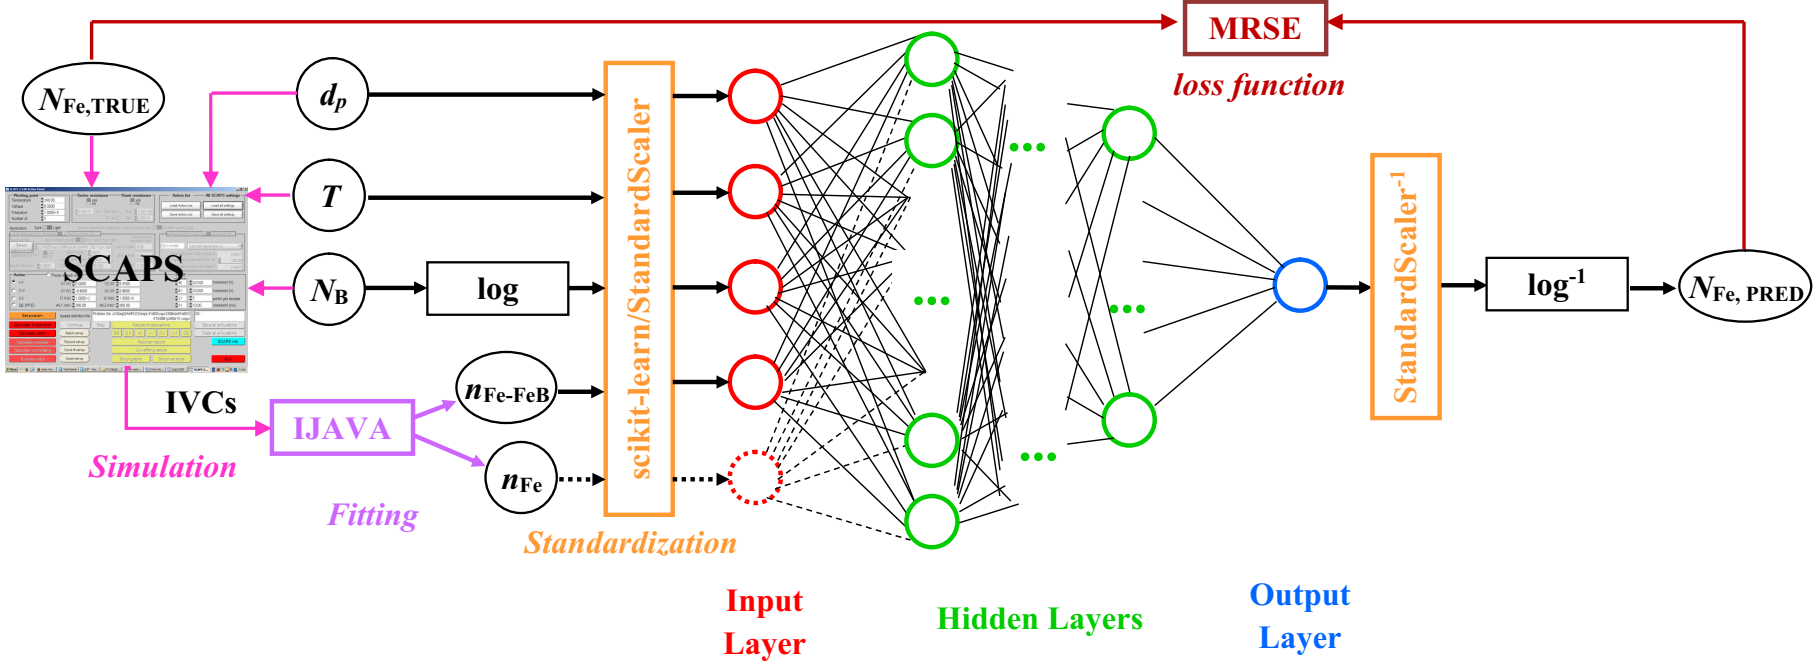
\includegraphics[width=0.8\textwidth]{Chem}
\caption{Schematic of deep learning-based approach  for predicting the iron concentration.
Additional details are discussed in the body of the article.}
\label{fig_chem}
\end{figure}


\section{Simulation Details}

The presented calculation uses $n^+$--$p$--$p^+$ structure:
the emitter layer $n^+$ with the donor concentration $N_D=10^{19}$~cm$^{-3}$ and
the thickness 0.5~$\mu$m;
$p$ and $p^+$ are uniformly doped with boron;
the base $p$ with the thickness $d_p=150$--$240$~$\mu$m is doped with concentration
$N_\mathrm{B}=10^{15}$--$10^{17}$~cm$^{-3}$
and the BSF-layer $p^+$ with the thickness $d_{BSF}$ ($1$~$\mu$m) and the acceptor
concentration $N_{BSF}$ ($5\times10^{18}$~cm$^{-3}$).

The simulations  were carried out over the temperature range $290-340$~K.
The SCAPS setting file was created for each temperature using the following material parameters.
The bandgap $E_G$ and bandgap narrowing $\Delta E_G$ models are, respectively, from P\"{a}ssler \cite{Pasler} and Yan and Cuevas \cite{EgNarrow}:
\begin{eqnarray}
\label{eqEg}
E_G=E_{G0}-\alpha\Theta\left\{\frac{1-3\Delta^2}{e^{\frac{\Theta}{T}}-1}
    +\frac{3\Delta^2}{2}\left(\sqrt[6]{1+\frac{\pi^2}{3(1+\Delta^2)}\left(\frac{2T}{\Theta}\right)^2
    +\frac{3\Delta^2-1}{4}\left(\frac{2T}{\Theta}\right)^3+\frac{8}{3}\left(\frac{2T}{\Theta}\right)^4
    +\left(\frac{2T}{\Theta}\right)^6}-1\right)\right\}\,,\\
\Delta E_G=4.20\times10^{-5}\left[\ln\left(\frac{N_{D}}{10^{14}}\right)\right]^3\,;\qquad
     \Delta E_G=4.72\times10^{-5}\left[\ln\left(\frac{N_{B,BSF}}{10^{14}}\right)\right]^3\,,
\end{eqnarray}
where
$E_{G0}=1.1701$~eV,
$\alpha=3.23\times10^{-4}$~eV/K,
$\Theta=446$~K,
$\Delta=0.51$.
The carrier thermal velocities are calculated from models by Green \citep{Nc:Green}:
\begin{equation}
\label{eqVth}
    \upsilon_{\mathrm{th},n}=\sqrt{\frac{8qkT}{0.28m_0\pi}}\,;\qquad
    \upsilon_{\mathrm{th},p}=\sqrt{\frac{8qkT}{0.41m_0\pi}}\,,
\end{equation}
where
$m_0$ is the free electron mass.
The effective states density masses in the conduction band $m^*_{dC}$ and
the valence band $m^*_{dV}$ are calculated according to models from Couderc et al. \citep{Si_ni_Couderc}:
\begin{eqnarray}
  \left(\frac{m^*_{dC}}{m_0}\right)^{1.5} &=& 1.094-1.312\times10^{-5}T+6.753\times10^{-7}T^2+4.609\times10^{-10}T^3\,, \\
  \left(\frac{m^*_{dV}}{m_0}\right)^{1.5} &=& 0.3426+3.376\times10^{-3}T-4.689\times10^{-6}T^2+2.525\times10^{-9}T^3\,.
\end{eqnarray}
The carrier mobilities and the free carrier effective masses  were taken from Klaassen \cite{KLAASSEN953}
and O'Mara et al. \cite{OMara}, respectively.
The temperature and doping dependencies of Auger recombination coefficients are calculated from models by Altermatt et al. \cite{Si_Auger}:
\begin{eqnarray}
% \nonumber to remove numbering (before each equation)
   \nonumber C_{p} (T)&=& (7.91\times10^{-32}-4.13\times10^{-35}T+3.59\times10^{-37}T^2)\\
  &&\times\left(1+\left(564812T^{-1.6545}-1\right)\left(1-\tanh\left[\left\{\frac{p}{5\times10^{16}}\right\}^{0.29}\right]\right)\right)\,, \\
   C_{n} (T)&=& 2.8\times10^{-31}
  \times\left(1+\left(235548T^{-1.5013}-1\right)\left(1-\tanh\left[\left\{\frac{n}{5\times10^{16}}\right\}^{0.34}\right]\right)\right)\,.
\end{eqnarray}
The band-to-band radiation recombination coefficient was taken from Nguyen et al. \cite{Si_BtB}.

The outside surface recombination with electron and hole velocities $10^3$~cm/s was taken into account.

The simulations are carried out under the assumption that the defect–assisted recombination corresponds to the
iron–related deep levels only.
As the base and the SBF-layer uniform contaminant, iron is assumed to be in concentration
$N_{\mathrm{Fe}}=10^{10}$--$10^{13}$~cm$^{-3}$.
The simulations have been performed for the following two cases.
In the first one, the concentration of total dissolved iron is given by a sum of
concentrations of the interstitial iron $\mathrm{Fe}_i$
and the trigonal iron-boron pair $\mathrm{Fe}_i\mathrm{B}_s$:
\begin{equation}\label{eqNFeB}
  N_{\mathrm{Fe}}=N_{\mathrm{Fe}_i}+N_{\mathrm{Fe}_i\mathrm{B}_s}\,.
\end{equation}
The defect distributions are inhomogeneous, and depend on the Fermi level $F$ position, and are given by
\cite{MurphyJAP2011,FeB:kinetic}:
\begin{equation}
\label{eqNFeB}
    \frac{N_{\mathrm{FeB}}}{N_{\mathrm{Fe}}}=\frac{N_\mathrm{B}10^{-23}\exp\left(-\frac{E_b}{kT}\right)}
     {\left[1+\frac{N_\mathrm{B}}{10^{23}}\exp\left(-\frac{E_b}{kT}\right)\right]\left[1+\exp\left(-\frac{F-E_{\mathrm{Fe}_i}}{kT}\right)\right]}\,,
     \quad N_{\mathrm{Fe}_i}=N_{\mathrm{Fe}}-N_{\mathrm{FeB}}\,,
\end{equation}
where
$E_b=0.582$~eV is the binding energy of the $\mathrm{Fe}_i\mathrm{B}_s$ pairs,
$E_{\mathrm{Fe}_i}$ is the donor level, associated with $\mathrm{Fe}_i$.
This case corresponds to the equilibrium condition and in this article will be referred to as ``Fe-FeB''.

In the second one, the $\mathrm{Fe}_i$ is suggested to be presented only with homogeneous distribution ($N_{\mathrm{Fe}_i}=N_{\mathrm{Fe}}$).
This case can be realized by heat treatment (210$^\circ$C, 3~min) \cite{FeB_Zong} or intense illumination \cite{FeBLight2} and will be referred as ``Fe'' hereafter.

The donor level $E_{\mathrm{Fe}_i} = E_V+0.394$~eV
with electron $\sigma_{n,{\mathrm{Fe}}}=3.47\times10^{-11}T^{-1.48}$~cm$^2$ and
hole $\sigma_{p,{\mathrm{Fe}}}=4.54\times10^{-16}\exp\left(-\frac{0.05}{kT}\right)$~cm$^2$ capture cross-sections \cite{MurphyJAP2011,ROUGIEUX2018}
is associated with $\mathrm{Fe}_i$ in simulations.
The donor level $E_{\mathrm{FeB}}^\mathrm{D}= E_V+0.10$~eV,
$\sigma_{n,{\mathrm{FeB}}}^\mathrm{D}=4\times10^{-13}$~cm$^2$,
$\sigma_{p,{\mathrm{FeB}}}^\mathrm{D}=2\times10^{-14}$~cm$^2$
and acceptor level $E_{\mathrm{FeB}}^\mathrm{A}= E_C-0.26$~eV,
$\sigma_{n,{\mathrm{FeB}}}^\mathrm{A}=5.1\times10^{-9}T^{-2.5}$~cm$^2$,
$\sigma_{p,{\mathrm{FeB}}}^\mathrm{A}=3.32\times10^{-10}\exp\left(-\frac{0.262}{kT}\right)$~cm$^2$
\cite{Istratov1999,MurphyJAP2011,ROUGIEUX2018}
are used for $\mathrm{Fe}_i\mathrm{B}_s$.

The dark forward IV characteristics were generated by SCAPS over a voltage range up to $0.45$~V.
According to the two-diode model, the dark SC current is given by \citep{Breitenstein2013}
\begin{equation}
\label{eqIVd}
    I=I_{01}\left[\exp\left(-\frac{q(V-R_sI)}{kT}\right)-1\right]
      + I_{02}\left[\exp\left(-\frac{q(V-R_sI)}{nkT}\right)-1\right]
      +\frac{V-R_sI}{R_{sh}}\,,
\end{equation}
where
$I_{01}$ and $I_{02}$ are the saturation currents,
$R_{sh}$ and $R_s$ are the shunt and series resistances.
The two-diode model is often applied for description of real Si SCs
and we used Eq.~\ref{eqIVd} to fit the simulated data by taking $n$, $I_{01}$, $I_{02}$,
$R_{sh}$, and $R_s$ as fitting parameters.
The fitting was performed by using the meta--heuristic method IJAVA \cite{IJAVA}.
It should be noted that influence of both $R_s$ (obtained values $<10^{-2}$~$\Omega$) and $R_{sh}$
(obtained values $>10^{18}$~$\Omega$) can be neglected in simulated IV.

It is the ideality factor value $n$ which is used in our further calculation.
The ideality factors, which are obtained in  Fe-case and Fe-FeB-case,
are referred to as  $n_\mathrm{Fe}$ and $n_\mathrm{Fe-FeB}$ hereafter.
The typical simulated dependencies of  the ideality factor are shown in Fig.~\ref{fig_nValues}.
The detailed discussion about $n_\mathrm{Fe}$ and $n_\mathrm{Fe-FeB}$  values are presented elsewhere \cite{OlikhJPS},
however it should be noted that
(i)~$n$ can take equal values for different  values of SC parameters;
(ii)~dependencies of $n_\mathrm{Fe}$ and $n_\mathrm{Fe-FeB}$ vary not only in absolute values but although in behavior slightly.

\begin{figure}[t]
\centering
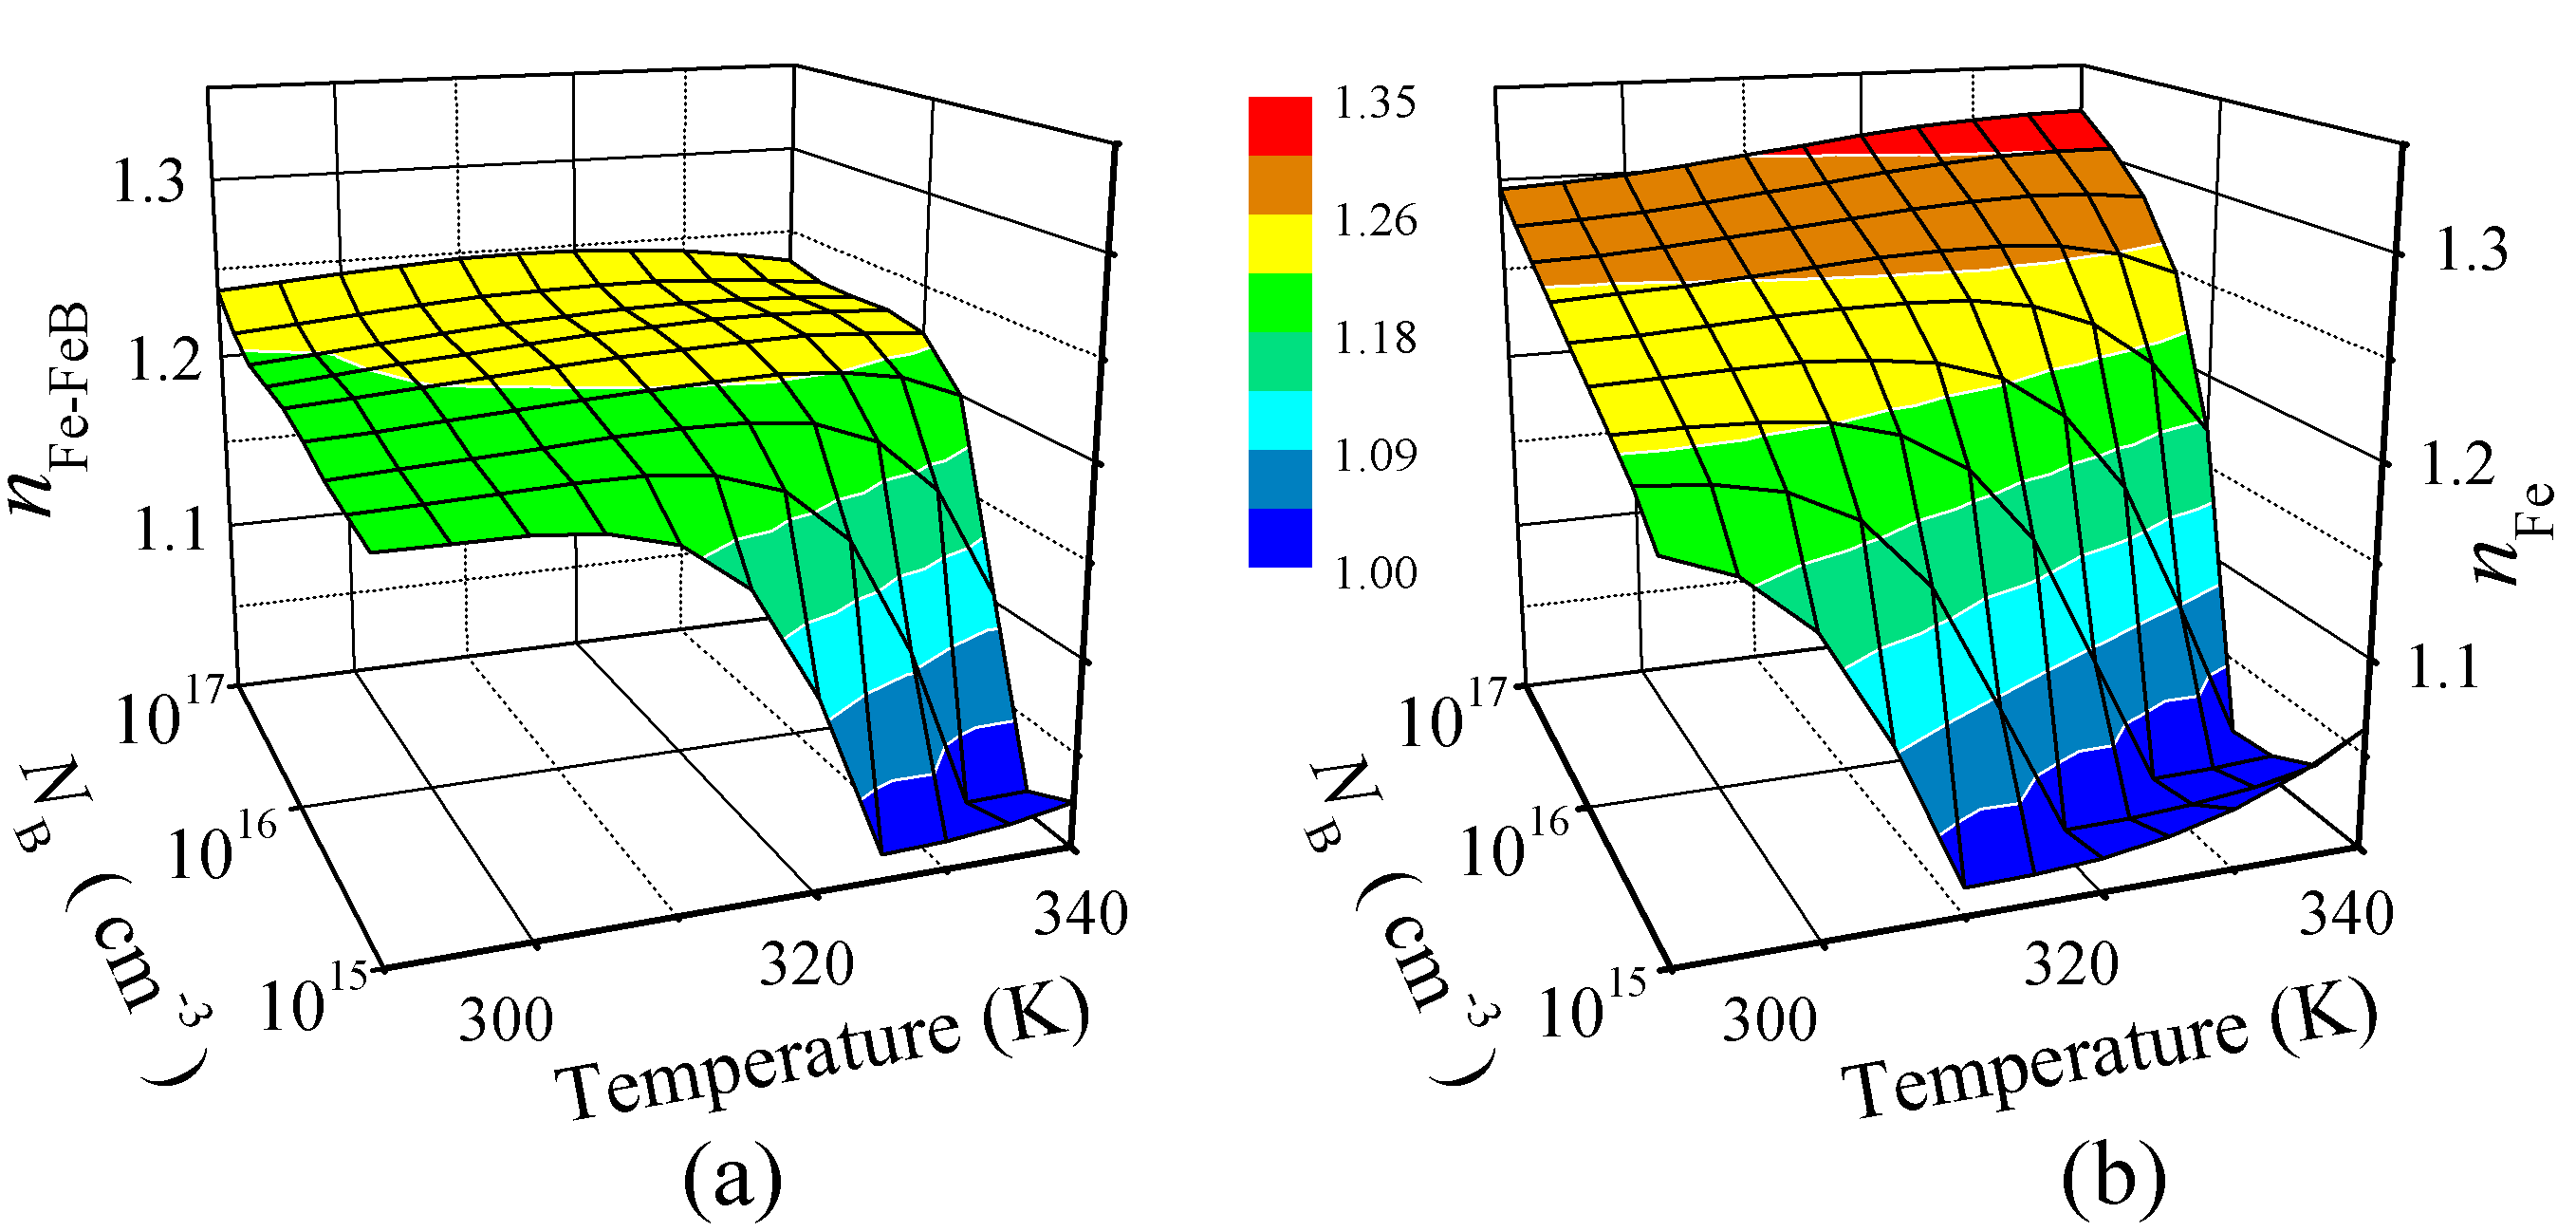
\includegraphics[width=0.48\textwidth]{Fig1a}
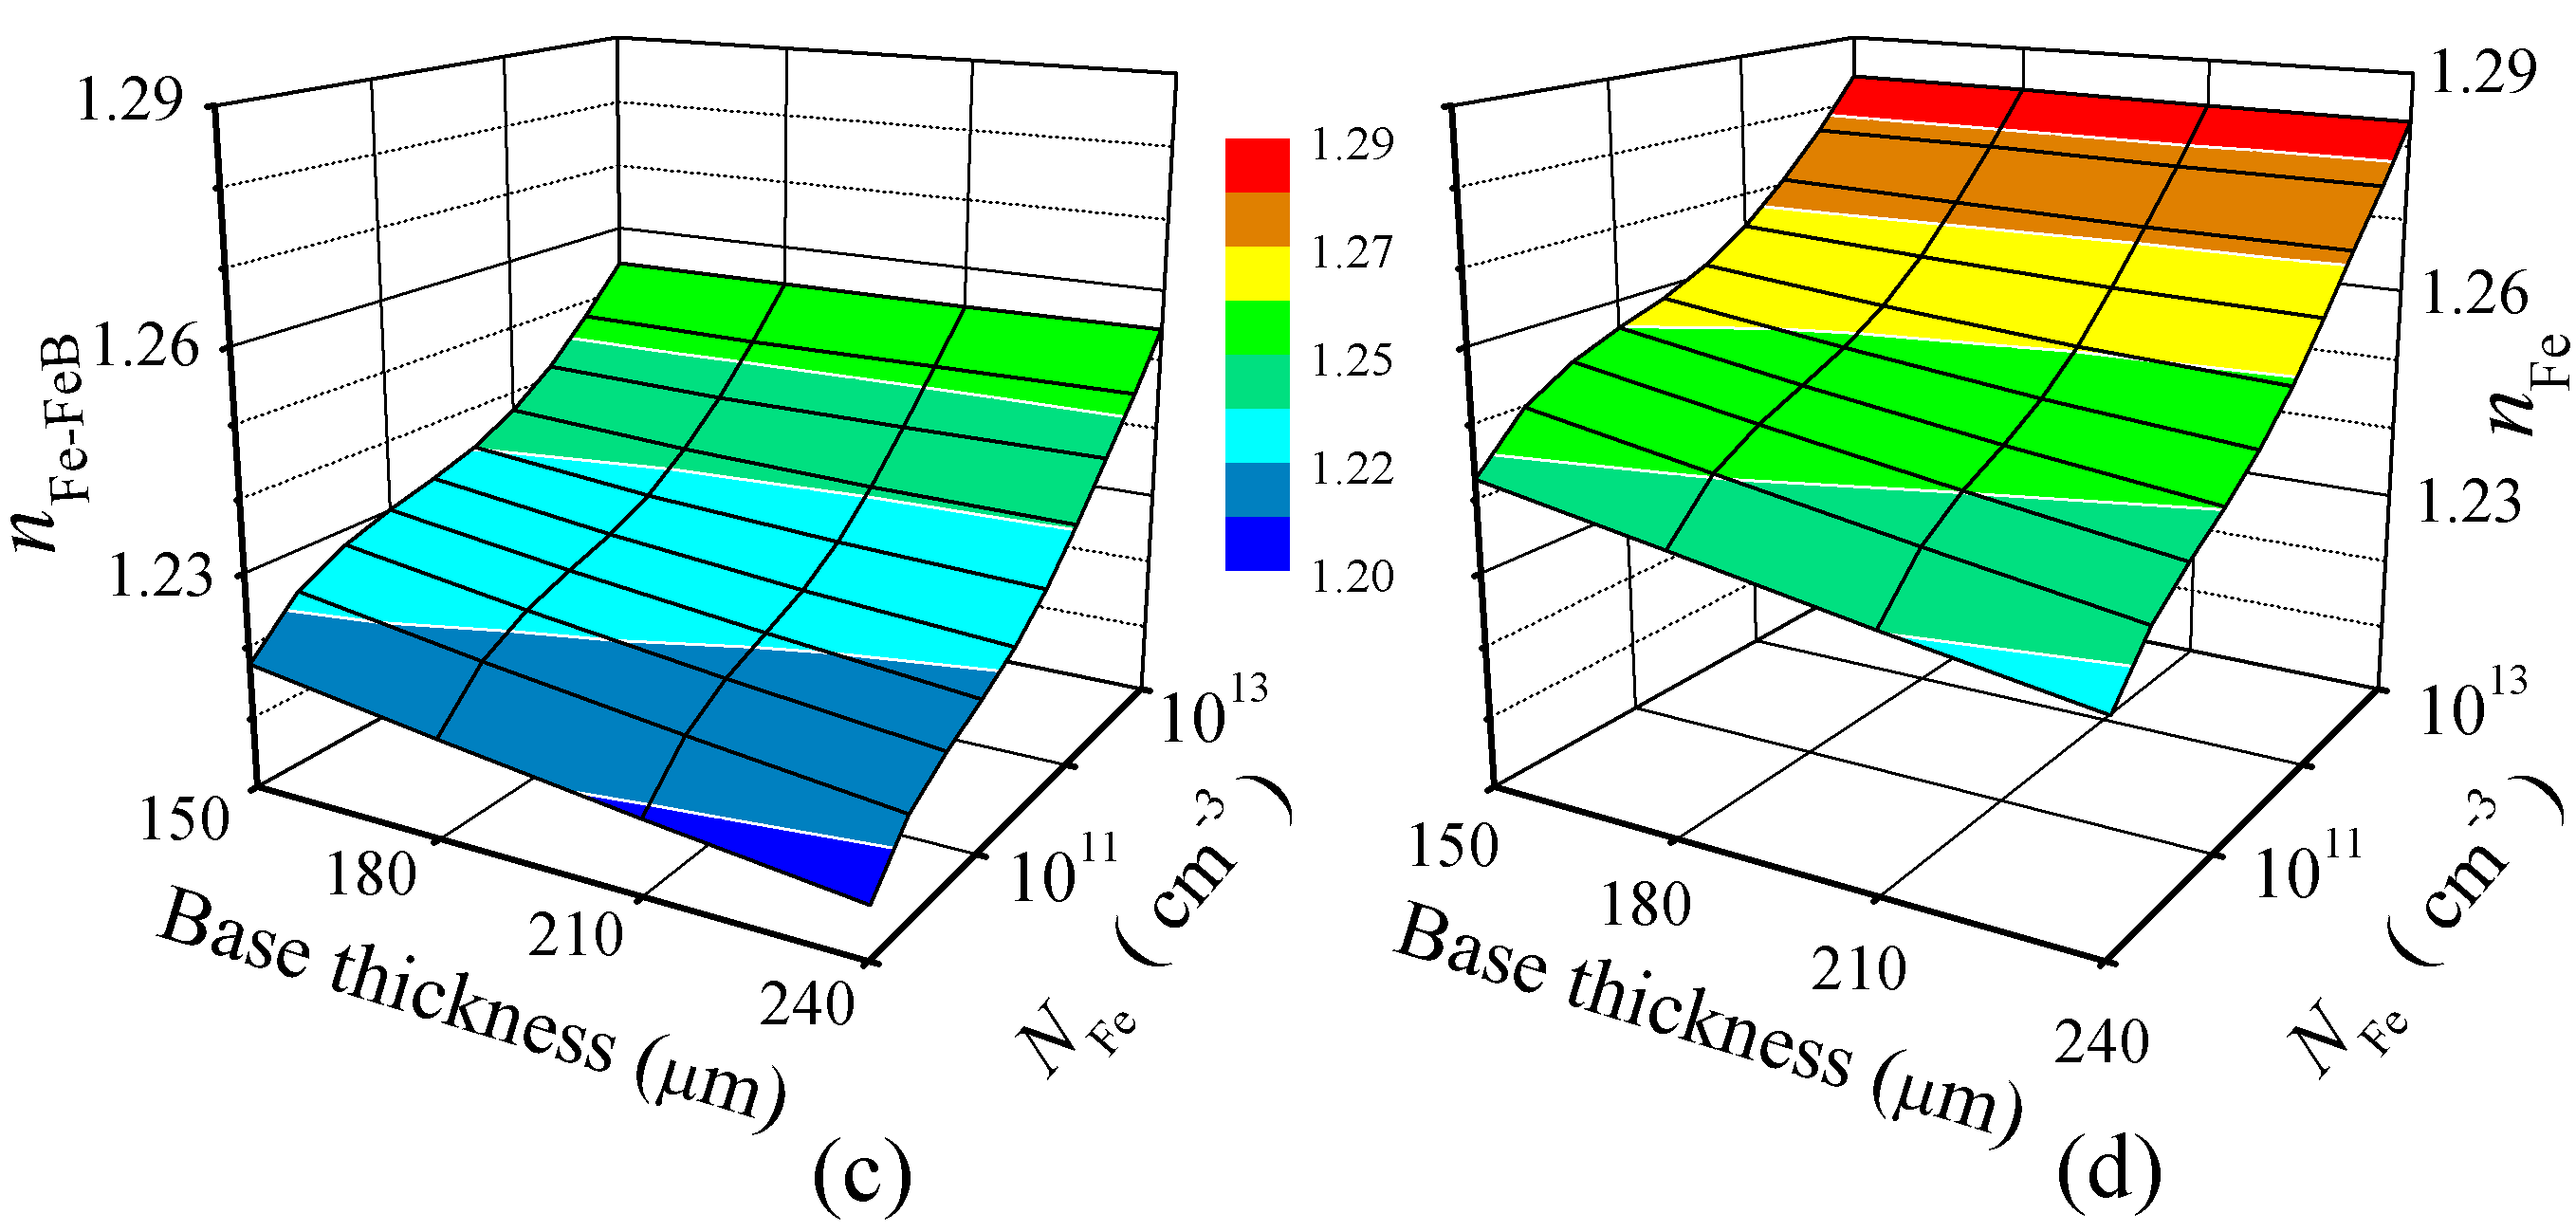
\includegraphics[width=0.48\textwidth]{Fig1b}
\caption{Ideality factor versus temperature and boron concentration (a, b)
or base thickness and iron concentration (c,d).
The Fe-FeB-case (a, c) and Fe-case (b, d).
$N_\mathrm{Fe}=10^{10}$~cm$^{-3}$ (a,b),
$d_p=180$~$\mu$m (a, b),
$N_\mathrm{B}=10^{16}$~cm$^{-3}$ (c, d),
$T=320$~K (c, d).
}
\label{fig_nValues}
\end{figure}

\section{Deep neural network models}

Training a deep neural network requires a large number of samples.
In order to build a training dataset, we used IV characteristics, which
are simulated with using of 4 $d_p$ values, 9 $N_\mathrm{B}$ values, 11 $T$ values and 19 $N_{\mathrm{Fe}}$ values.
These base thickness, doping level, temperature, and iron concentration values are regularly (for $T$ and $d_p$ in linear scale, for $N_{\mathrm{Fe}}$ and $N_\mathrm{B}$ in logarithmic scale) distributed over the  ranges $150$--$240$~$\mu$m, $10^{15}$--$10^{17}$~cm$^{-3}$, $290-340$~K, and
$10^{10}$--$10^{13}$~cm$^{-3}$, respectively.
Thus, 7524 IV characteristics are simulated in Fe-case as well as in Fe-FeB-case to build a training dataset.

Besides, several test datasets are prepared.
The $d_p$, $N_\mathrm{B}$, and $N_{\mathrm{Fe}}$ values, which equal to  values from training dataset, and $T$ values, which is divergent from training dataset, are used to build the test dataset, labeled ``T-varied''.
This dataset is based on 894 pairs of IV characteristics.
The similar approach was used to prepare ``d-varied'' (1189 samples), ``Fe-varied'' (856 samples), and ``B-varied'' (514 samples) test datasets.
The base thickness, doping level, temperature, and iron concentration values, which are divergent from training dataset values, are used to prepare ``All-varied'' (684 samples).

The precise values of parameters are listed in Supplementary Material.

We have tried to construct the DNN, which can estimate iron contamination by using
SC parameters ($d_p$ and $N_\mathrm{B}$),  measurement temperature, and the result of IV fitting (ideality factor value).
As it is shown in Fig.~\ref{fig_chem} two DNNs with different input parameters were under consideration.
The input sample of the first one consist of $\{d_p,\log N_\mathrm{B},T,n_\mathrm{Fe-FeB}\}$.
In practice, this input set can be obtained from one dark IV measurement.
This neural network is referred to as DNN$_\mathrm{FeFeB}$ hereafter.
The second one uses  $\{d_p,\log N_\mathrm{B},T,n_\mathrm{Fe-FeB},n_\mathrm{Fe}\}$ in input layer.
In practice, the obtaining of such a set requires additional SC processing (e.g., intense illumination) and two IV measurements.
The label  DNN$_\mathrm{FeFeB-Fe}$ is used below.

The dense deep neural network was implemented through the high-level Keras API provided by TensorFlow \cite{Keras}.
The input layers consist of 4 or 5 nodes --- see Fig.~\ref{fig_chem}.
1 node and linear activation were used in the output layer.
The five configurations oh hidden layers were under consideration:
(i)~``pipe'': each hidden layer contains equal number of nodes;
(ii)~``trapezium'': six hidden layers, number of neurons linearly decreases from 100\% (first layer) to 50\% (last layer);
(iii)~``triangle'': ten layers, number of neurons linearly decreases from 100\% (first layer) to 10\% (last layer);
(iv)~``butterfly'': two serial reflected trapezium configurations;
(v)~``fir'': two serial trapezium configurations.

The mean squared relative error (MSRE) was chosen as the loss function:
\begin{equation}
\label{eqMSRE}
    \mathrm{MSRE}=\frac{1}{N_s}\sum_{i=1}^{N_s}\frac{(N_\mathrm{Fe,TRUE,i}-N_\mathrm{Fe,PRED,i})^2}{N_\mathrm{Fe,TRUE,i}\cdot N_\mathrm{Fe,PRED,i}}\,,
\end{equation}
where
$N_s$ is the number of samples in dataset,
$N_\mathrm{Fe,TRUE,i}$ is the iron concentration, which was used in simulation of $i$--th sample,
$N_\mathrm{Fe,PRED,i}$ is the DNN prediction for $i$--th sample.

Hyperparameters include the number of nodes for the first hidden layer,
the number of hidden layers (in pipe configuration),
the batch size,
the activation function,
the optimizer,
the learning rate,
the preprocessing method,
the dropout rate,
the regularization function,
the regularization rate,
and the weight initializer.
A grid search (coarse tuning to limit one hyperparameter) and random search (fine tuning) were performed over the predefined hyperparameter space, shown in Table~\ref{tabHP}, and the best hyperparameter combination is chosen.


\begin{table}%[width=\linewidth,cols=2,pos=h]
\caption{Hyperparameter space for DNNs.}\label{tabHP}
\begin{tabular}{ll}%{\tblwidth}{@{} LL@{} }
\headrow
\thead{Hyperparameter}& \thead{Values}\\
%Hyperparameter & Values\\
%\midrule
\# nodes for first
hidden layer & 30, 40, 50, 75, 100, 120, 150 \\
\# hidden layers & 4, 5, 6, 8, 10, 15 \\
 batch size & 8, 16, 32, 64, 128 \\
activation function & ReLu, sigmoid, tanh, SELU, ELU \\
optimizer & SGD, RMSprop, Adam, Adadelta, Adagrad, Adamax, Nadam, Ftrl \\
learning rate & $10^{-5}$, $10^{-4}$, $10^{-3}$, $10^{-2}$\\
\# epochs & 100, 300, 400, 600, 1000, 1500\\
preprocessing method & StandartScaler, MinMaxScaler \\
regularization function& None, L2, L1, Dropout\\
regularization rate & $10^{-5}$, $10^{-4}$, $10^{-3}$, $10^{-2}$\\
dropout rate & 0.2, 0.3, 0.4, 0.5 \\
weight initializer& Xavier Normal or Uniform, He Normal or Uniform, Random Normal or Uniform, Ones\\
\hline
\end{tabular}
\end{table}

10--fold cross--validation was used to estimate DNN training.
The MSRE, coefficient of determination $R^2$, and coefficient of correlation $R$ were
three metrics used to evaluate the performance of the DNN models on test datasets.
Finally, to increase a DNNs performance, the full dataset, which consists of training dataset and all test datasets,  was used for the training models.

\section{Results and Discussion}
\subsection{Synthetic IV curves}

The results of the hyperparameter search are listed in Table~\ref{tabChosenHP}.
In particular, the trapezium and pipe configurations are chosen for DNN$_\mathrm{FeFeB}$ and DNN$_\mathrm{FeFeB-Fe}$ respectively.


\begin{table}%[width=.9\linewidth,cols=3,pos=h]
\caption{Chosen hyperparameter combinations.}\label{tabChosenHP}
\begin{tabular}{lll}%{\tblwidth}{@{} LLL@{} }
\headrow
\thead{Hyperparameter} & \thead{DNN$_\mathrm{FeFeB}$}&\thead{DNN$_\mathrm{FeFeB-Fe}$}\\
\# nodes for hidden layers & 120, 108, 96, 84, 72, 60& 100, 100, 100, 100 \\
 batch size & 32 &32 \\
activation function & ReLu & ELU \\
optimizer & Adamax & Adamax\\
learning rate & $10^{-3}$& $10^{-3}$\\
\# epochs & 400 & 1500\\
preprocessing method & StandartScaler& StandartScaler\\
regularization function& None& None\\
weight initializer& Xavier Normal & Xavier Normal\\
\hline
\end{tabular}
\end{table}

The training and test results of DNN$_\mathrm{FeFeB}$ are presented in Table~\ref{table_CV},
Table~\ref{table_MSRE}, and Fig.~\ref{fig_TrDNN1}.
As we can see, that MSRE of DNN$_\mathrm{FeFeB}$ prediction is sufficiently large.
But it should be noted, that the fraction of prediction with a big difference
between  $N_\mathrm{Fe,TRUE,i}$ and $N_\mathrm{Fe,PRED,i}$ is not numerous in most cases.
Thus squared relative error (SRE) does not exceed 0.05 for 87\%, 88\%, and 96\% samples from
T-varied, d-varied and Fe-varid datasets respectively --- see bars in Fig.~\ref{fig_TrDNN1}.
For the B-varied dataset (with doping level value, non--used in the training dataset)
the biggest $\mathrm{MSRE}=1.06$  connects to the occurrence of some samples with  a really big SRE (>20).
While  SRE is less than 0.05 in 54\% of samples from the B-varied test dataset.
The worst predictions are quite expectedly to be observed for the All-varied dataset:
$R^2$ equals 0.813 and SRE is less than 0.05 for 18\% only.
On the other hand, the Fe-varied dataset is most similar to real demand.
And determination and correlation coefficients are high enough (0.991 and 0.996) in this case.

\begin{table}%[width=.9\linewidth,cols=3,pos=h]
\caption{Results of 10--fold cross--validation}\label{table_CV}
\begin{tabular}{lcc}%{\tblwidth}{@{} LLL@{} }
\headrow
\thead{Dataset} & \multicolumn{2}{c}{MSRE}\\
\headrow
 & \thead{DNN$_\mathrm{FeFeB}$}&\thead{DNN$_\mathrm{FeFeB-Fe}$}\\
training&$0.31\pm0.07$&$0.03\pm0.01$ \\
full&$0.28\pm0.05$& $0.03\pm0.01$\\
\hline
\end{tabular}
\end{table}


\begin{table}%[width=.9\linewidth,cols=7,pos=h]
\caption{DNN's testing results}\label{table_MSRE}
\begin{tabular}{lcccccc}%{\tblwidth}{@{} LLLLLLL@{} }
\headrow
\thead{Dataset} & \multicolumn{3}{c}{DNN$_\mathrm{FeFeB}$}& \multicolumn{3}{c}{DNN$_\mathrm{FeFeB-Fe}$}\\
\headrow
 & \thead{MSRE} & \thead{$R^2$}& \thead{$R$} & \thead{MSRE} & \thead{$R^2$}& \thead{$R$}\\
T--varied&0.41 &0.936 &0.967 & 0.020& 0.994&0.997 \\
d--varied&0.37 &0.961&0.980& 0.018&0.996&0.998\\
B--varied&1.06&0.881&0.939& 0.084&0.991&0.995\\
Fe--varied&0.06 &0.991&0.996& 0.005&0.999&0.999\\
All--varied&0.54 &0.813&0.901& 0.138&0.948&0.974\\
\hline
\end{tabular}
\end{table}

\begin{figure}[tb]
\centering
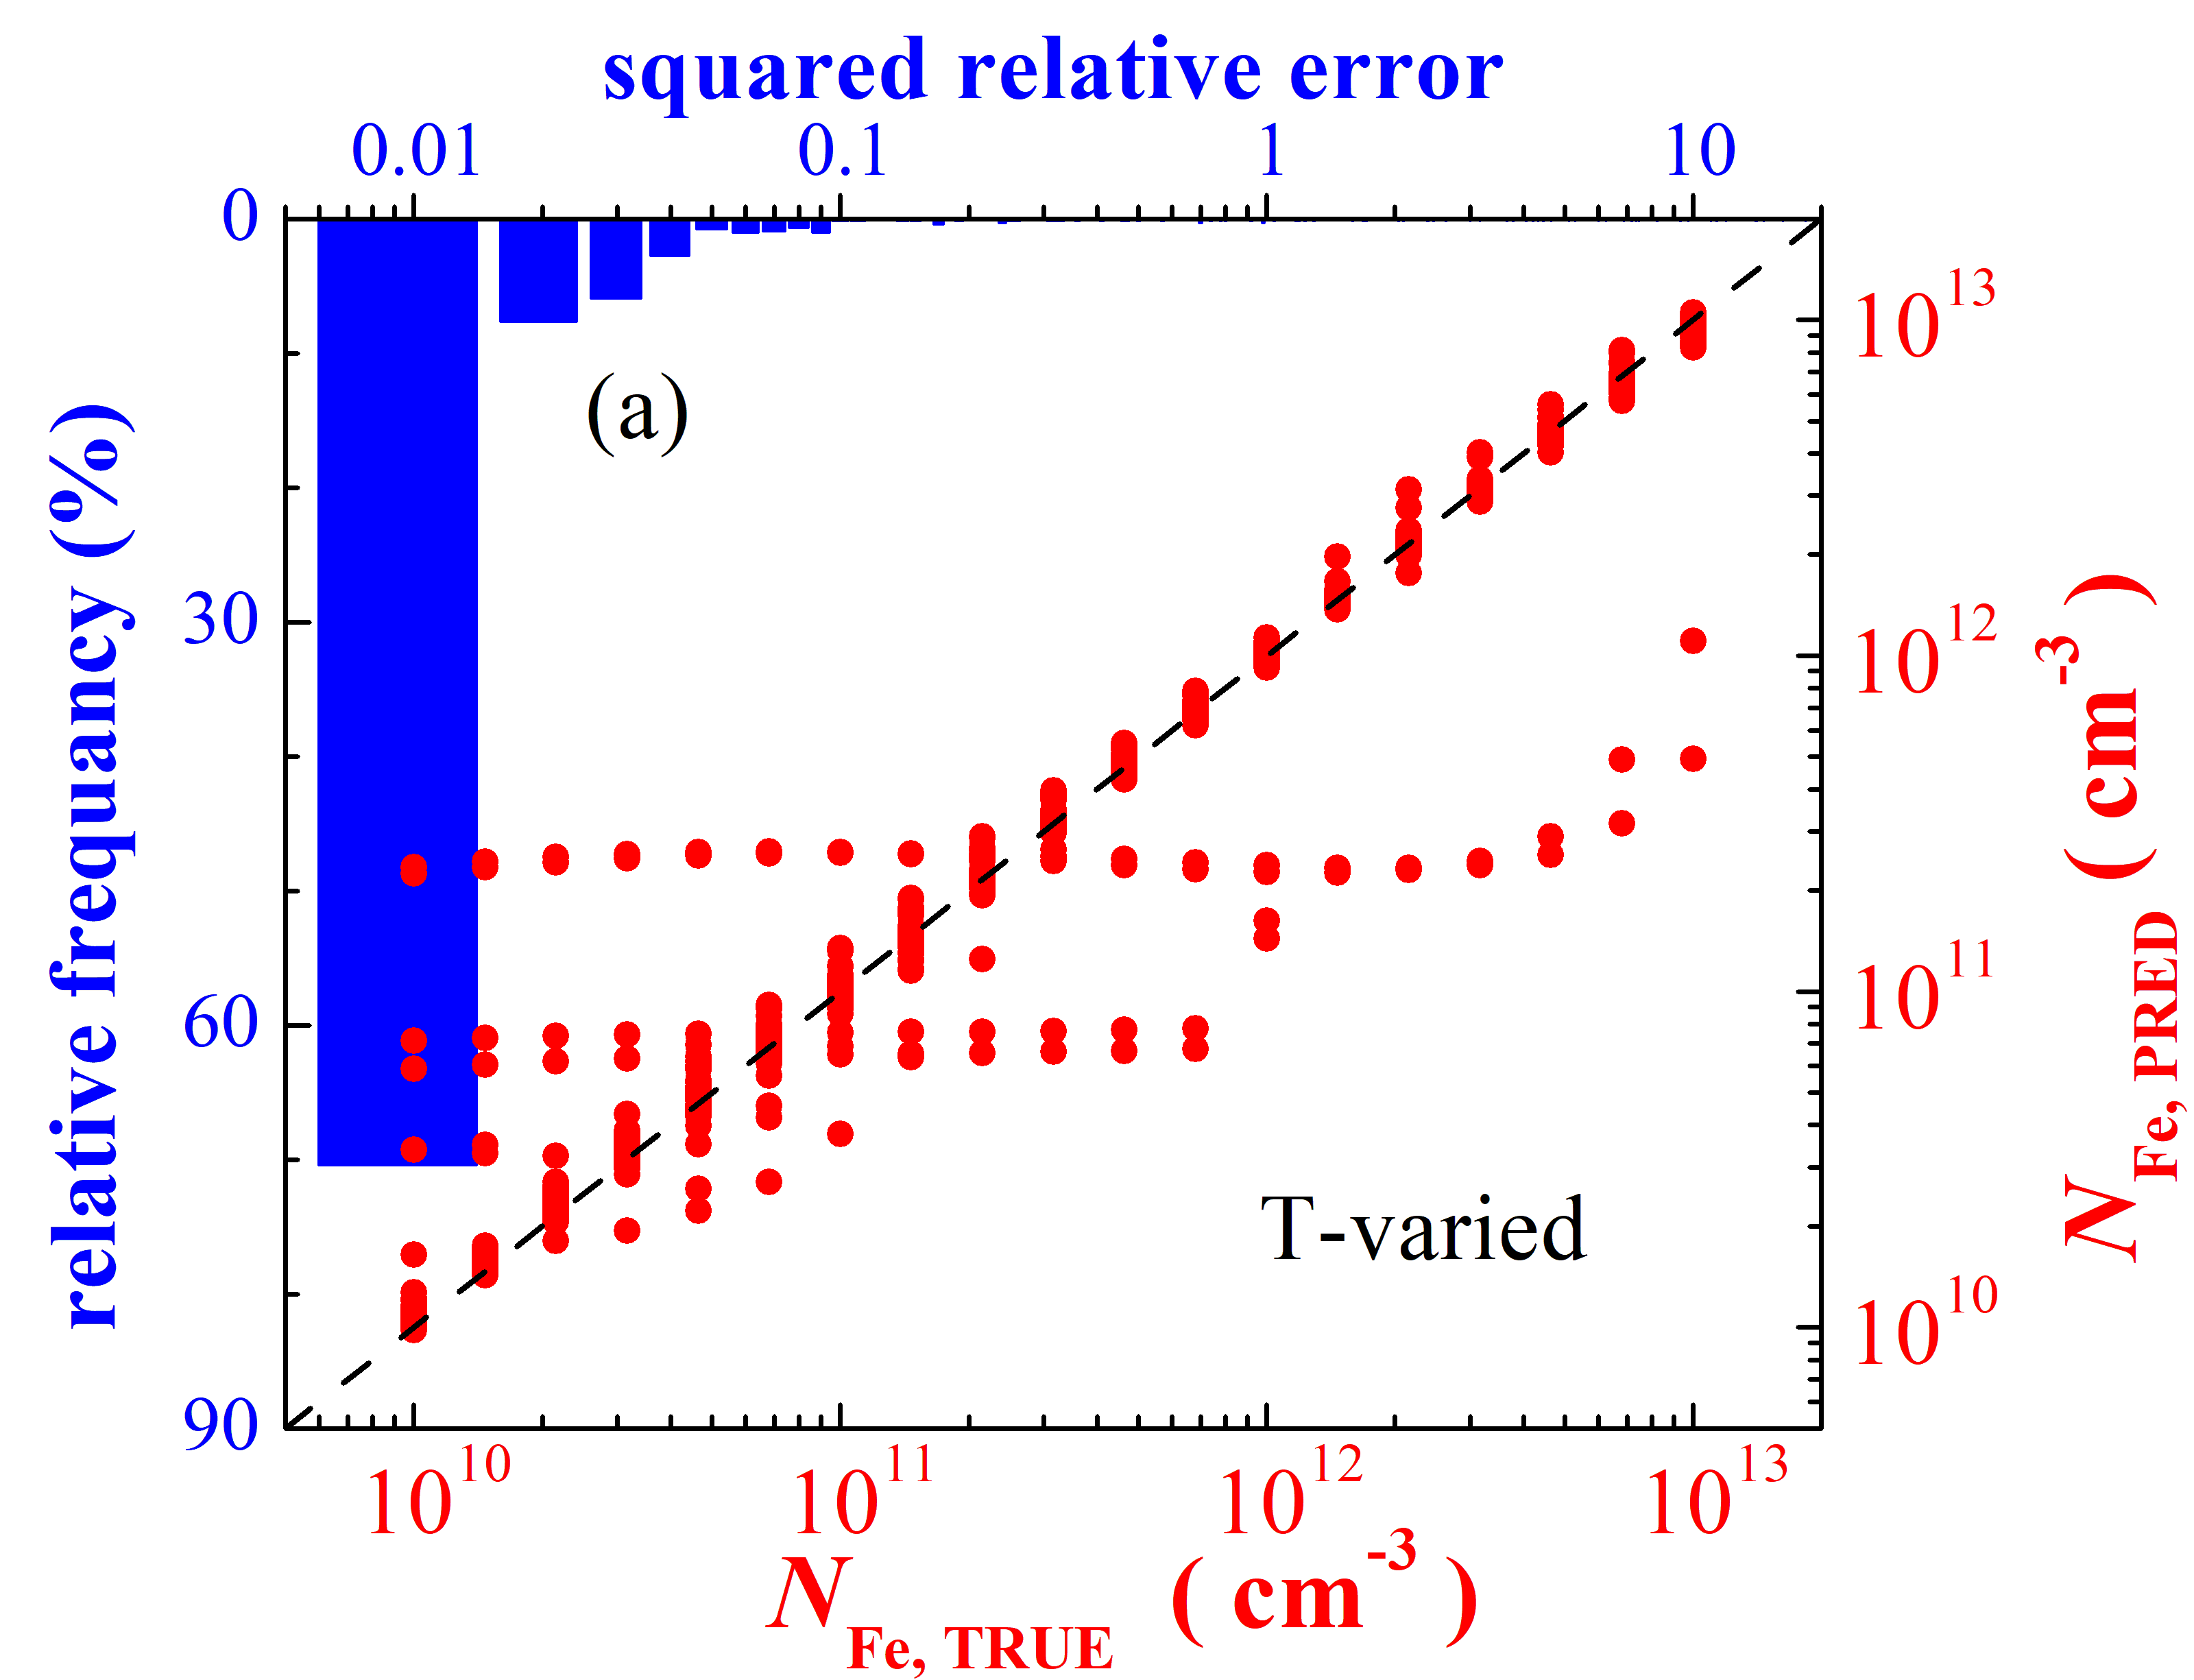
\includegraphics[width=0.32\textwidth]{F3a}
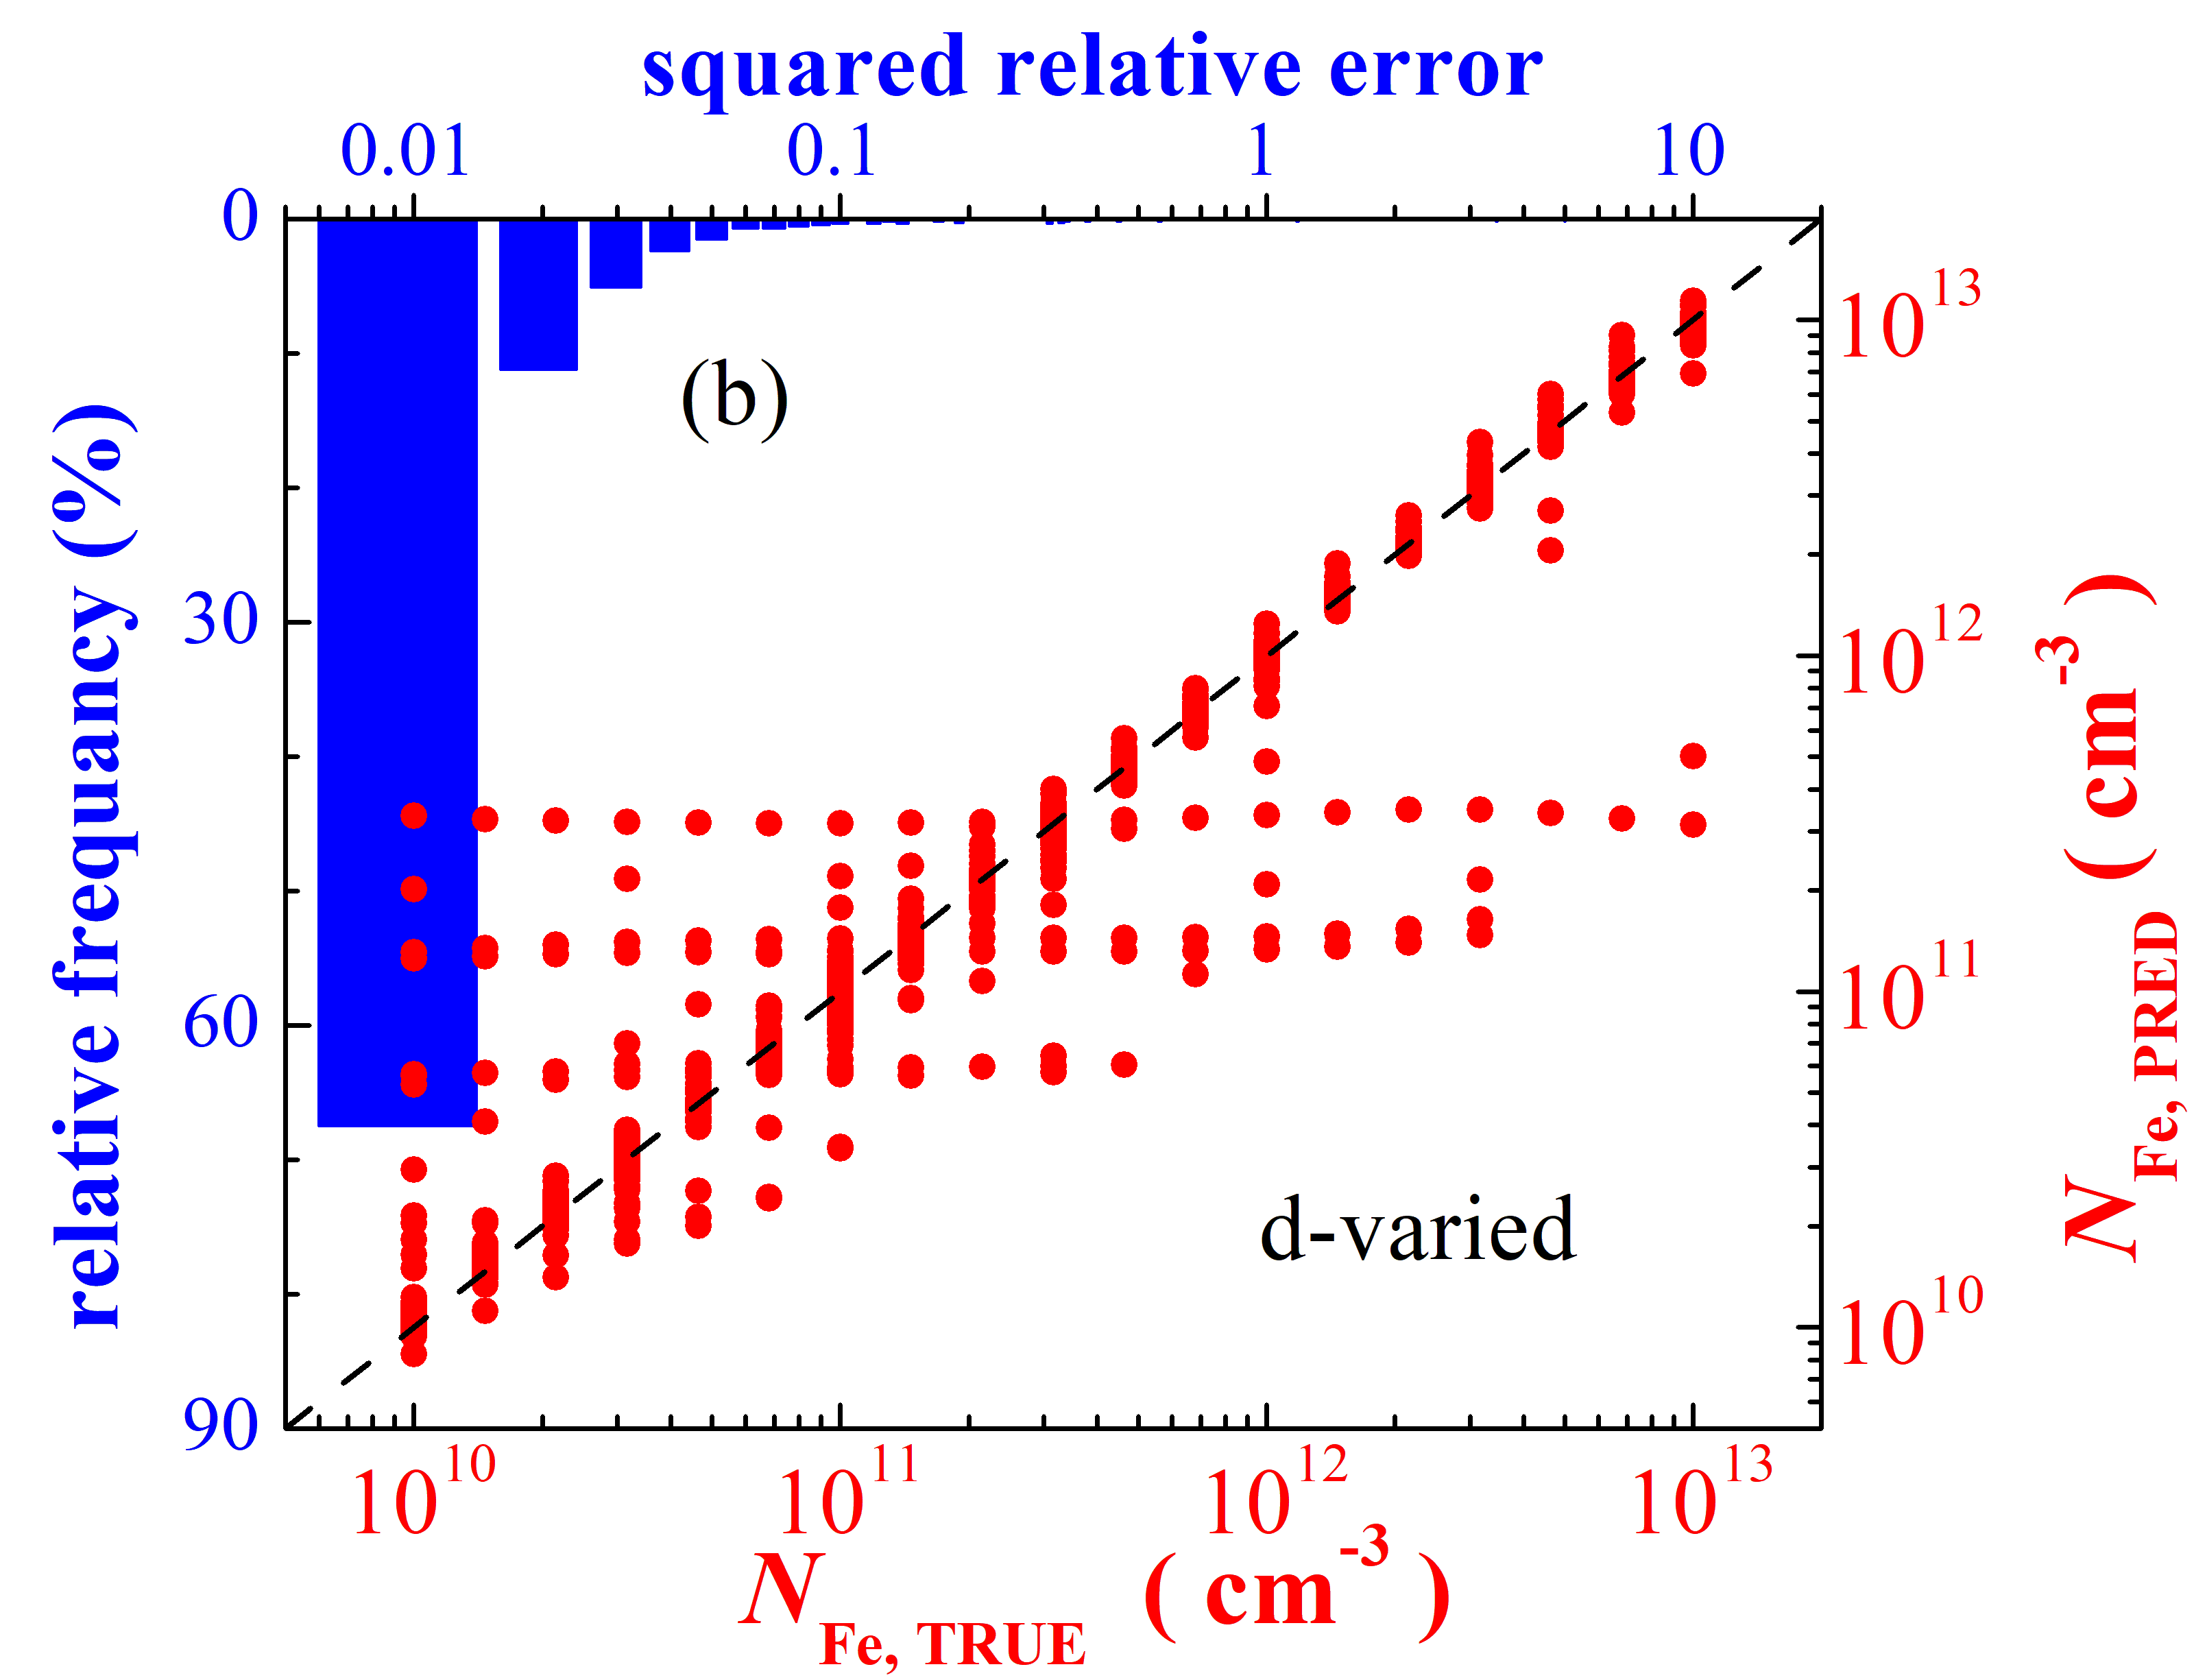
\includegraphics[width=0.32\textwidth]{F3b}
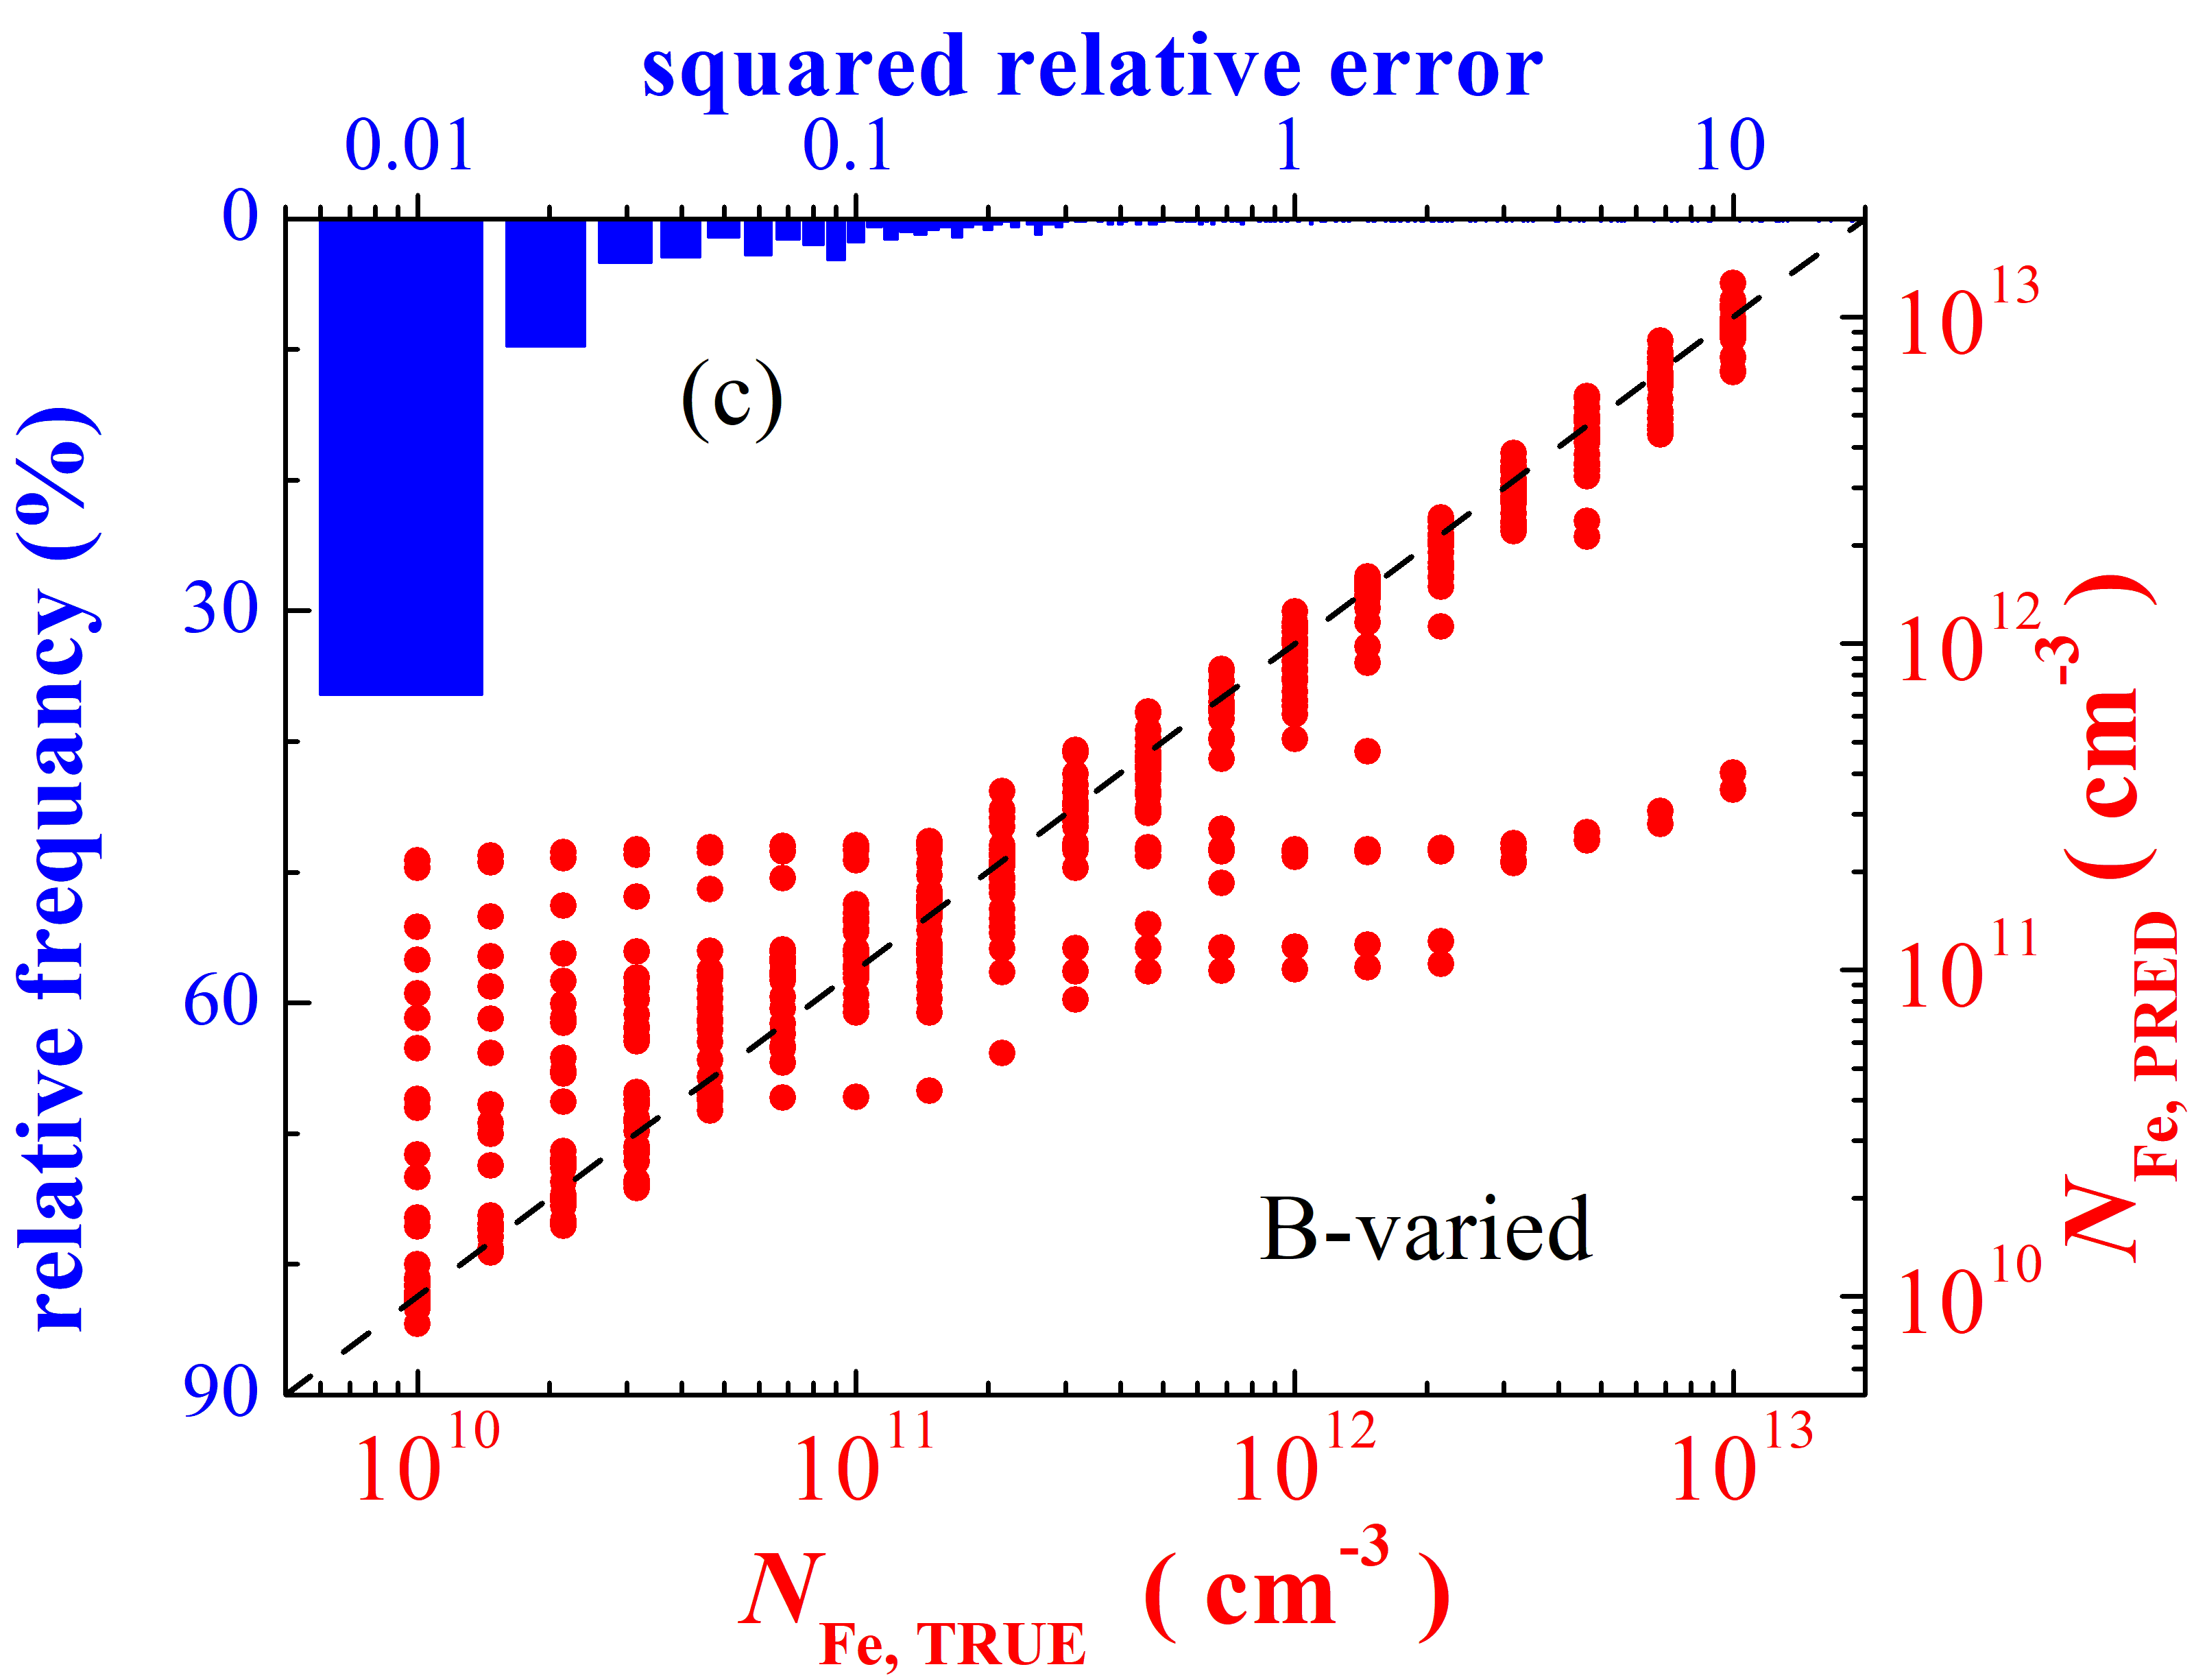
\includegraphics[width=0.32\textwidth]{F3c}
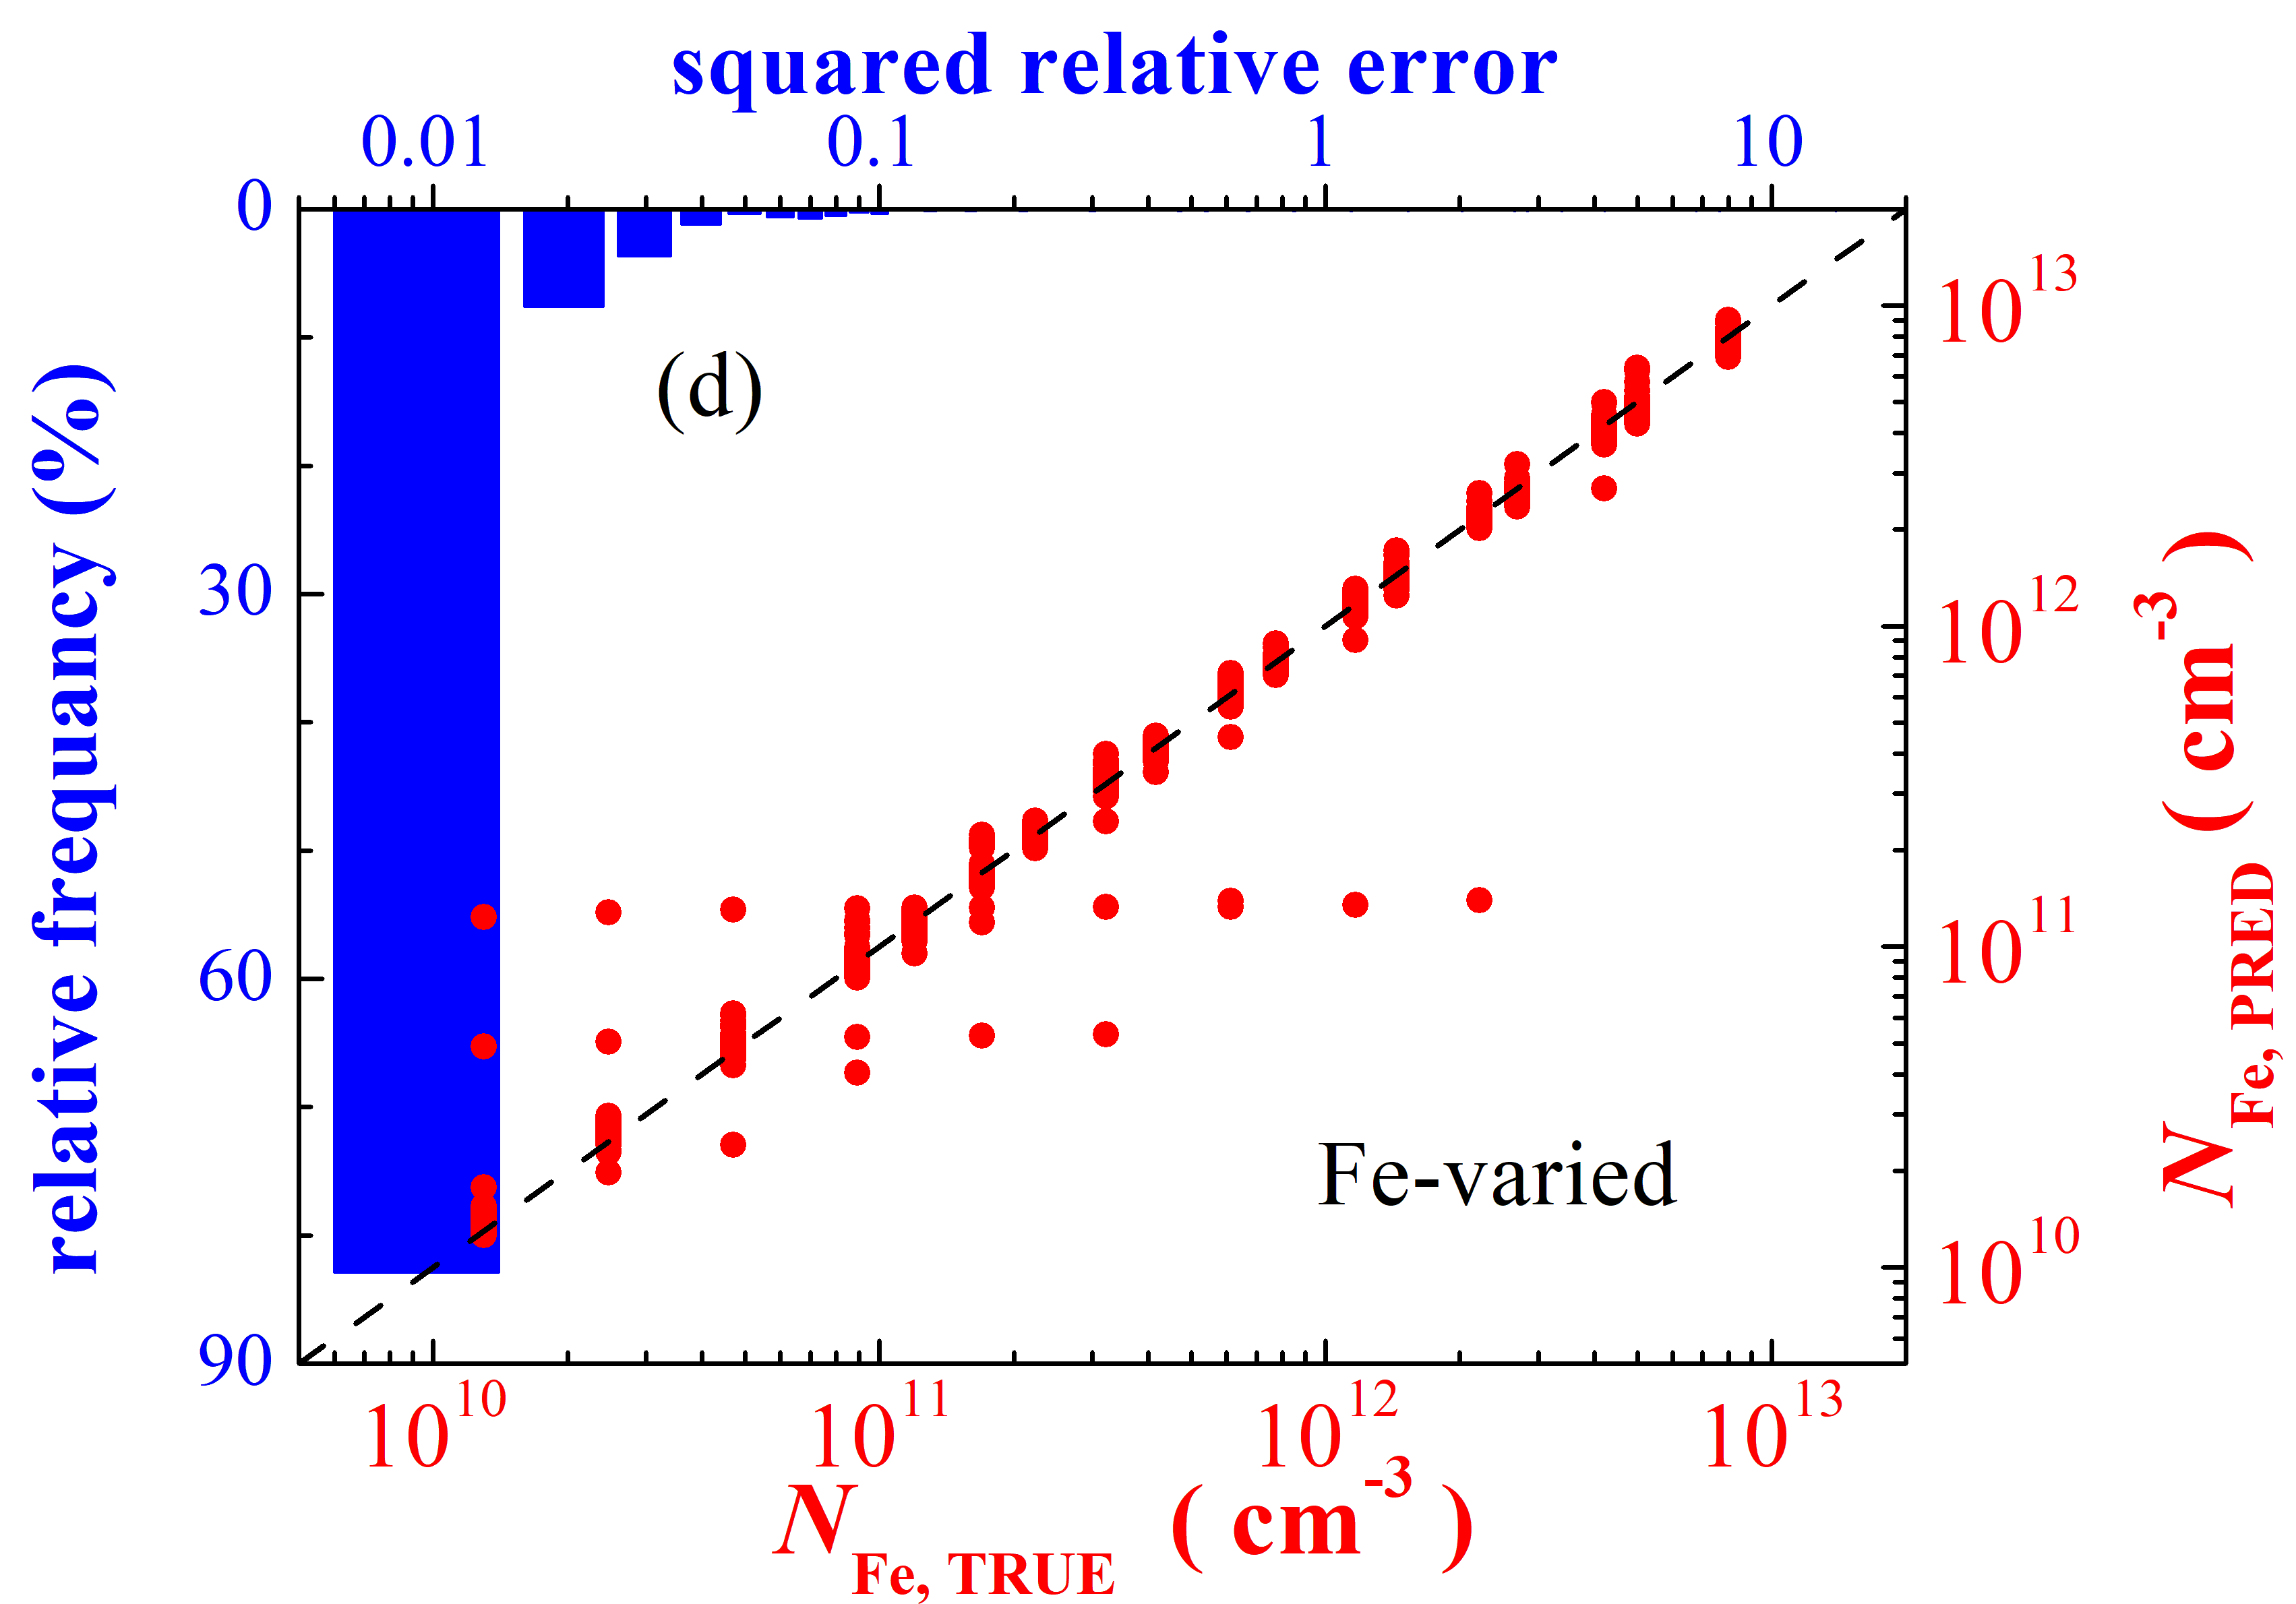
\includegraphics[width=0.32\textwidth]{F3d}
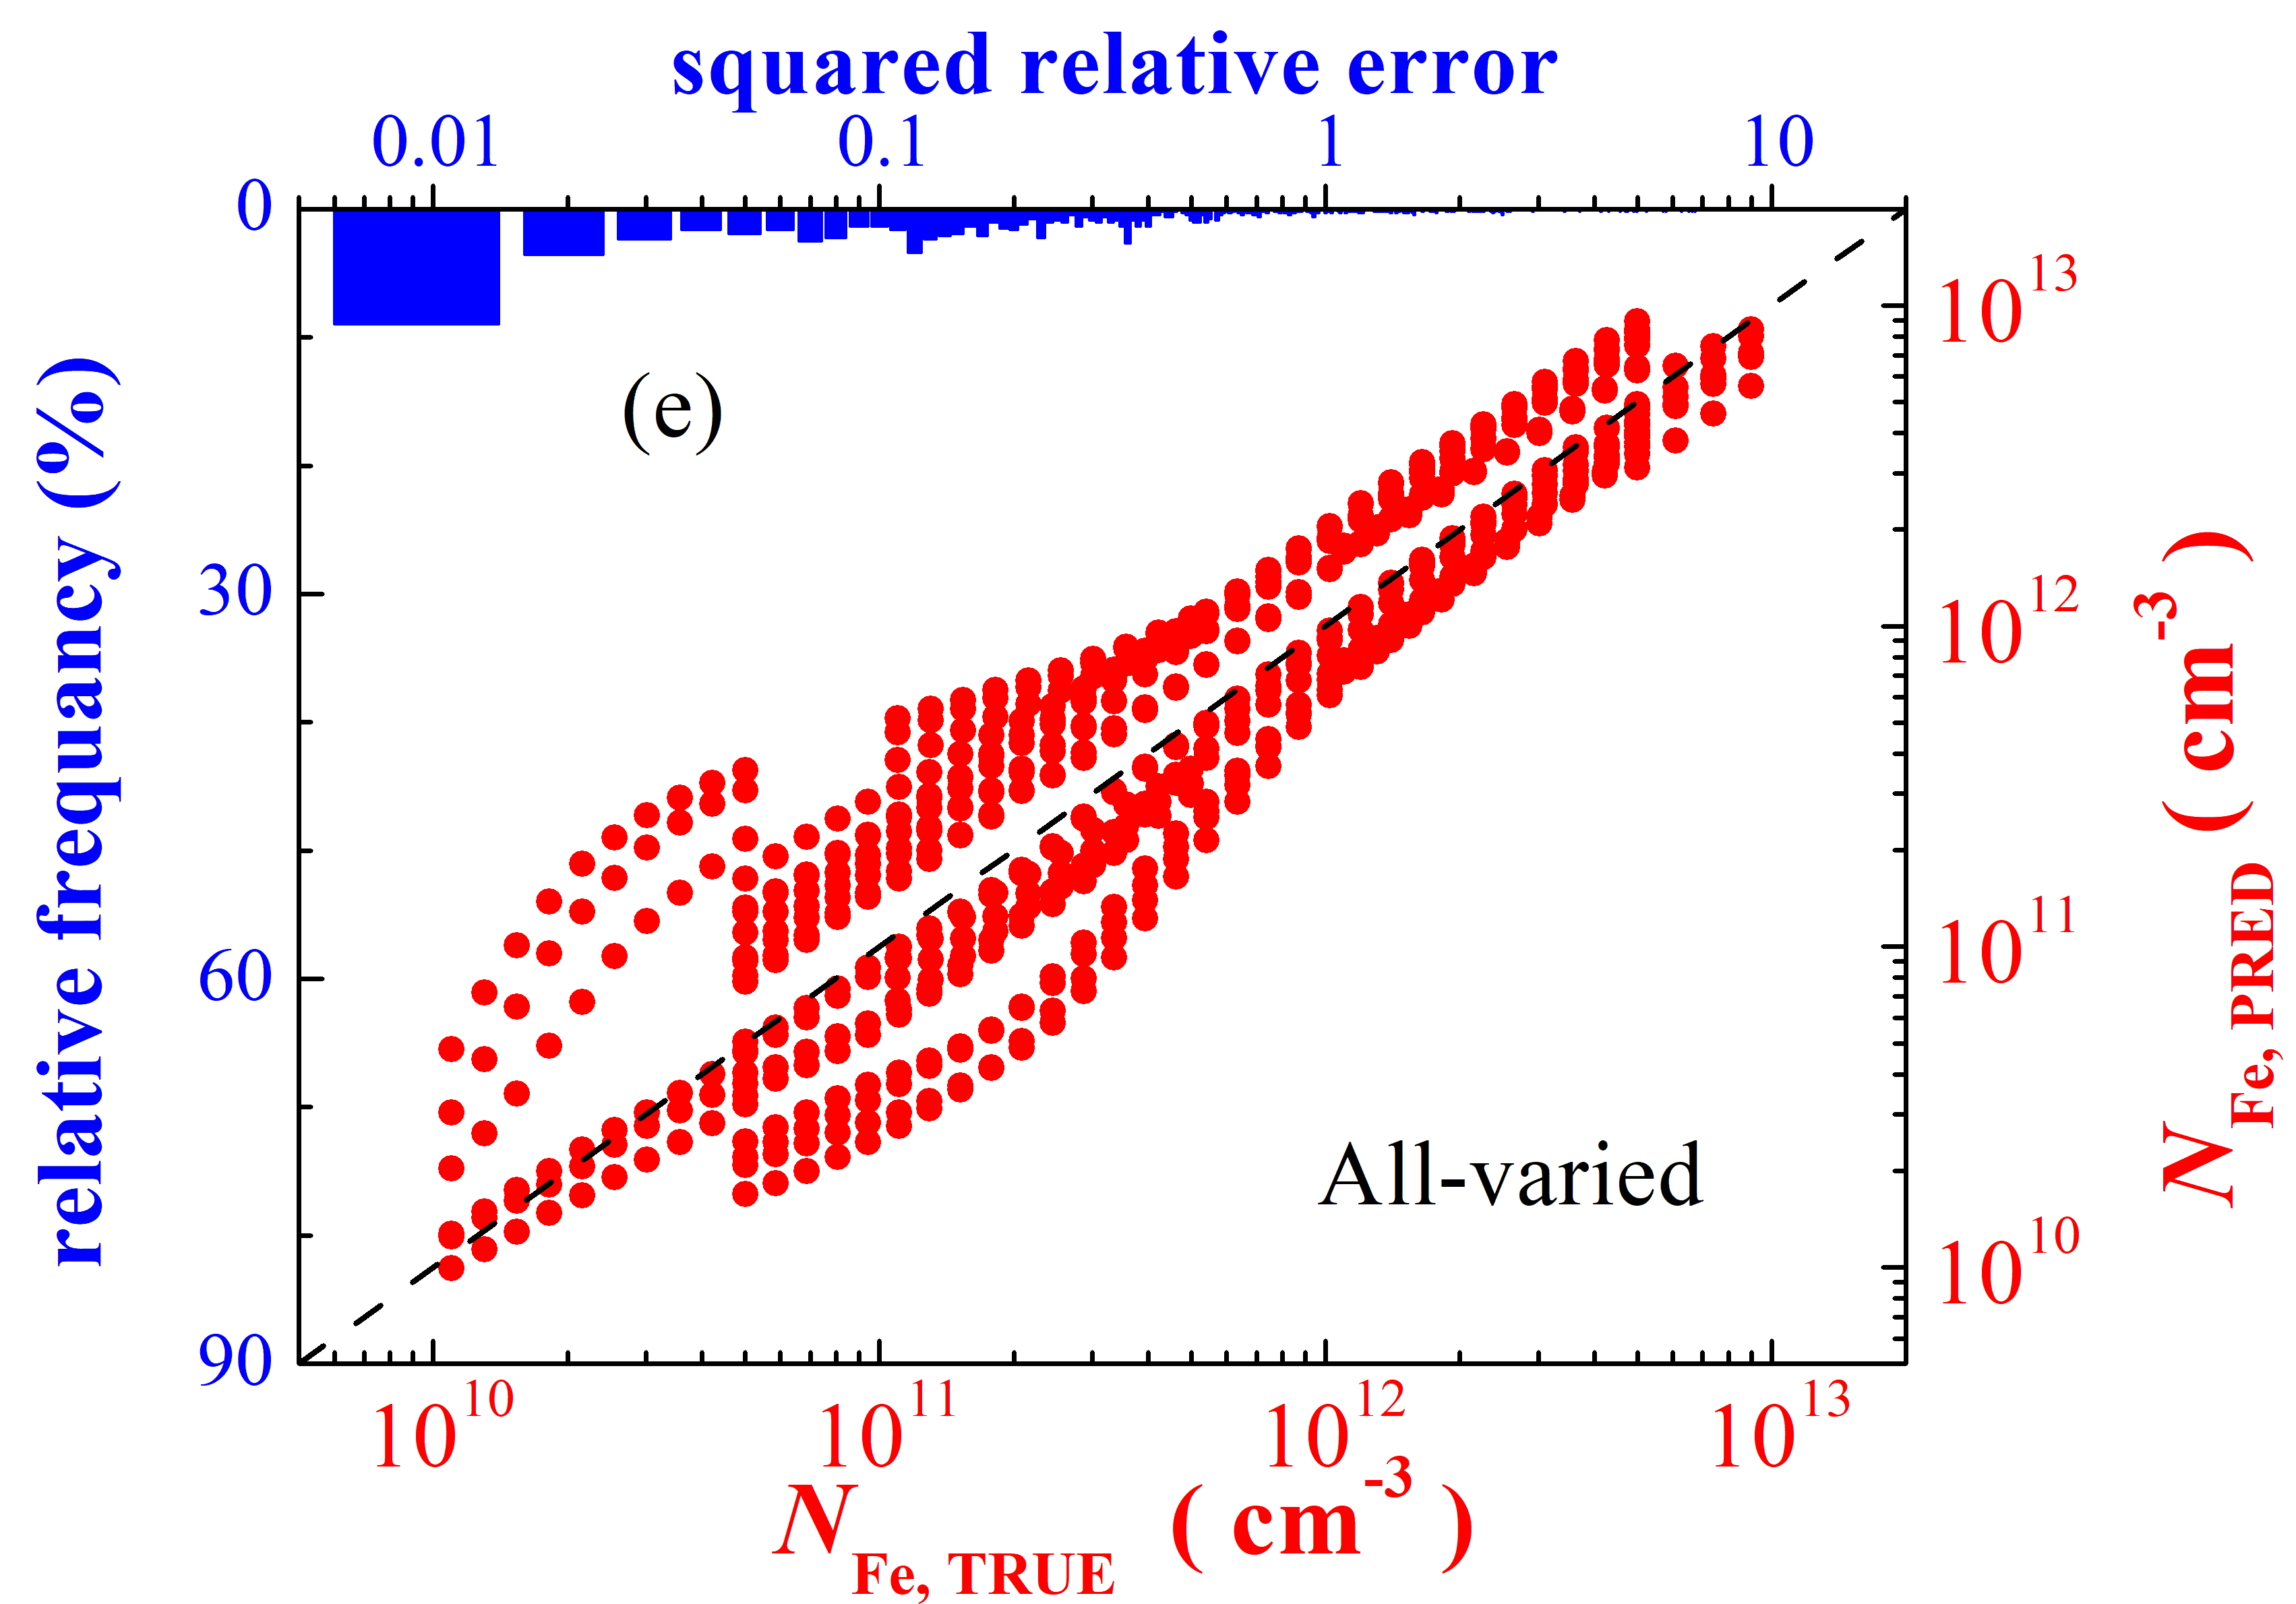
\includegraphics[width=0.32\textwidth]{F3e}
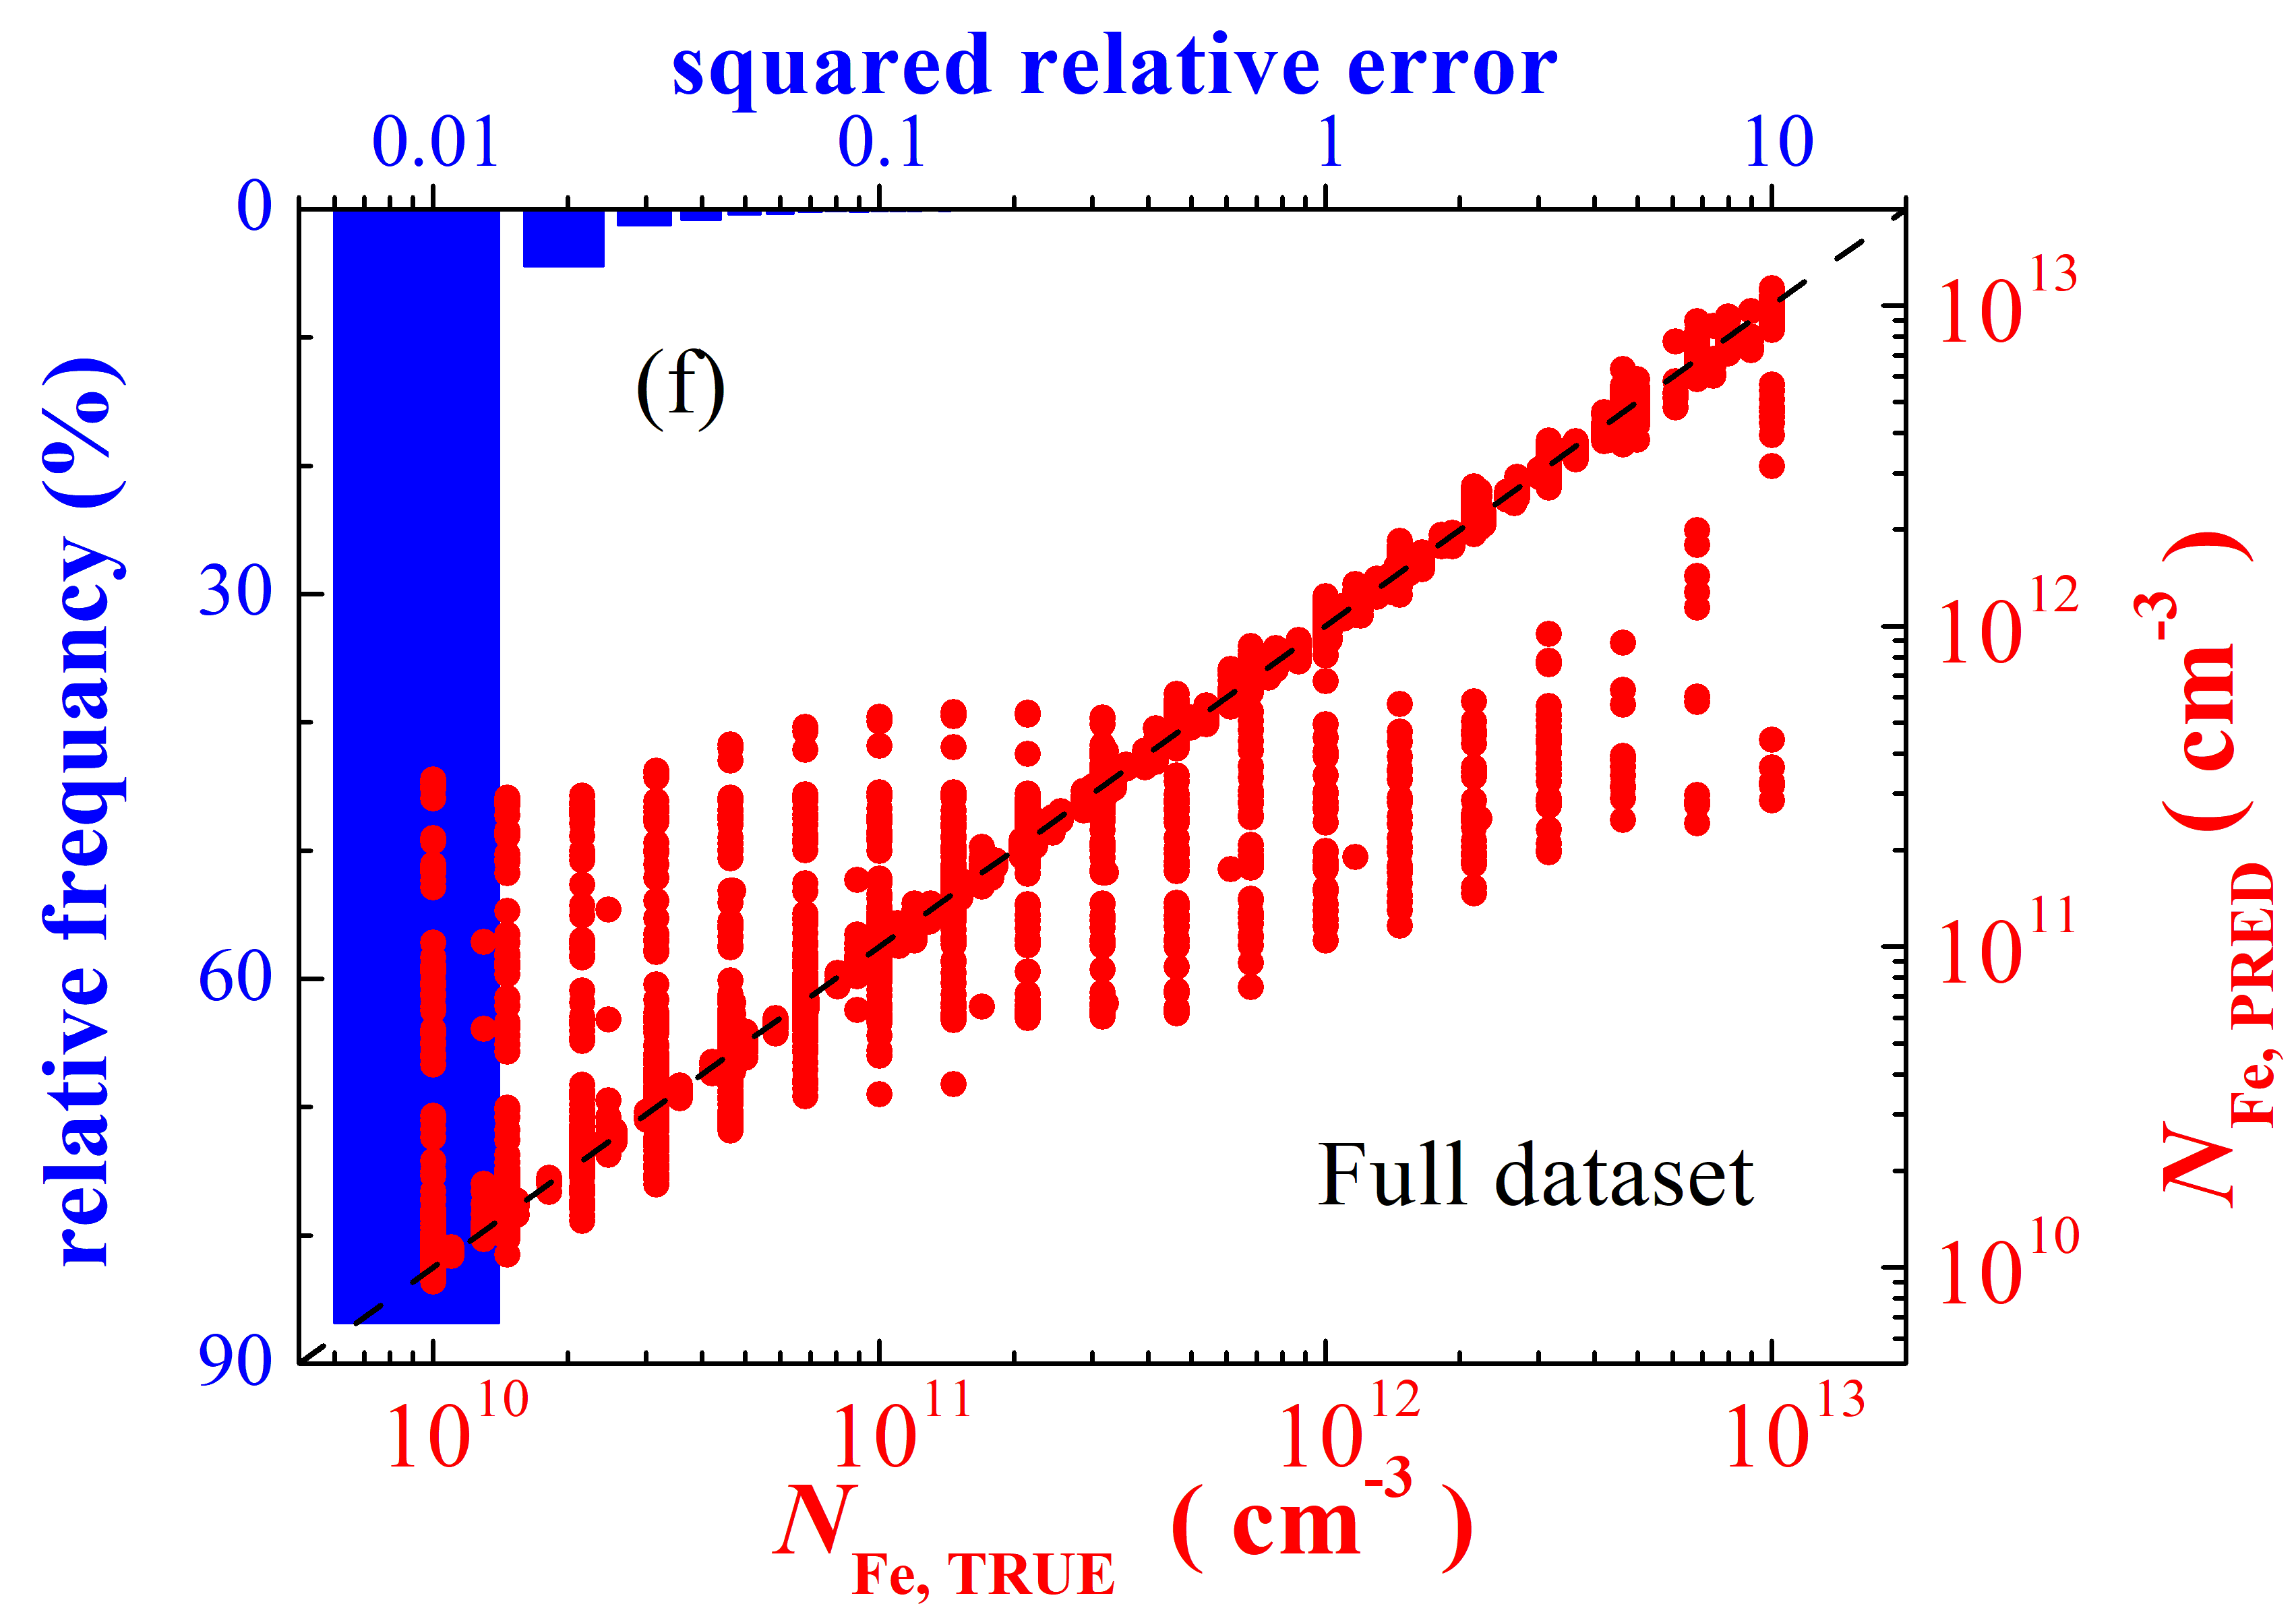
\includegraphics[width=0.32\textwidth]{F3f}
\caption{Iron concentrations are plotted against those generated by DNN$_\mathrm{FeFeB}$
on  T-varied (a),
d-varied (b),
B-varied (c),
Fe-varied (d),
All-varied (e),
and full (f) datasets (red points).
Bars represent histograms of squared relative error.
DNN was learned by training (a)--(e) or full (f) dataset.
The black dashed lines are the identify lines servings as the references.}
\label{fig_TrDNN1}
\end{figure}

The dependencies on DNN prediction error on SC parameters values are under consideration too ---
see Figs.~\ref{fig_Temp}--~\ref{fig_Fe}.
These figures represent data for the training dataset, the results for test datasets are similar.
Thus Fig.~\ref{fig_Temp}(a) shows that the considerable increase in prediction error value is observed at $T>320$~K for DNN$_\mathrm{FeFeB}$.
So the maximum SRE is about 20 and the SRE is less than 0.01 for 55\% of samples at $T=340$~K
(Fig.~\ref{fig_Temp}(c)).
Whereas those values are equal to 0.02 and 83\% at $T=290$~K (Fig.~\ref{fig_Temp}(b)).
It has been shown previously \cite{OlikhJPS}, that temperature rise causes the increase in
the intrinsic recombination's contribution to an ideality factor.
As a result, the sign of Shockley-Read-Hall (SRH) recombination in $n$ value become less evident
and DNN predictive ability falls.

As shown in Fig.~\ref{fig_depth}, the SC base thickness does not influence the prediction error
(mean value as well as relative frequency) practically.
But one can see in Fig~\ref{fig_nValues}(c,d), that an ideality factor value depend on
base thickness at constant $N_\mathrm{Fe}$.
Therefore $d_p$ is a significant parameter for DNN training.

\begin{figure}[tb]
\centering
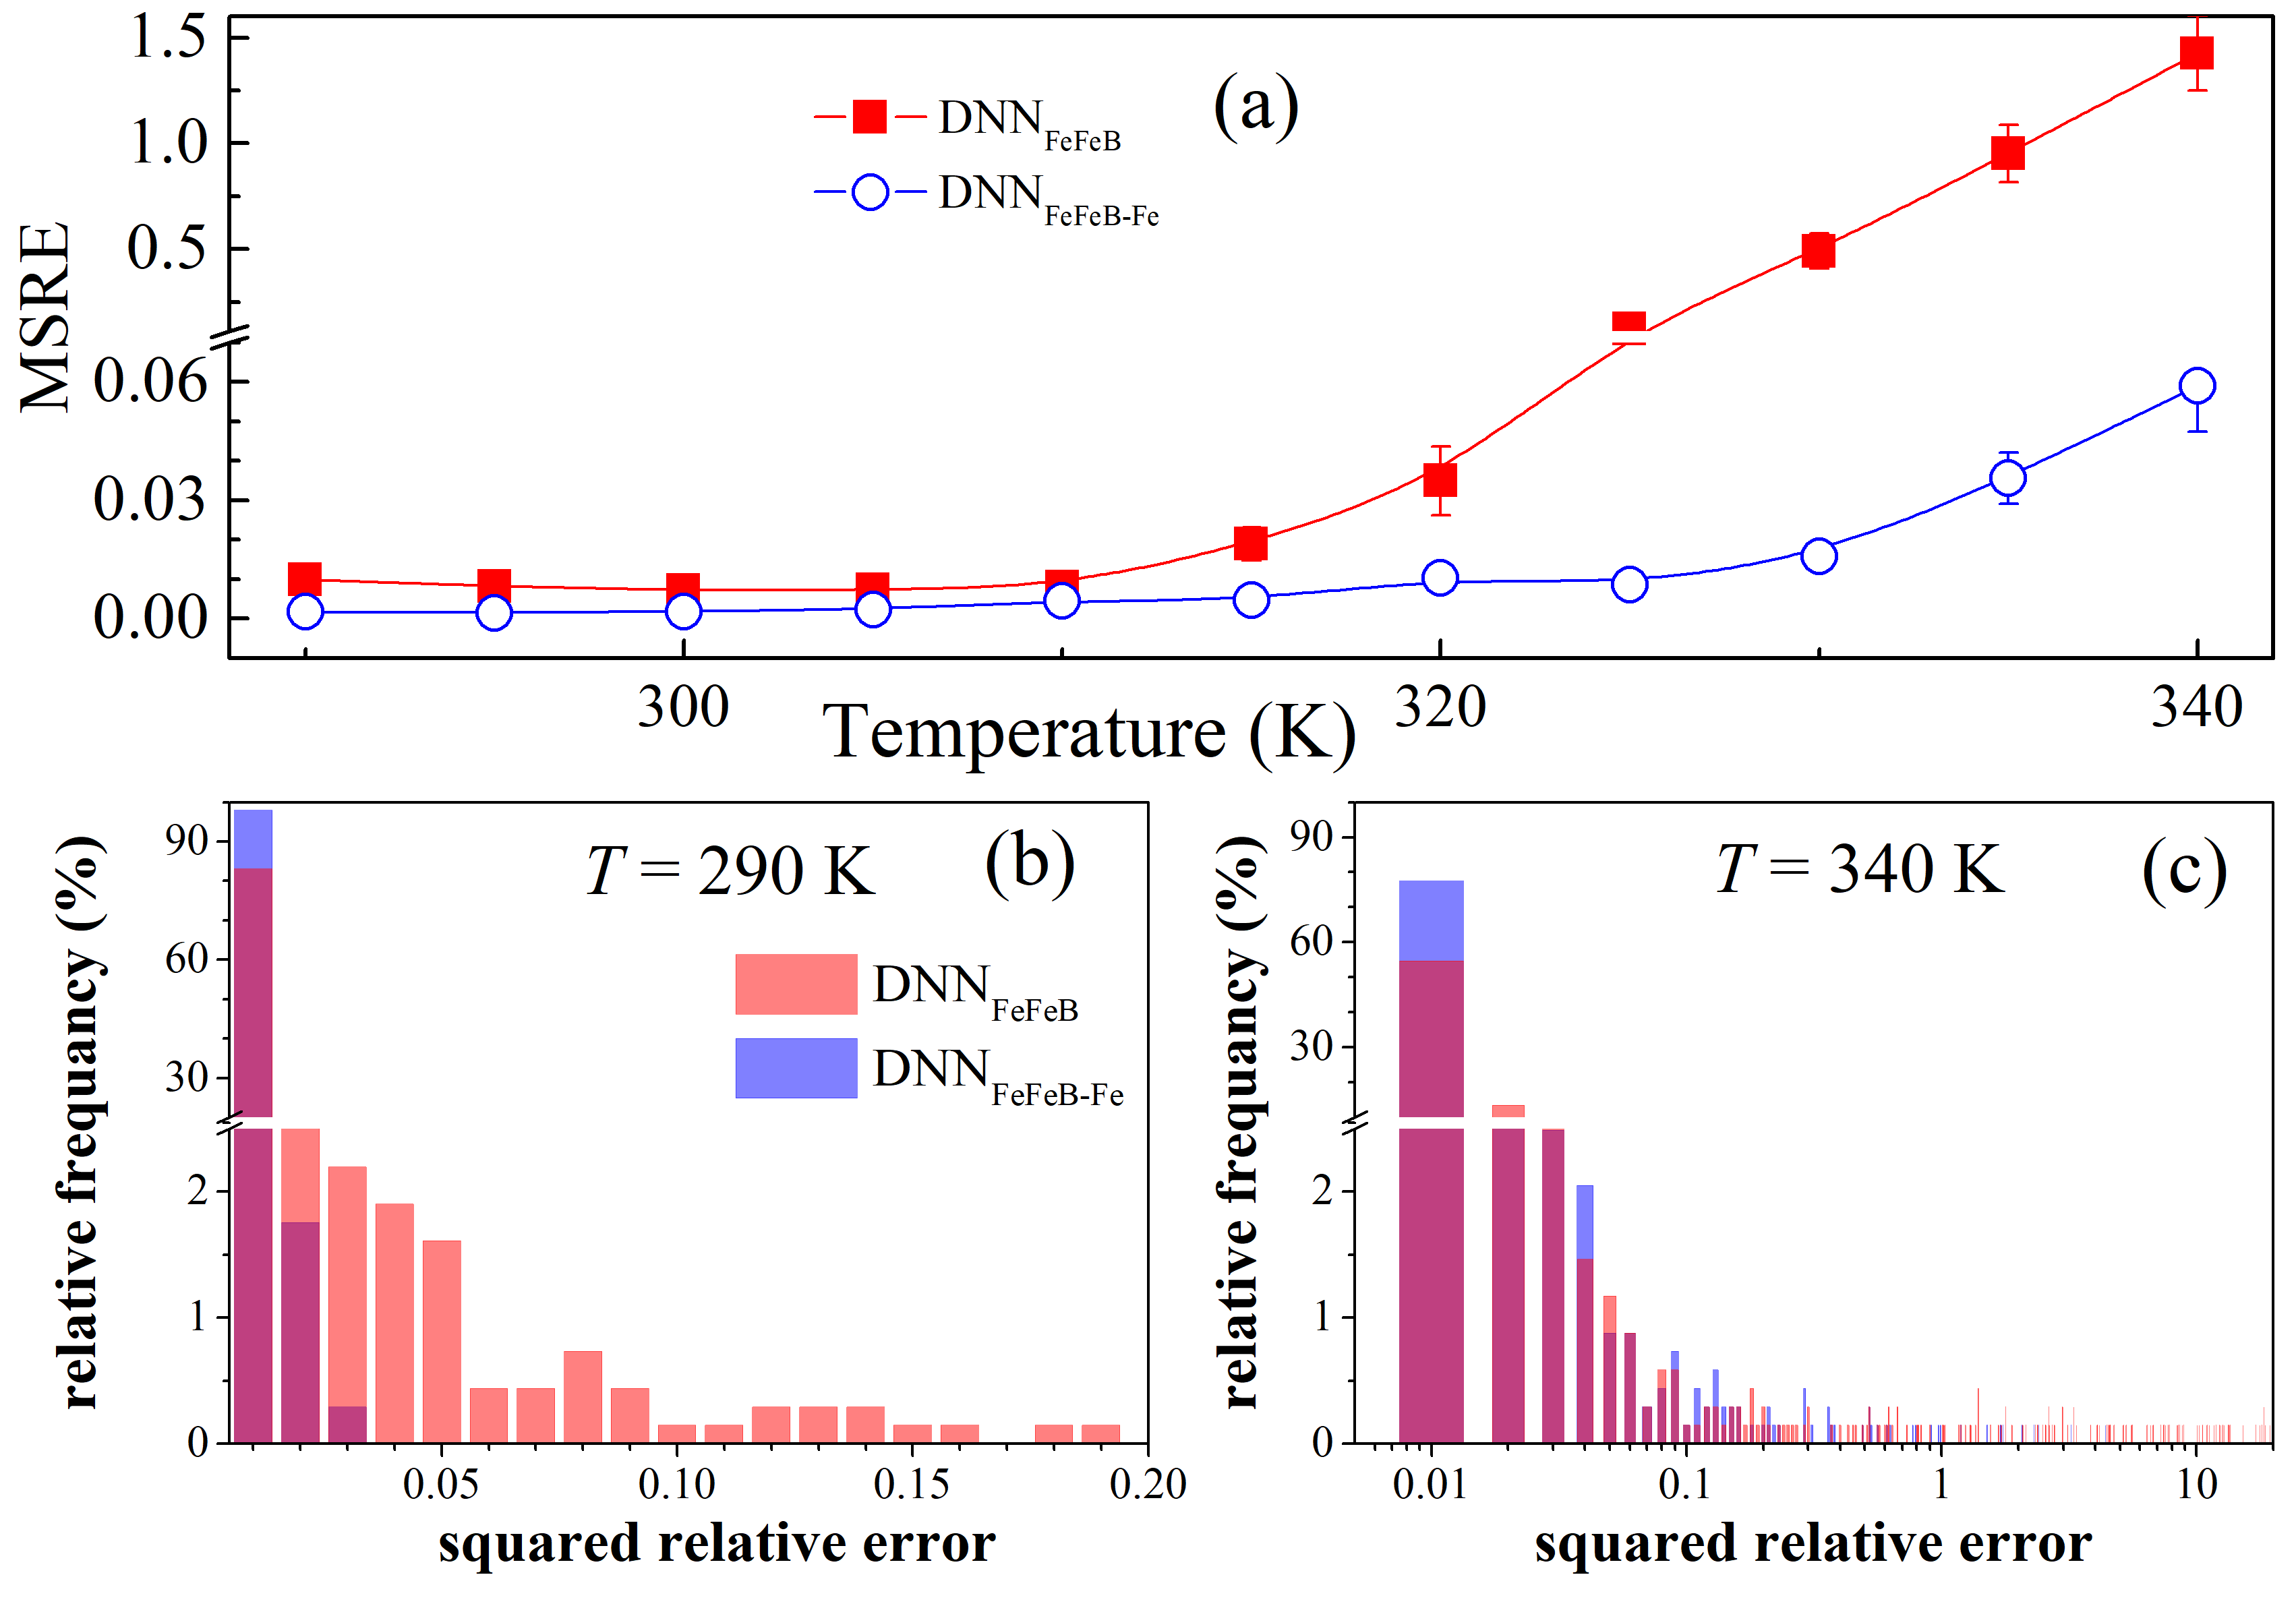
\includegraphics[width=0.48\textwidth]{F4} \hfill
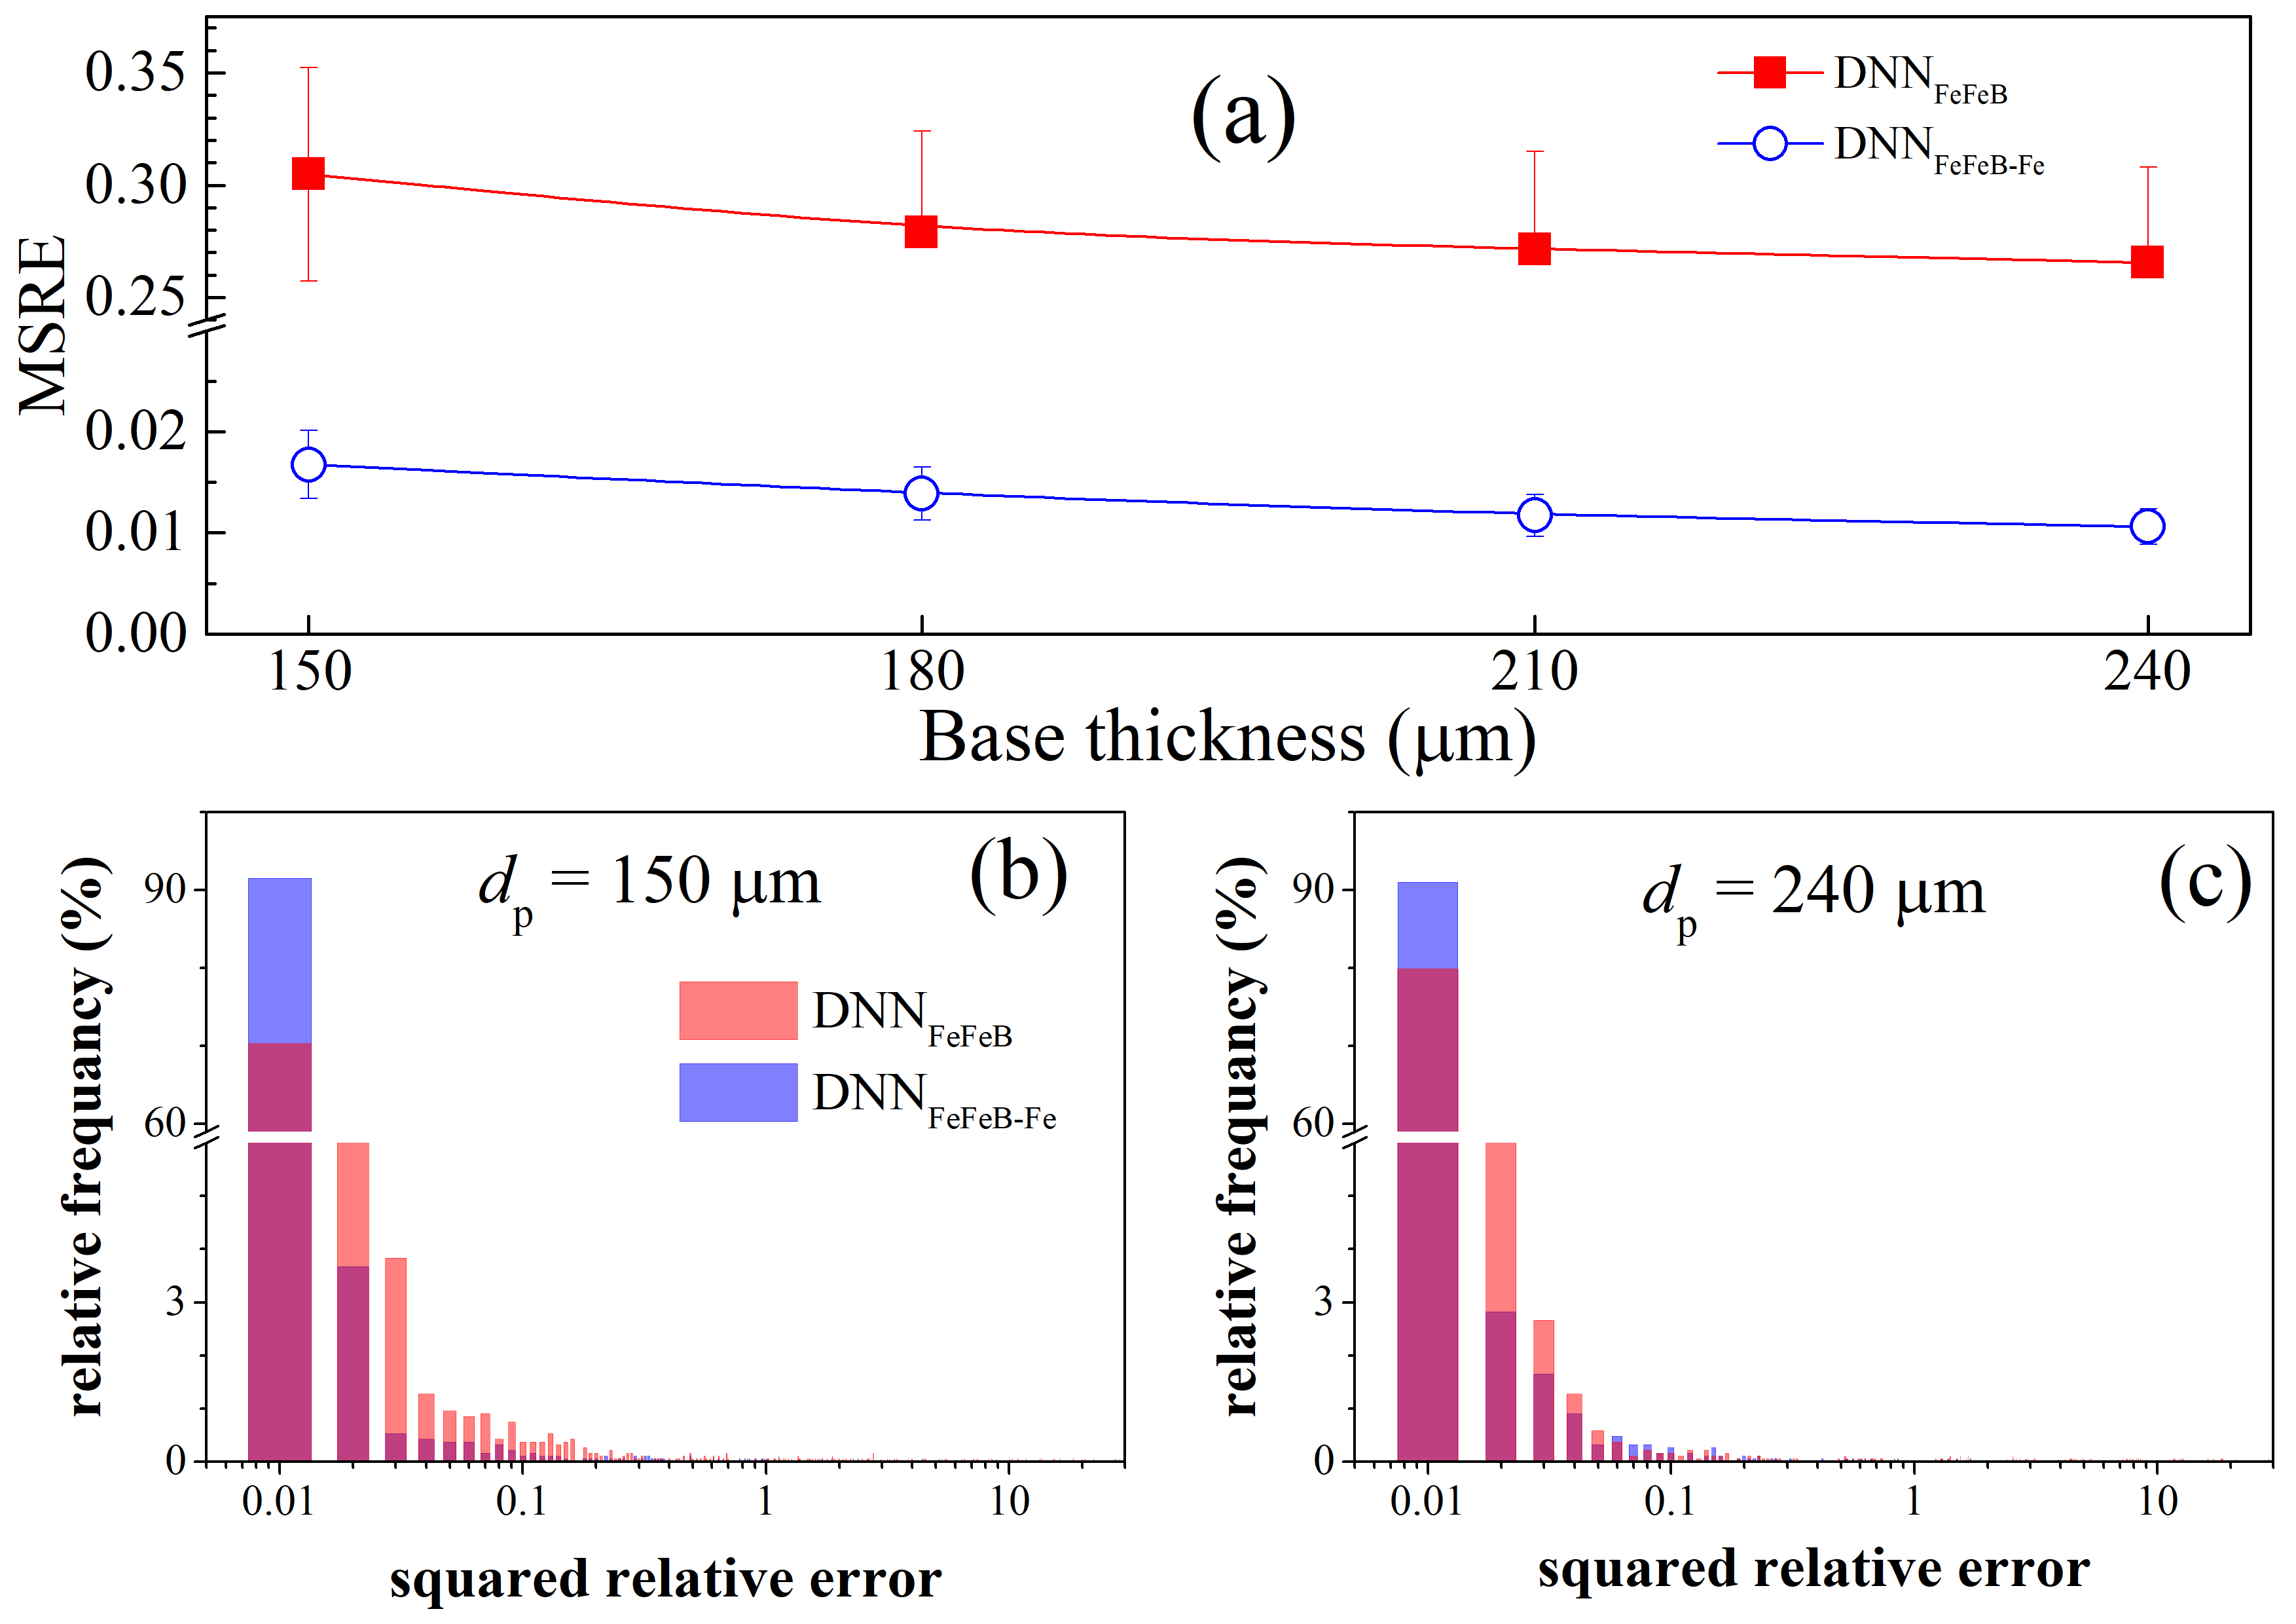
\includegraphics[width=0.48\textwidth]{F5} \\
\parbox[t]{0.48\textwidth}
{\caption{(a) Dependence of the MSRE (training dataset) on the temperature.
(b),(c) Histograms of squared relative error for $T=290$~K and $T=340$~K.
Red: DNN$_\mathrm{FeFeB}$; blue: DNN$_\mathrm{FeFeB-Fe}$.
}
\label{fig_Temp}} \hfill
\parbox[t]{0.48\textwidth}{\caption{(a) Dependence of the MSRE (training dataset) on the base thickness.
(b),(c) Histograms of squared relative error for $d_p=150$~$\mu$m and $d_p=240$~$\mu$m.
Red: DNN$_\mathrm{FeFeB}$; blue: DNN$_\mathrm{FeFeB-Fe}$.}
\label{fig_depth}}
\end{figure}

The predictive error rises sharply with doping level decrees --- see Fig.~\ref{fig_B}(a).
Thus maximum SRE is about 0.05 for $N_\mathrm{B}=10^{17}$~cm$^{-3}$ (Fig.~\ref{fig_B}(c))
whereas squared relative error is less than 0.05 for 56\% of samples only
for $N_\mathrm{B}=10^{15}$~cm$^{-3}$ (Fig.~\ref{fig_B}(b)).
The hole occupation of the Fe-related level determines the SRH recombination efficiency.
Accordingly to the Fermi-Dirac statistics, the probability of a hole
occupation in a non-degenerate $p$-type semiconductor with full acceptor depletion can be expressed as
\begin{equation}
\label{eqfp}
 f_p=\frac{1}{1+\frac{N_V}{N_\mathrm{B}}\exp\left(\frac{E_V-E_{\mathrm{Fe}_i}}{kT}\right)}\,.
\end{equation}
If $N_\mathrm{B}$ decreases, the level is filled with an electron,
the SRH recombination ceases, and the ideality factor value sharply reduces  --- Fig.~\ref{fig_nValues}(a,b).
Besides, a weak influence of impurities on ideality factor under low doping conditions is a reason
for observed MSRE increase.
In our opinion, the level filling is an additional reason for an error increase at high temperatures as well.


\begin{figure}[tb]
\centering
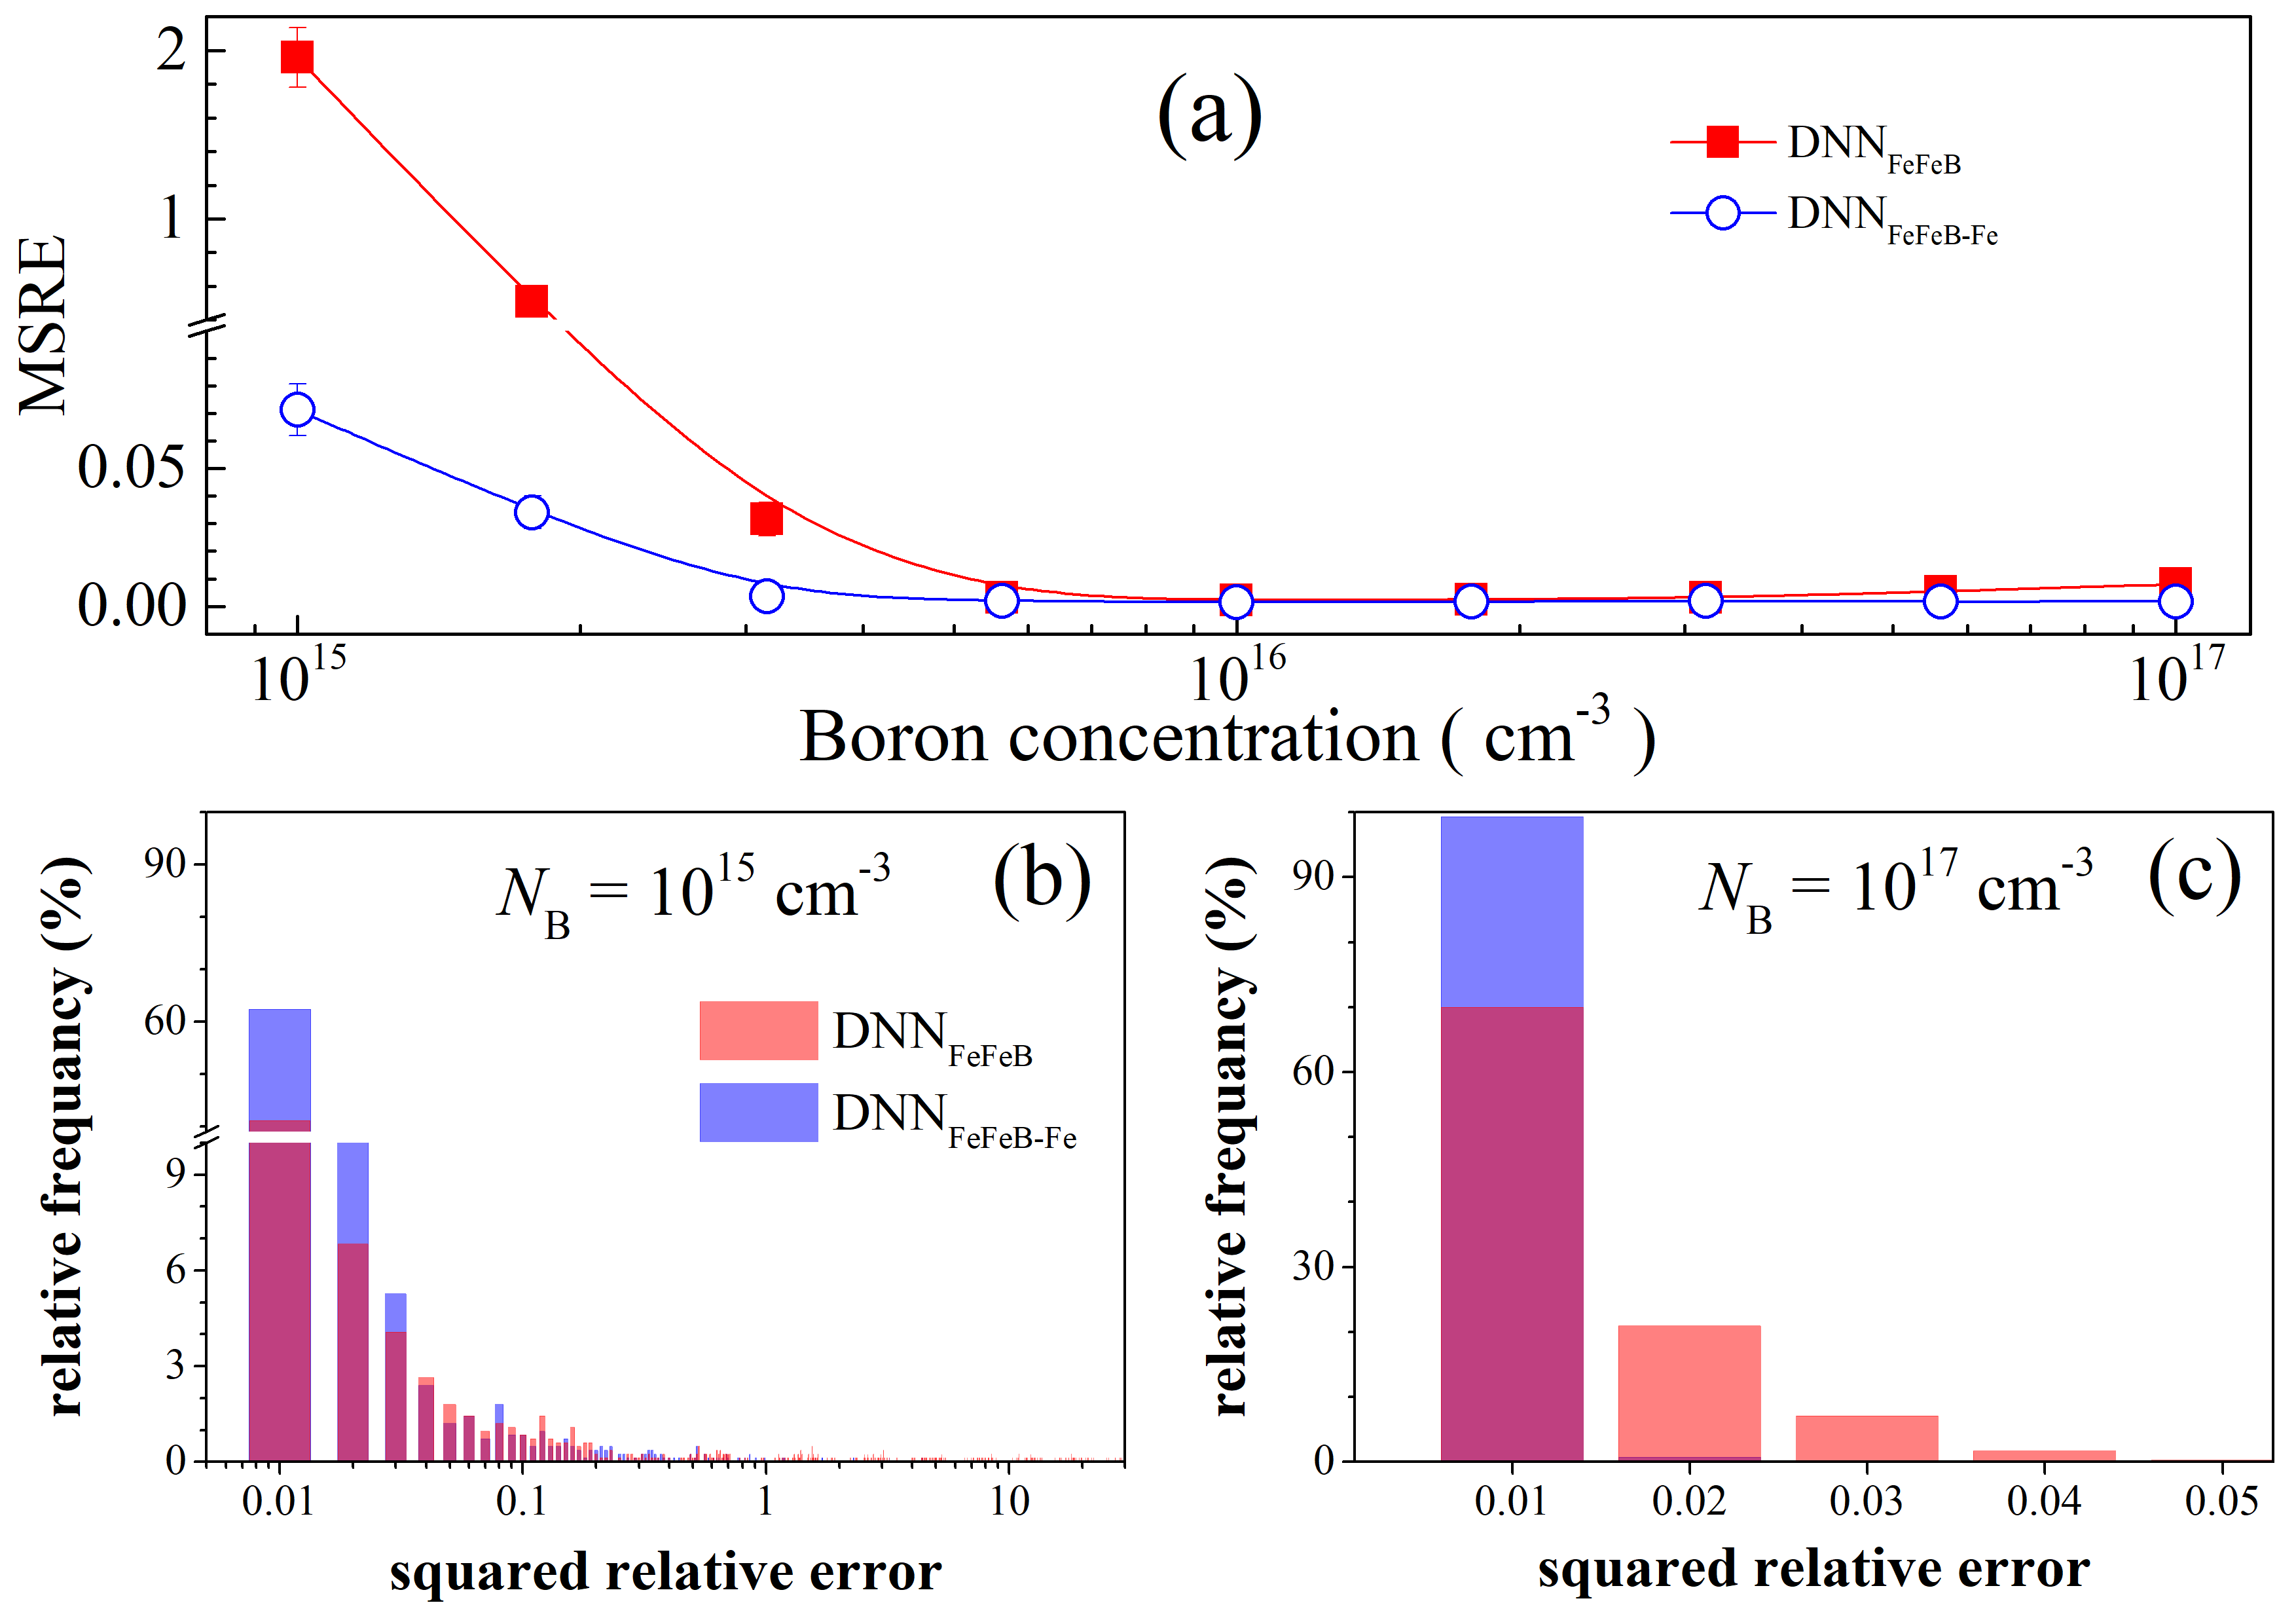
\includegraphics[width=0.48\textwidth]{F6} \hfill
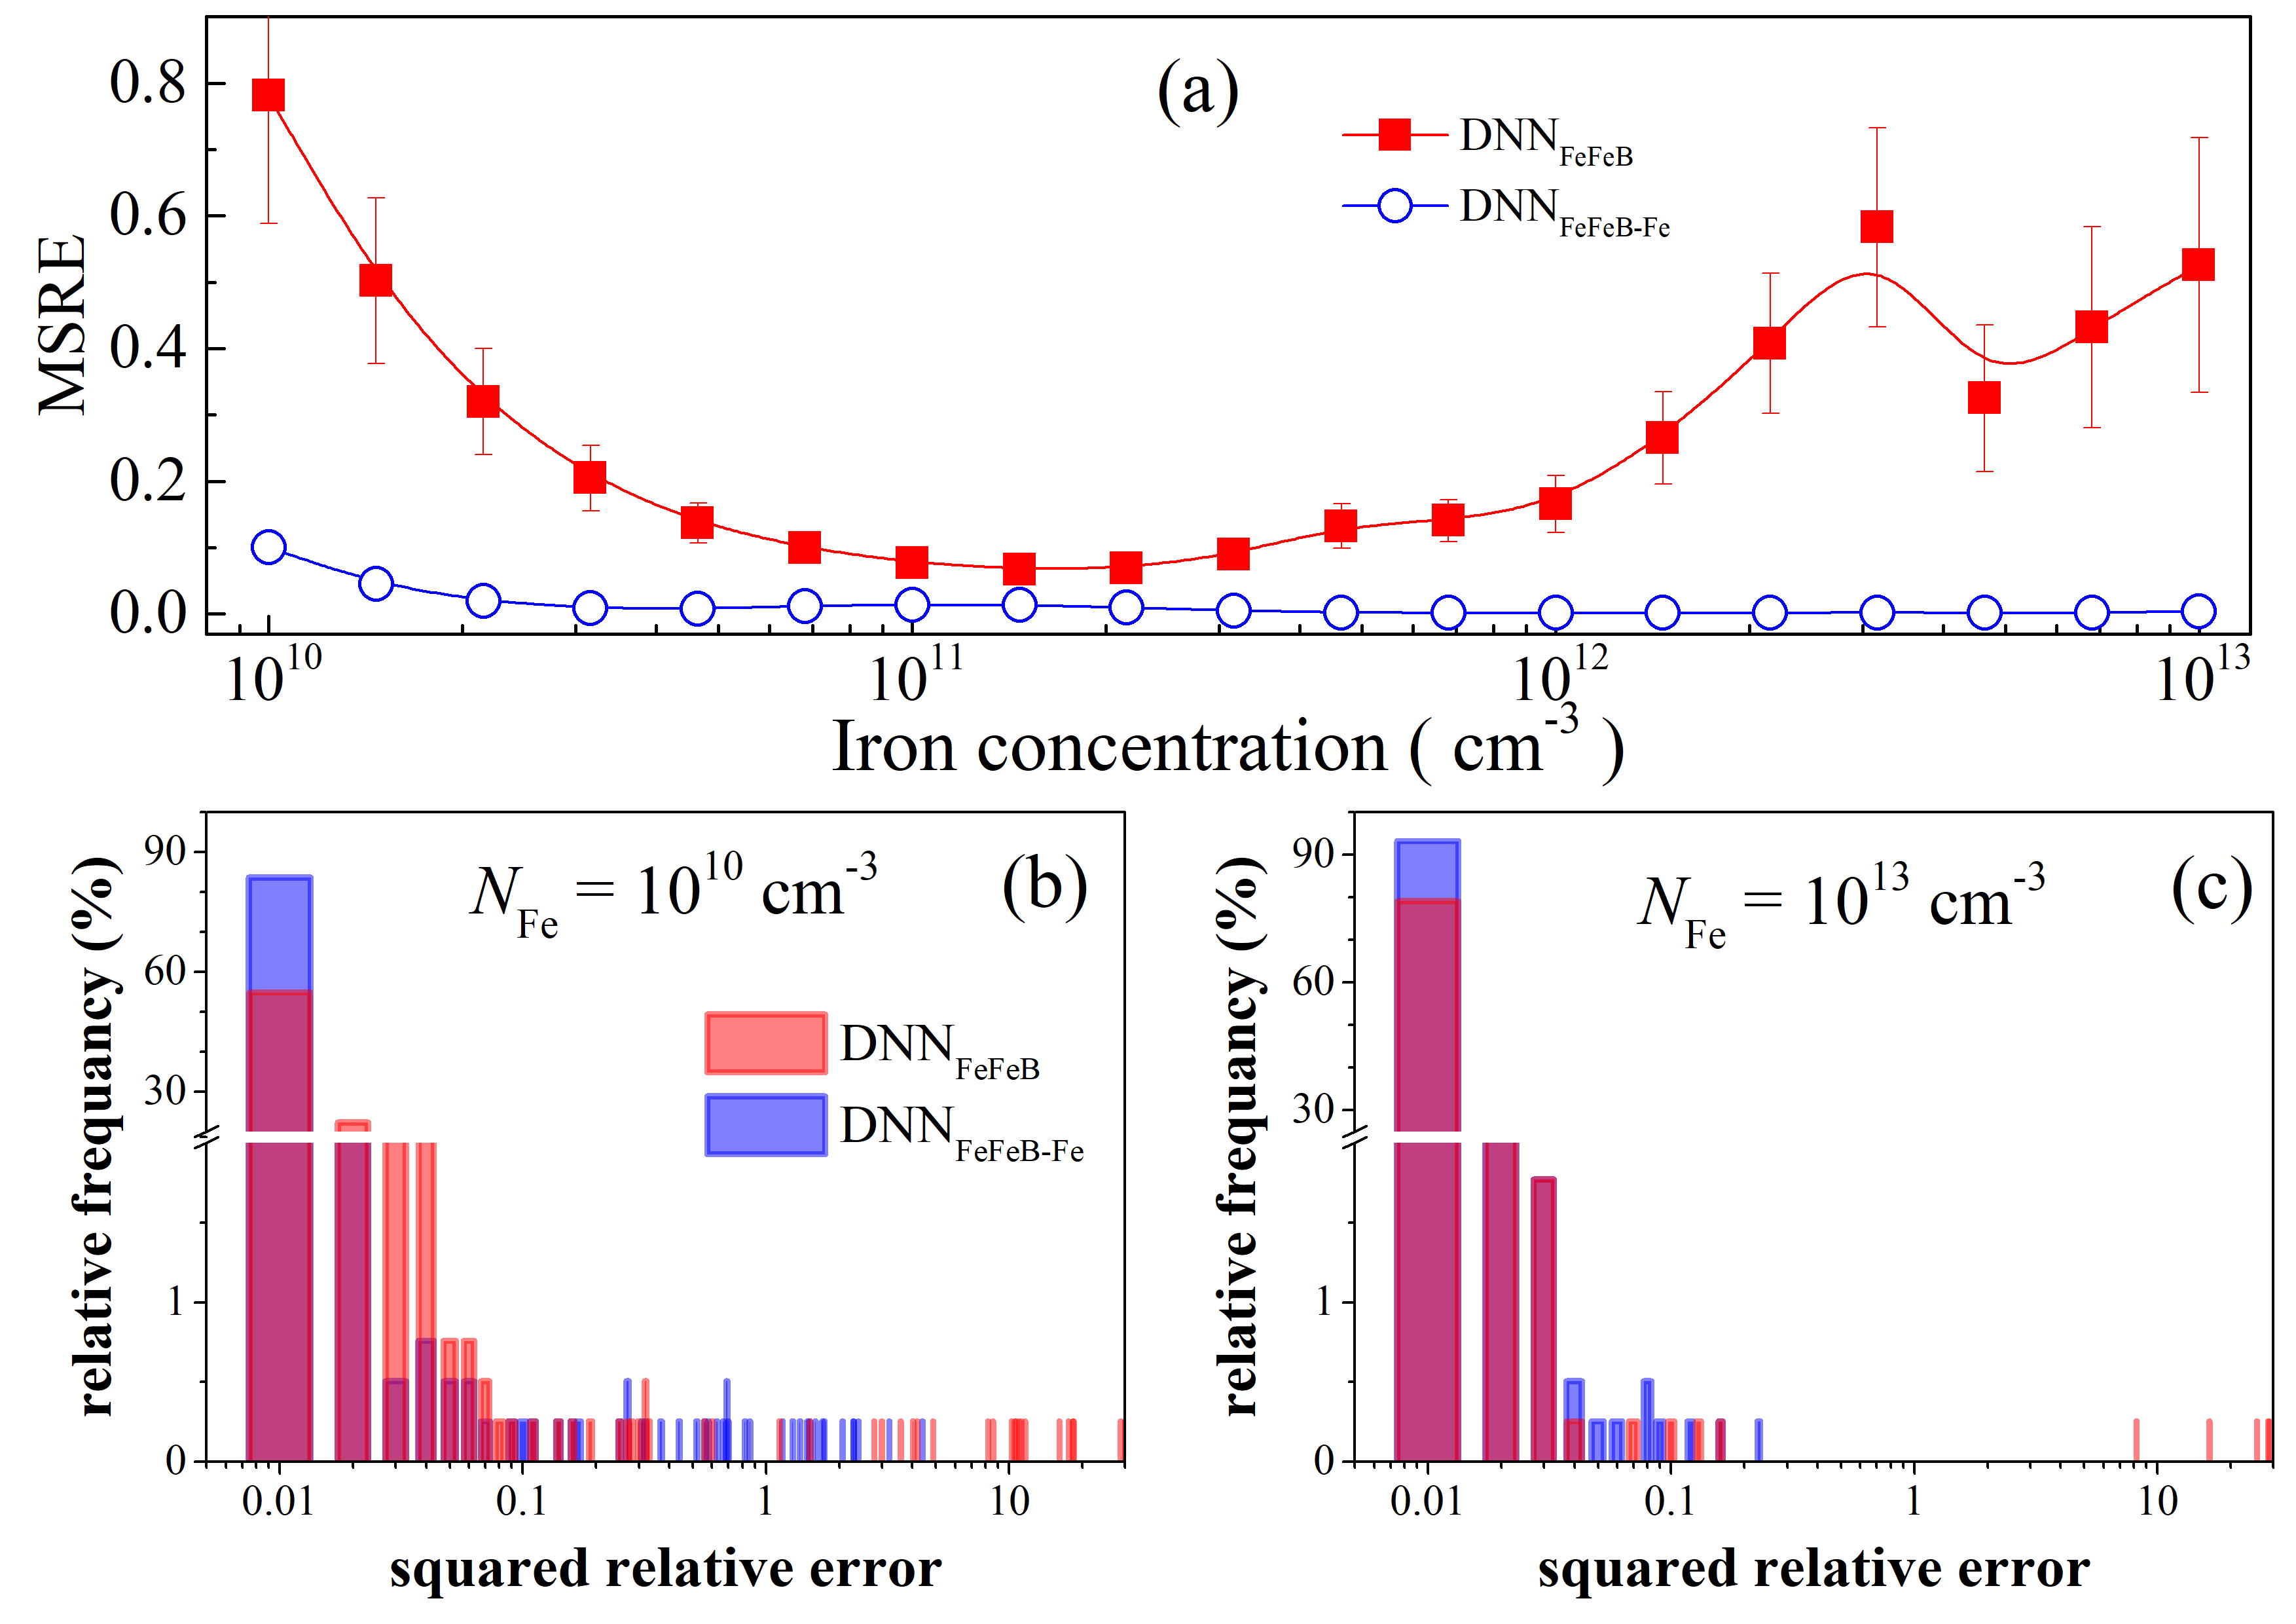
\includegraphics[width=0.48\textwidth]{F7} \\
\parbox[t]{0.48\textwidth}
{\caption{(a) Dependence of the MSRE (training dataset) on the boron concentration.
(b),(c) Histograms of squared  relative error for $N_\mathrm{B}=10^{15}$~cm$^{-3}$ and $N_\mathrm{B}=10^{17}$~cm$^{-3}$.
Red: DNN$_\mathrm{FeFeB}$; blue: DNN$_\mathrm{FeFeB-Fe}$.
}
\label{fig_B}} \hfill
\parbox[t]{0.48\textwidth}{\caption{(a) Dependence of the MSRE (training dataset) on the iron concentration.
(b),(c) Histograms of squared  relative error for $N_\mathrm{Fe}=10^{10}$~cm$^{-3}$ and $N_\mathrm{Fe}=10^{13}$~cm$^{-3}$.
Red: DNN$_\mathrm{FeFeB}$; blue: DNN$_\mathrm{FeFeB-Fe}$.}
\label{fig_Fe}}
\end{figure}

Fig.~\ref{fig_Fe}(a) shows that MSRE increases at both low and high iron concentrations.
The first $N_\mathrm{Fe}$ area of bad DNN accuracy is entirely  foreseeable,
the second one is surprising enough.
But accordingly to Fig~\ref{fig_Fe}(c), the MSRE increasing at $N_\mathrm{Fe}=10^{13}$~cm$^{-3}$ is most likely determined by  a few samples with big SRE value.
Whereas SRE increasing is more systematic at $N_\mathrm{Fe}=10^{13}$~cm$^{-3}$ --- Fig~\ref{fig_Fe}(b).

The ideality factor value for the case of interstitial iron only presence ($n_\mathrm{Fe}$)
gives additional information about defects in comparing with $n_\mathrm{Fe-FeB}$.
It is not surprising that DNN$_\mathrm{FeFeB-Fe}$ has better operating parameters in comparing with
DNN$_\mathrm{FeFeB}$ --- see Table~\ref{table_CV}, Table~\ref{table_MSRE}, Fig.~\ref{fig_TrDNN2}.
The operation improvement appearances in the MSRE decrease as well as in
absence of huge difference between $N_\mathrm{Fe,TRUE}$ and $N_\mathrm{Fe,PRED}$ values
and narrowing of SRE range (Figs.~\ref{fig_Temp}-\ref{fig_TrDNN2}).
Really, it is shown in Fig.~\ref{fig_TrDNN2} that the maximum SRE does not exceed one even in the case of All-varied datasets
and SRE is less than 0.02 for 93\%, 92\%, 73\%, and 97\% of samples of T-varied, d-varied, B-varied, and Fe-varied datasets respectively.
The $R^2$ (0.999) and $R$ (0.999) values for Fe-varied dataset draws attention as well.

\begin{figure}[tb]
\centering
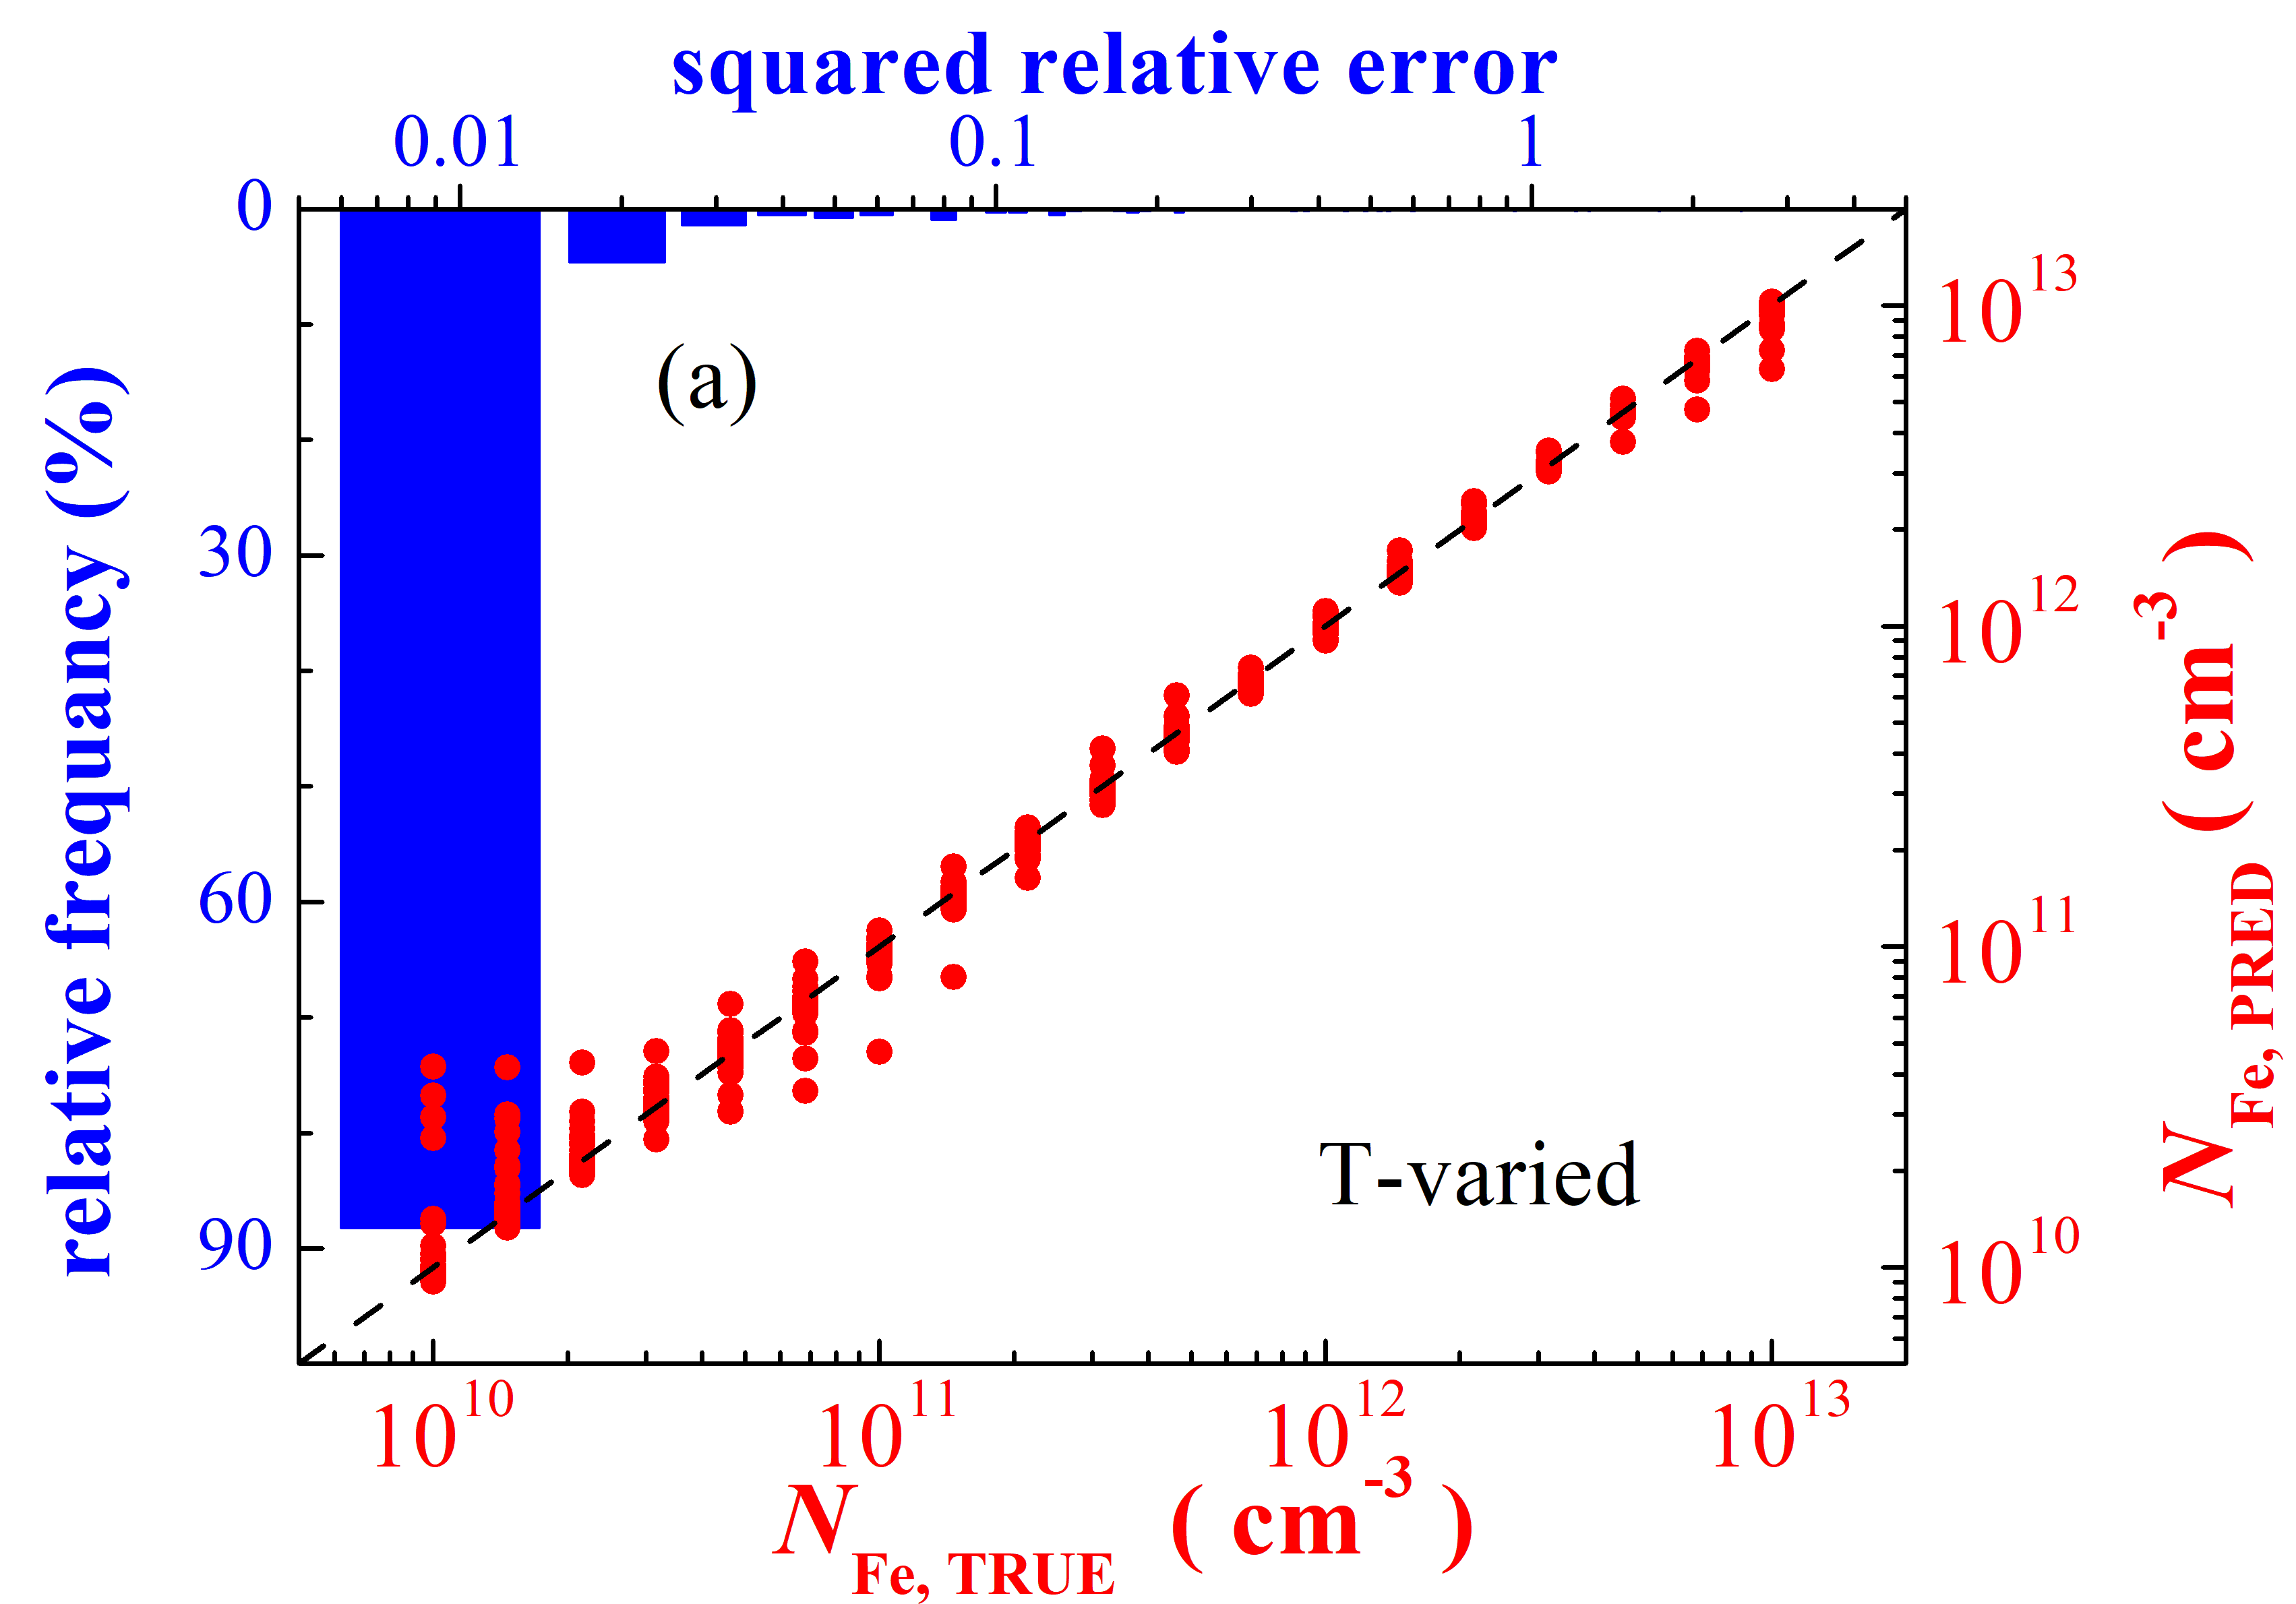
\includegraphics[width=0.32\textwidth]{F8a}
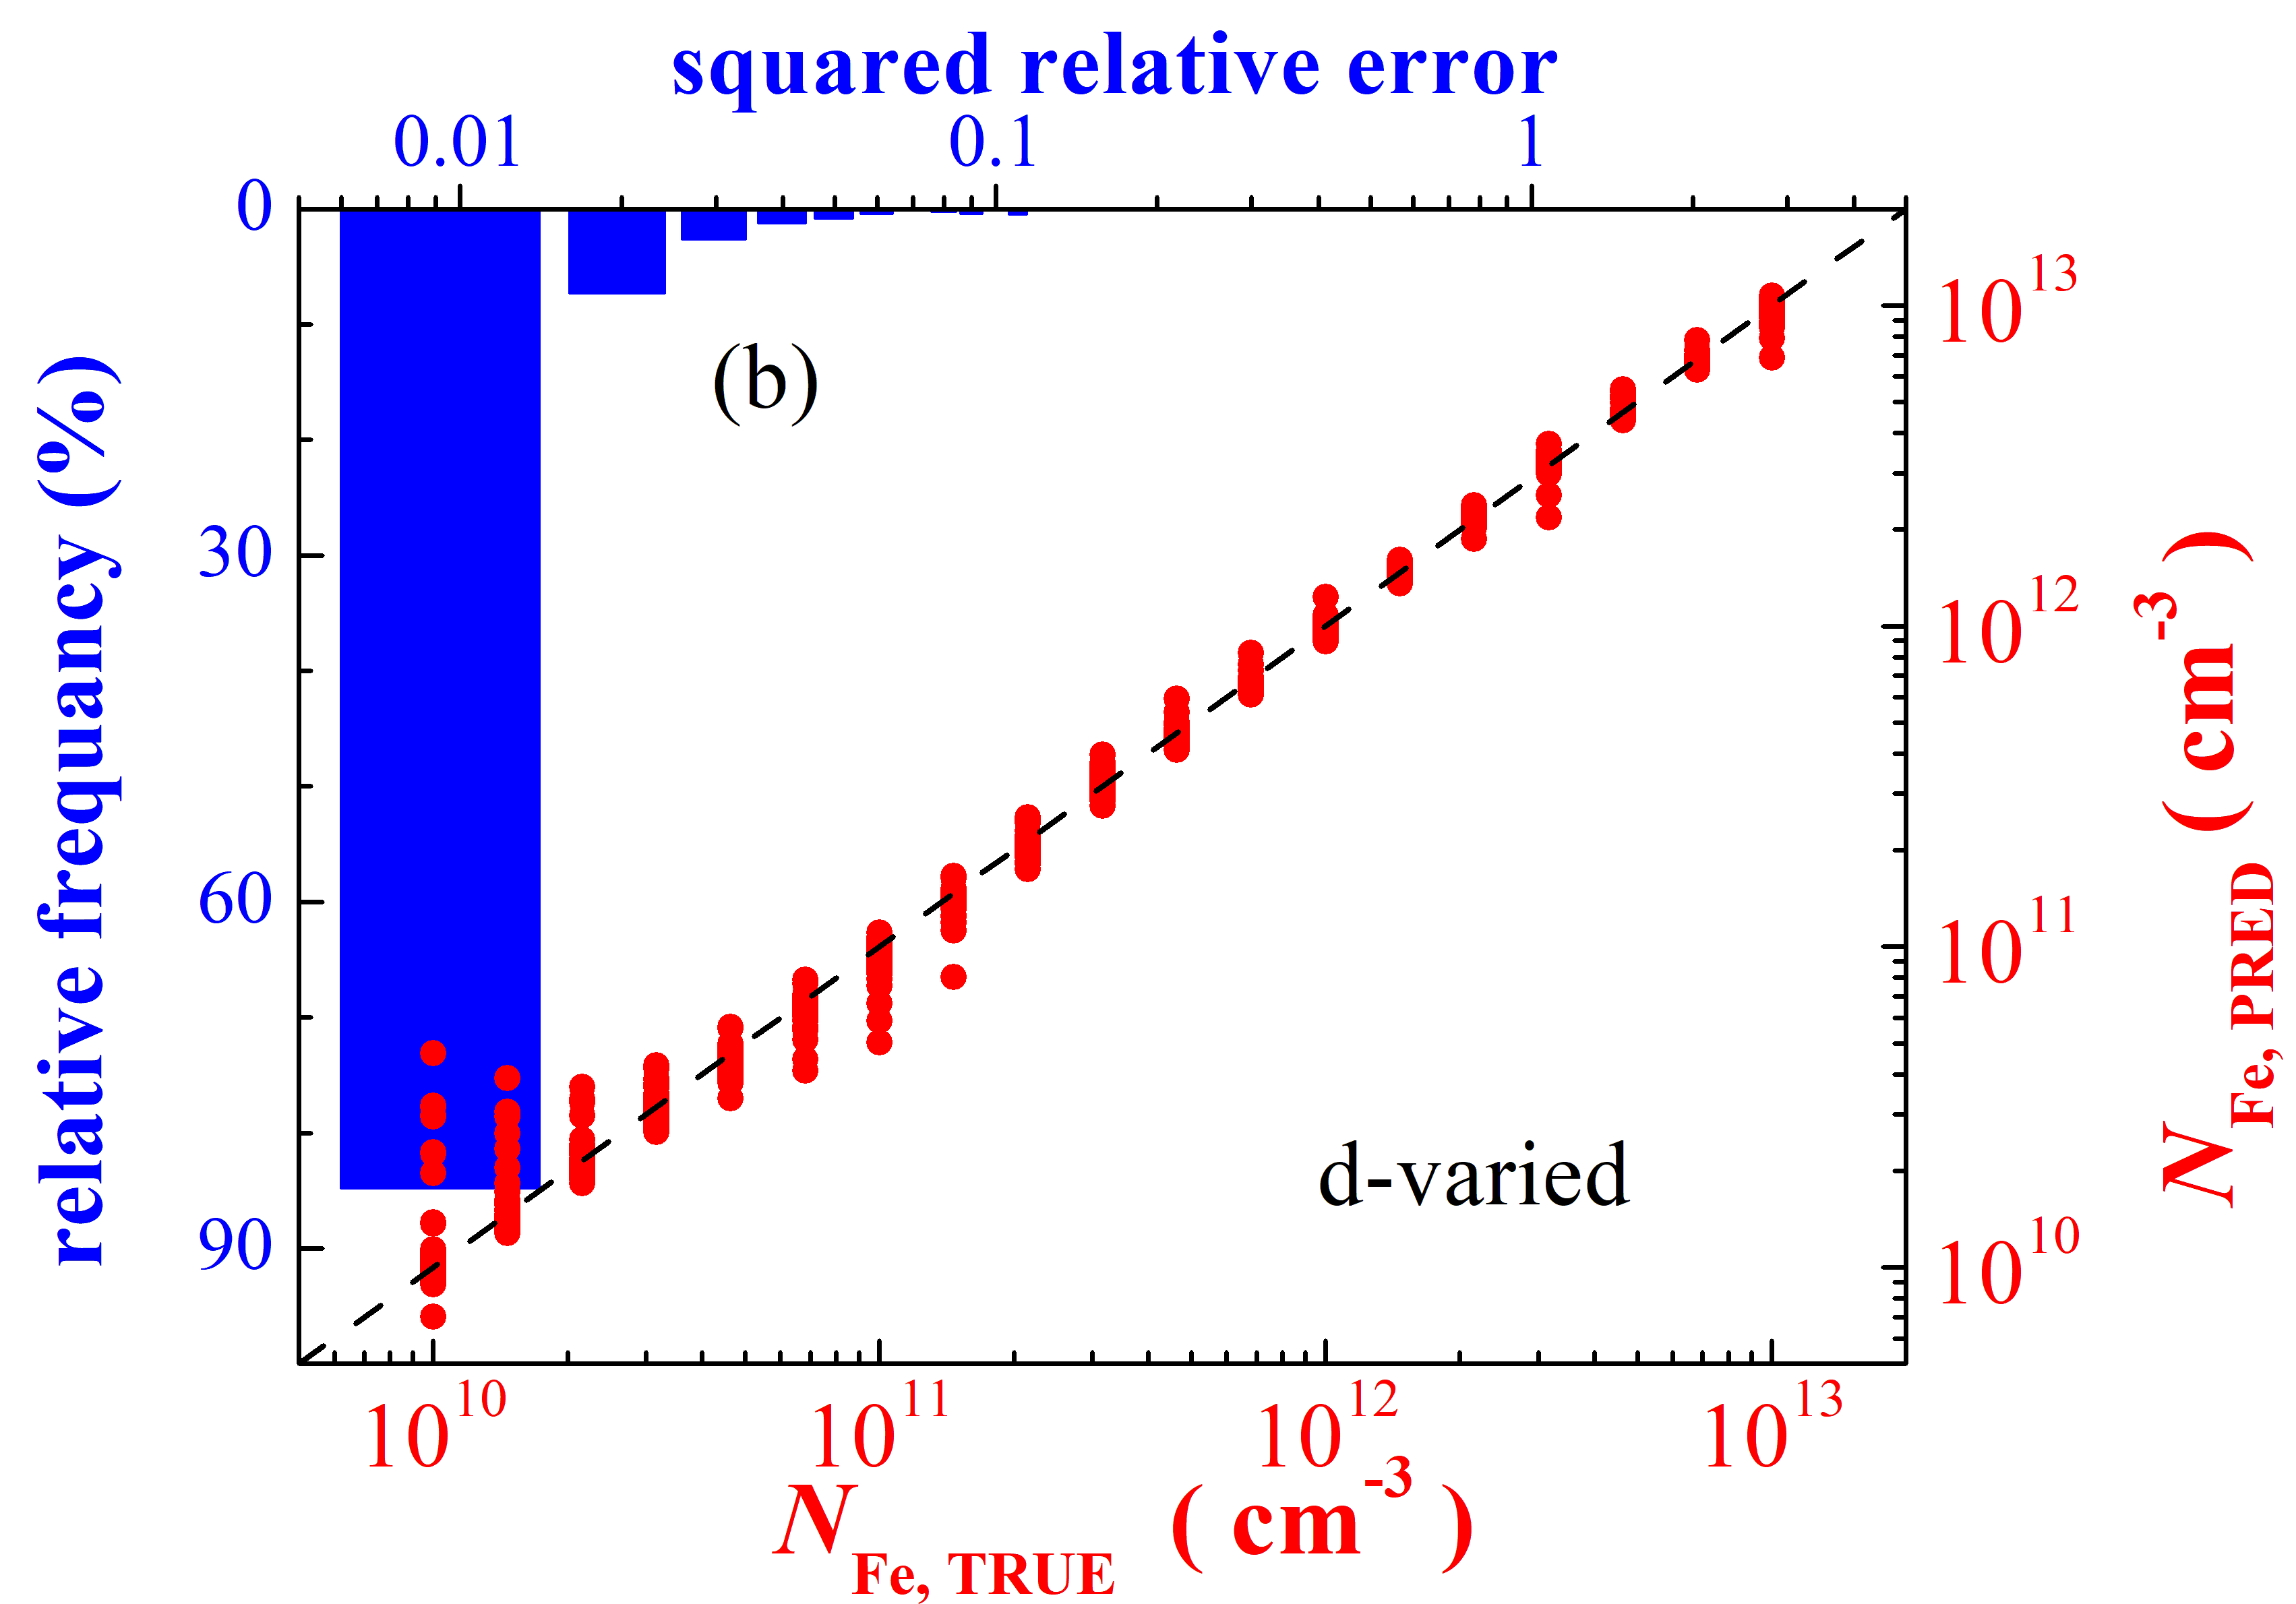
\includegraphics[width=0.32\textwidth]{F8b}
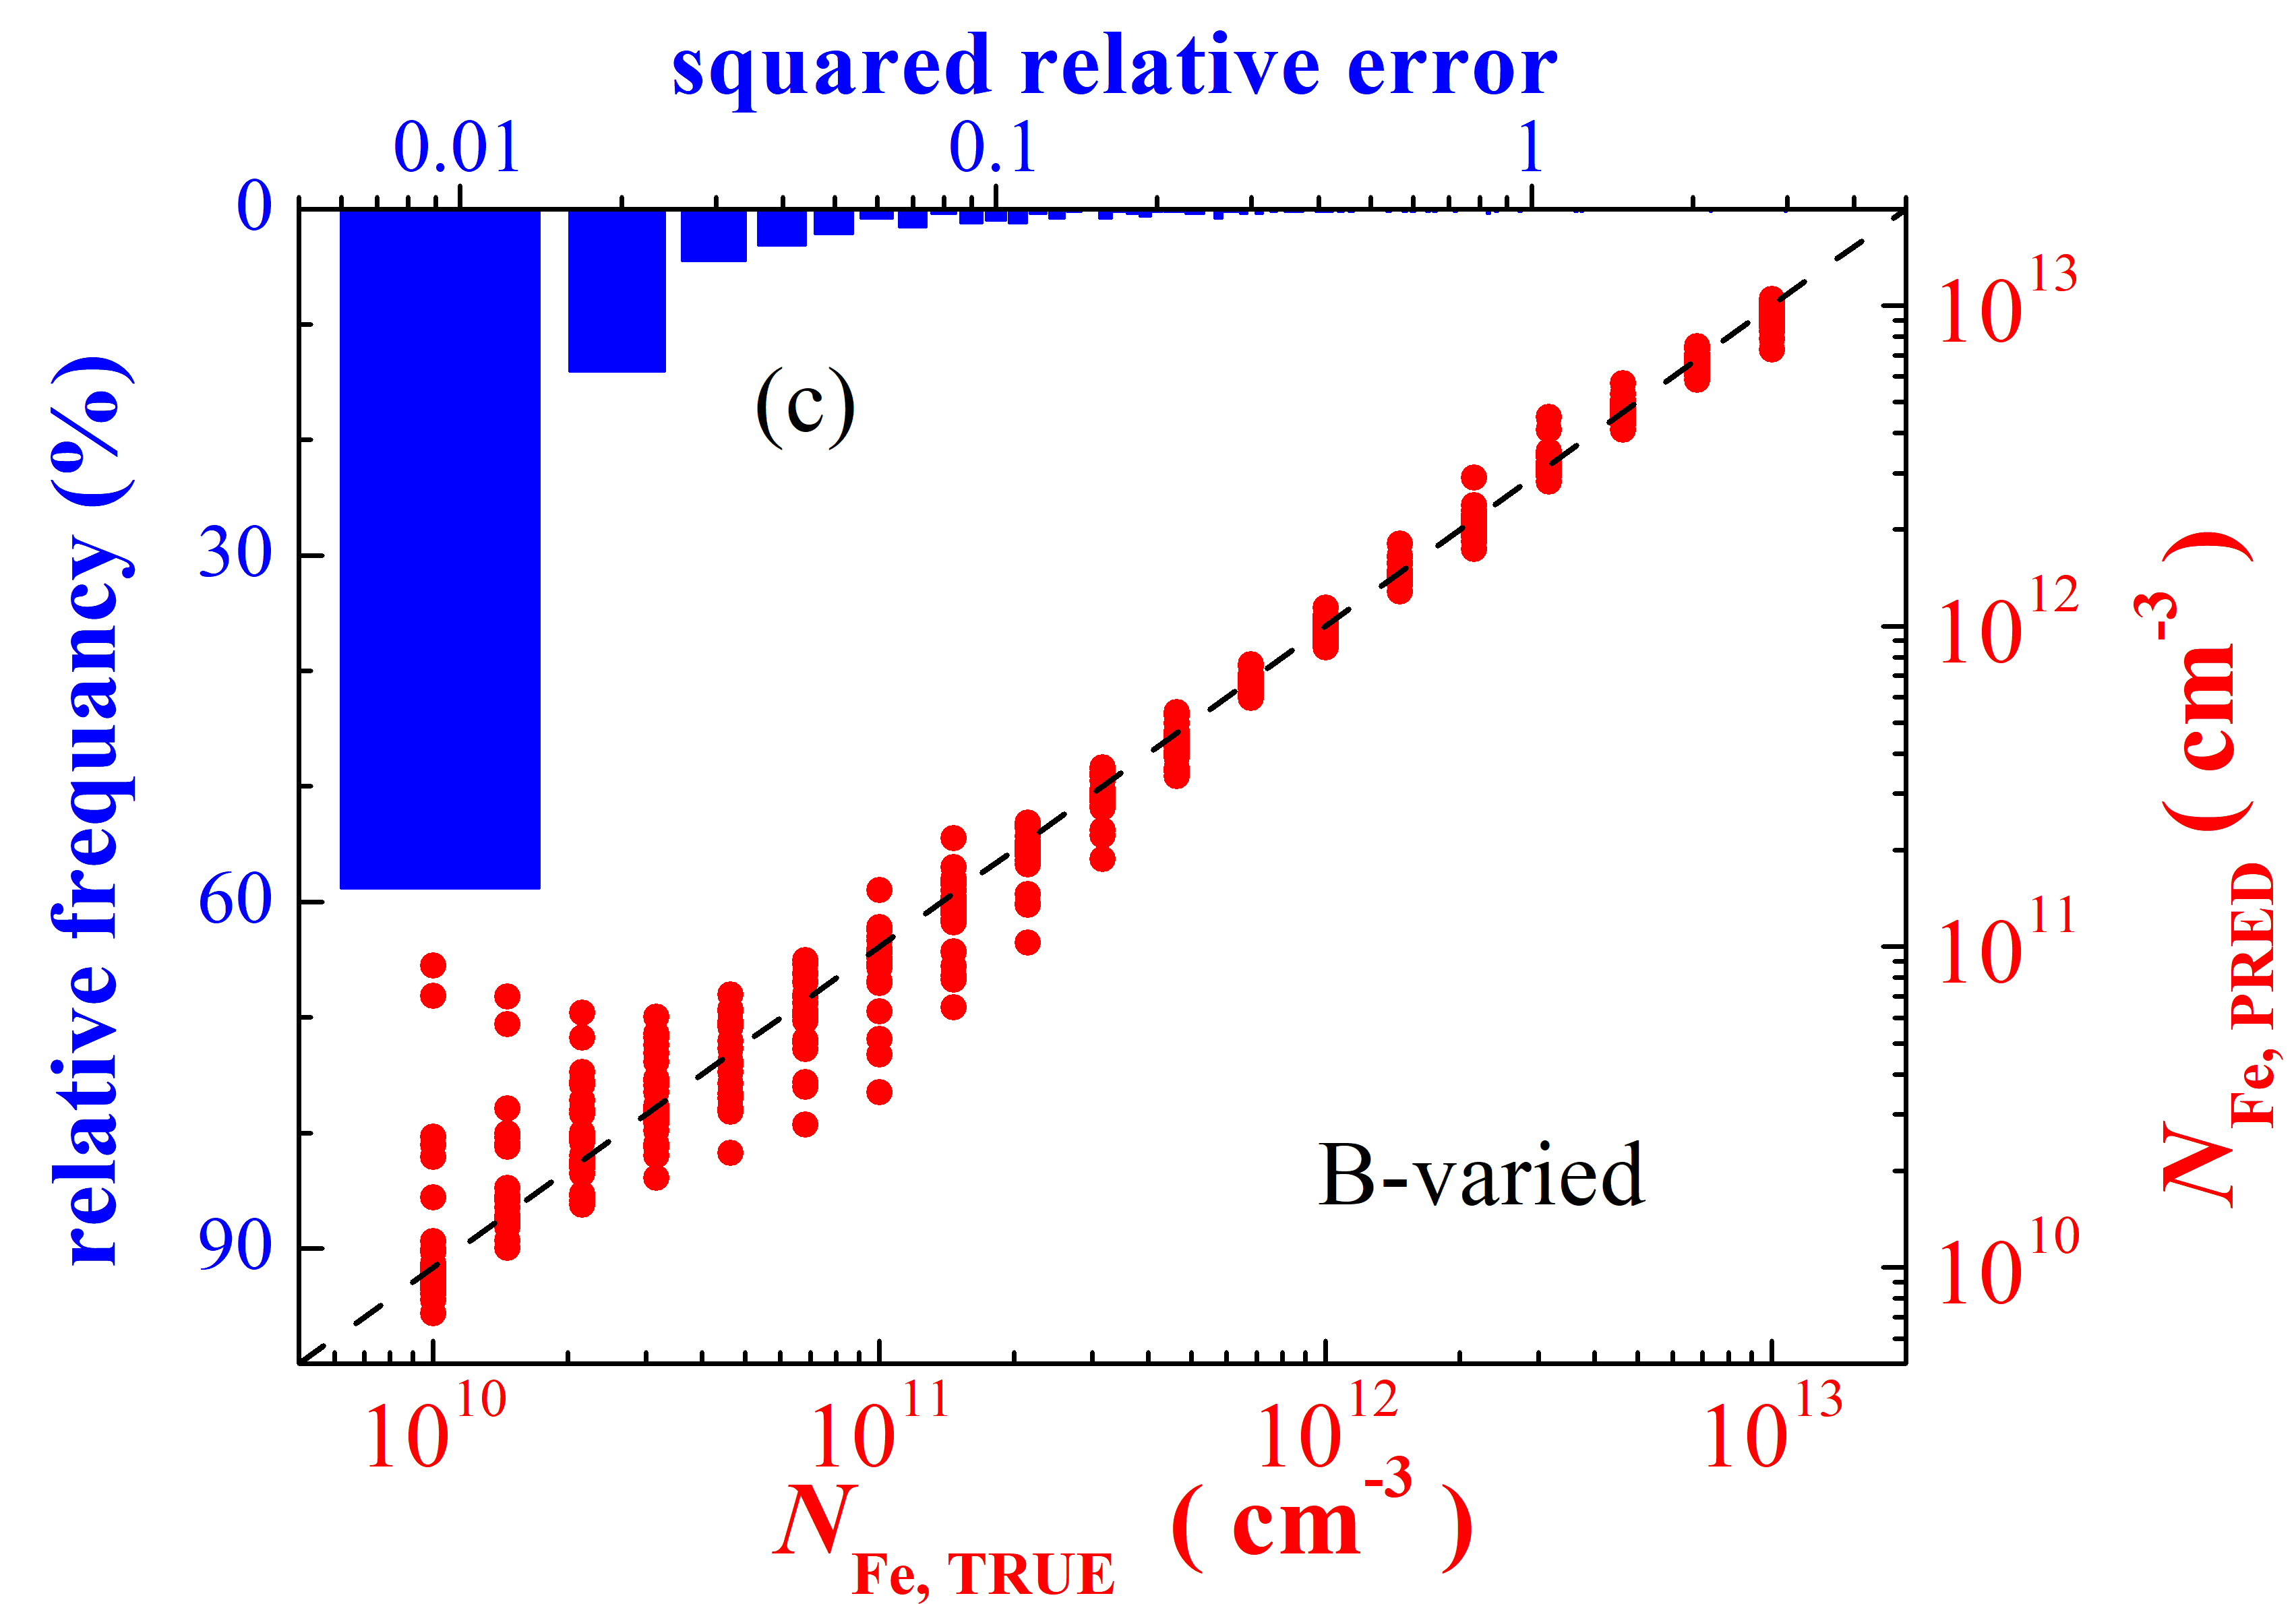
\includegraphics[width=0.32\textwidth]{F8c}
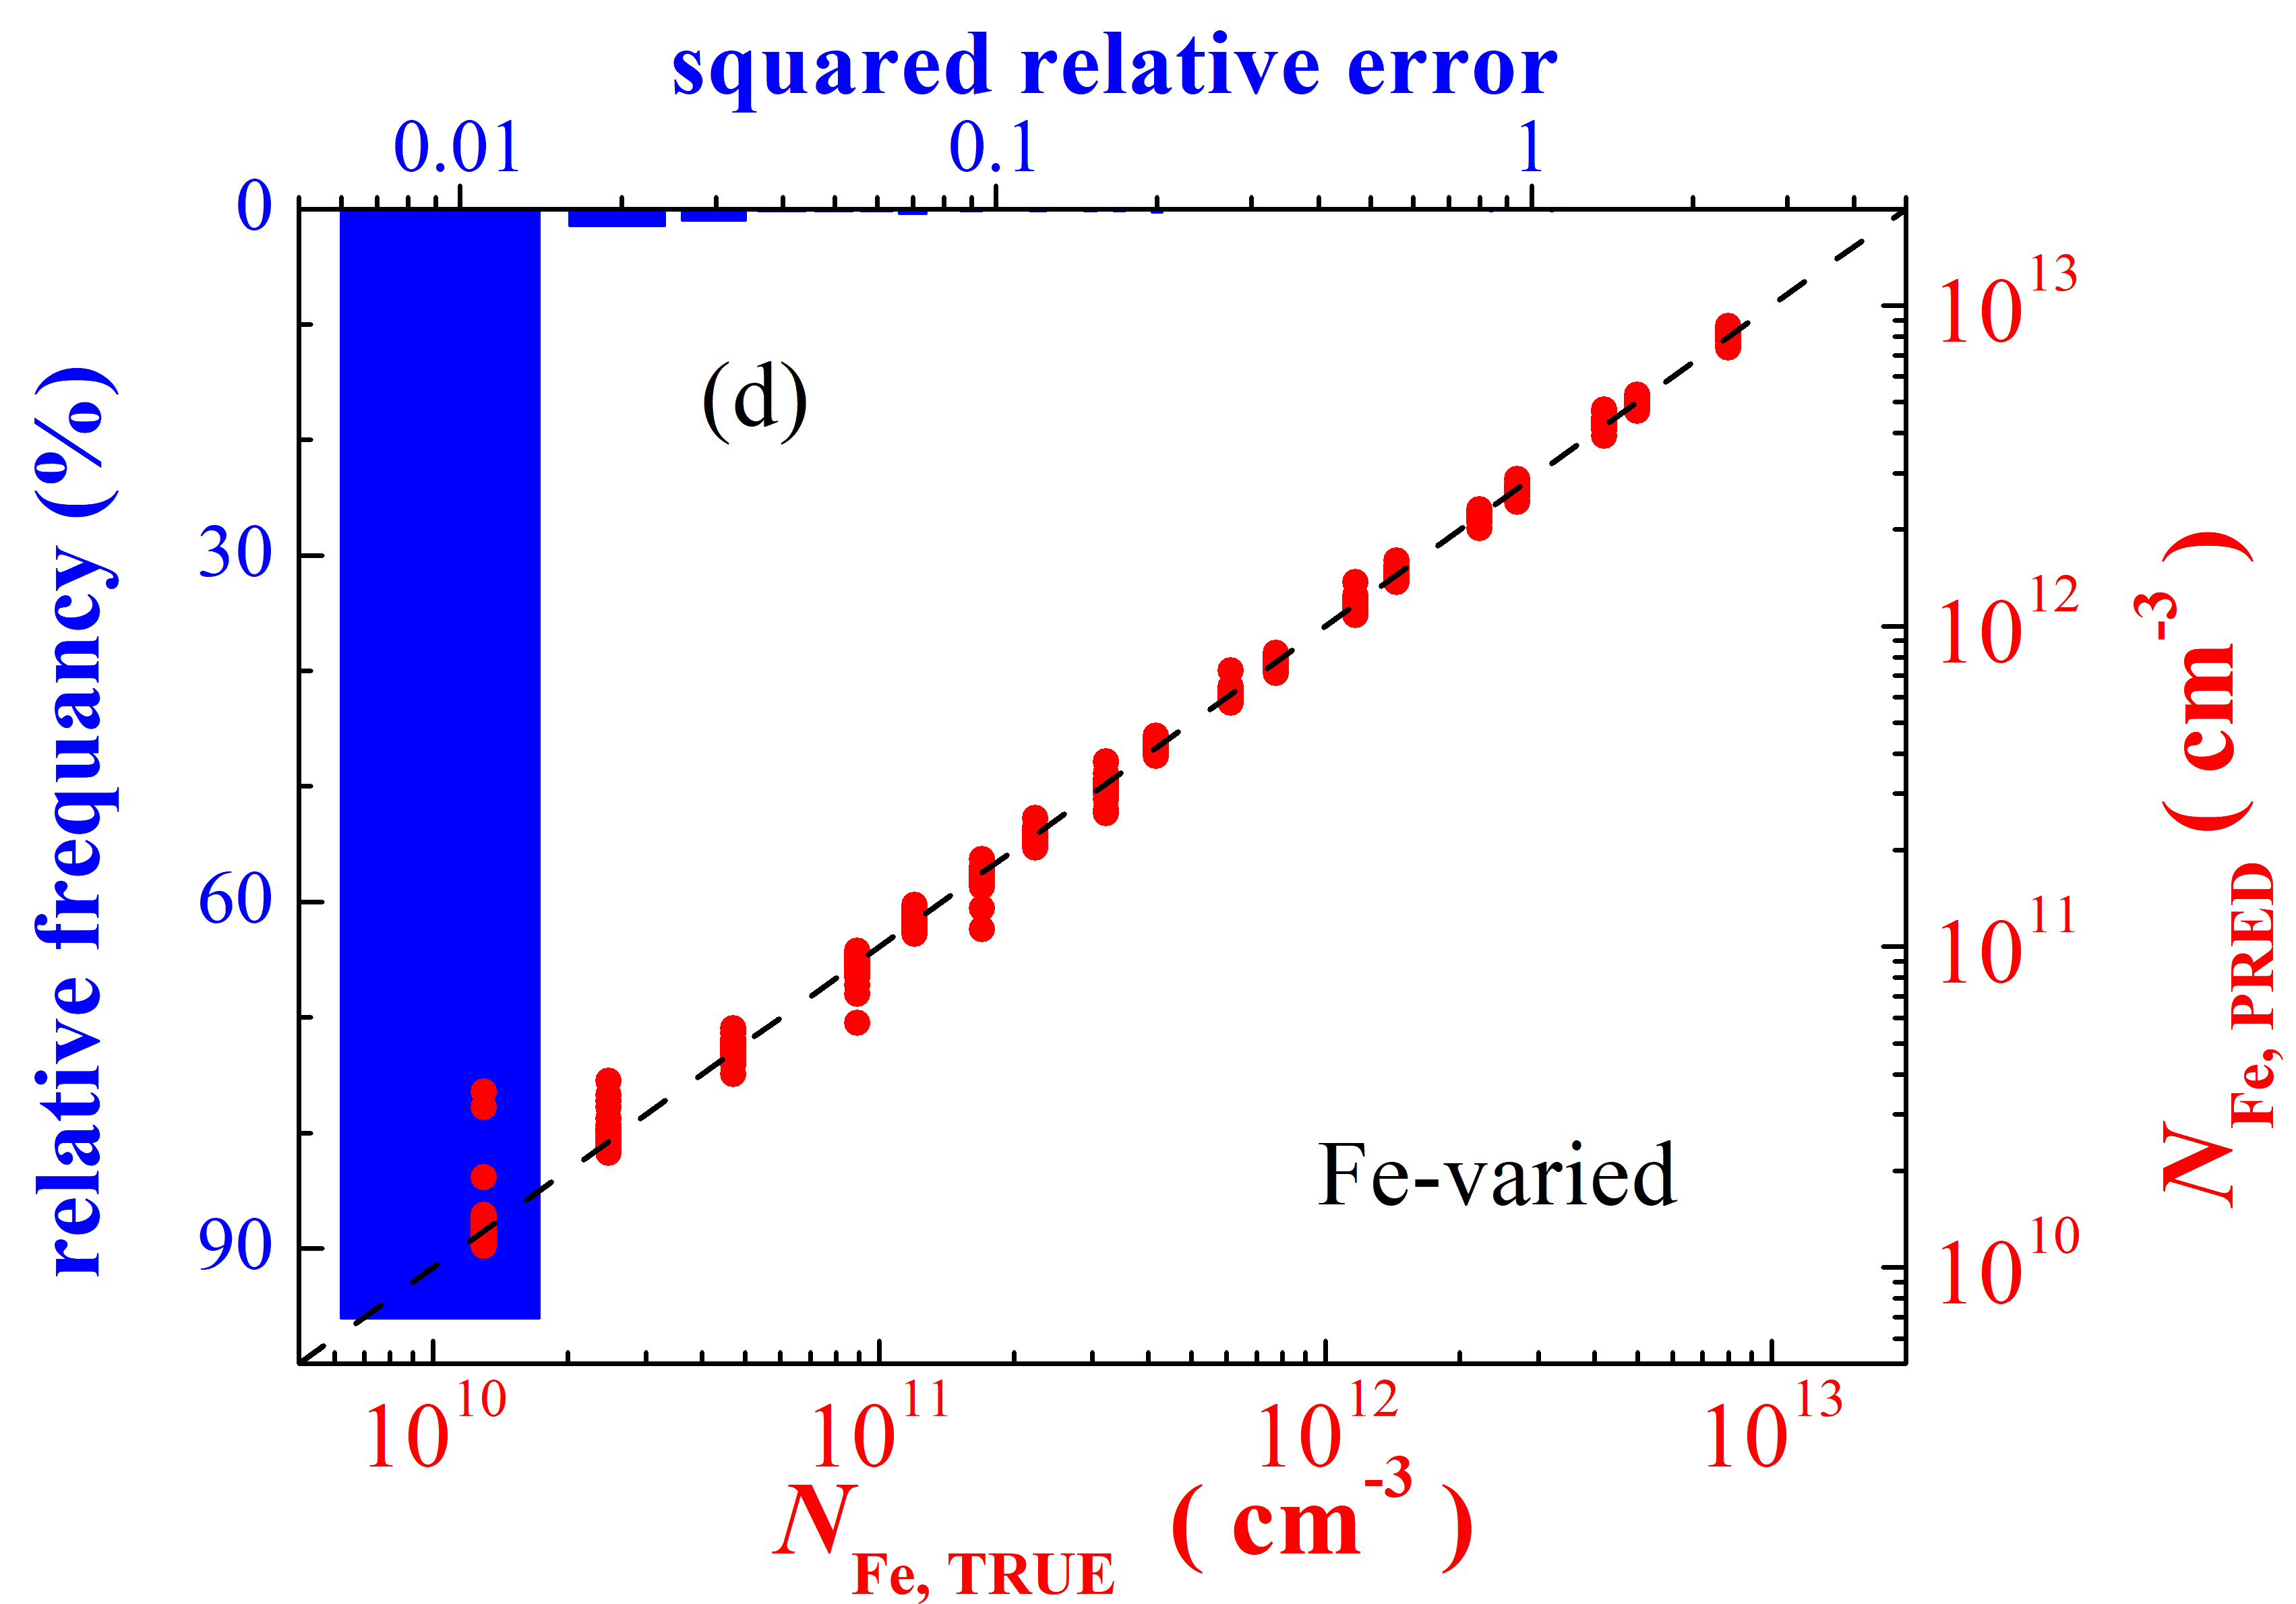
\includegraphics[width=0.32\textwidth]{F8d}
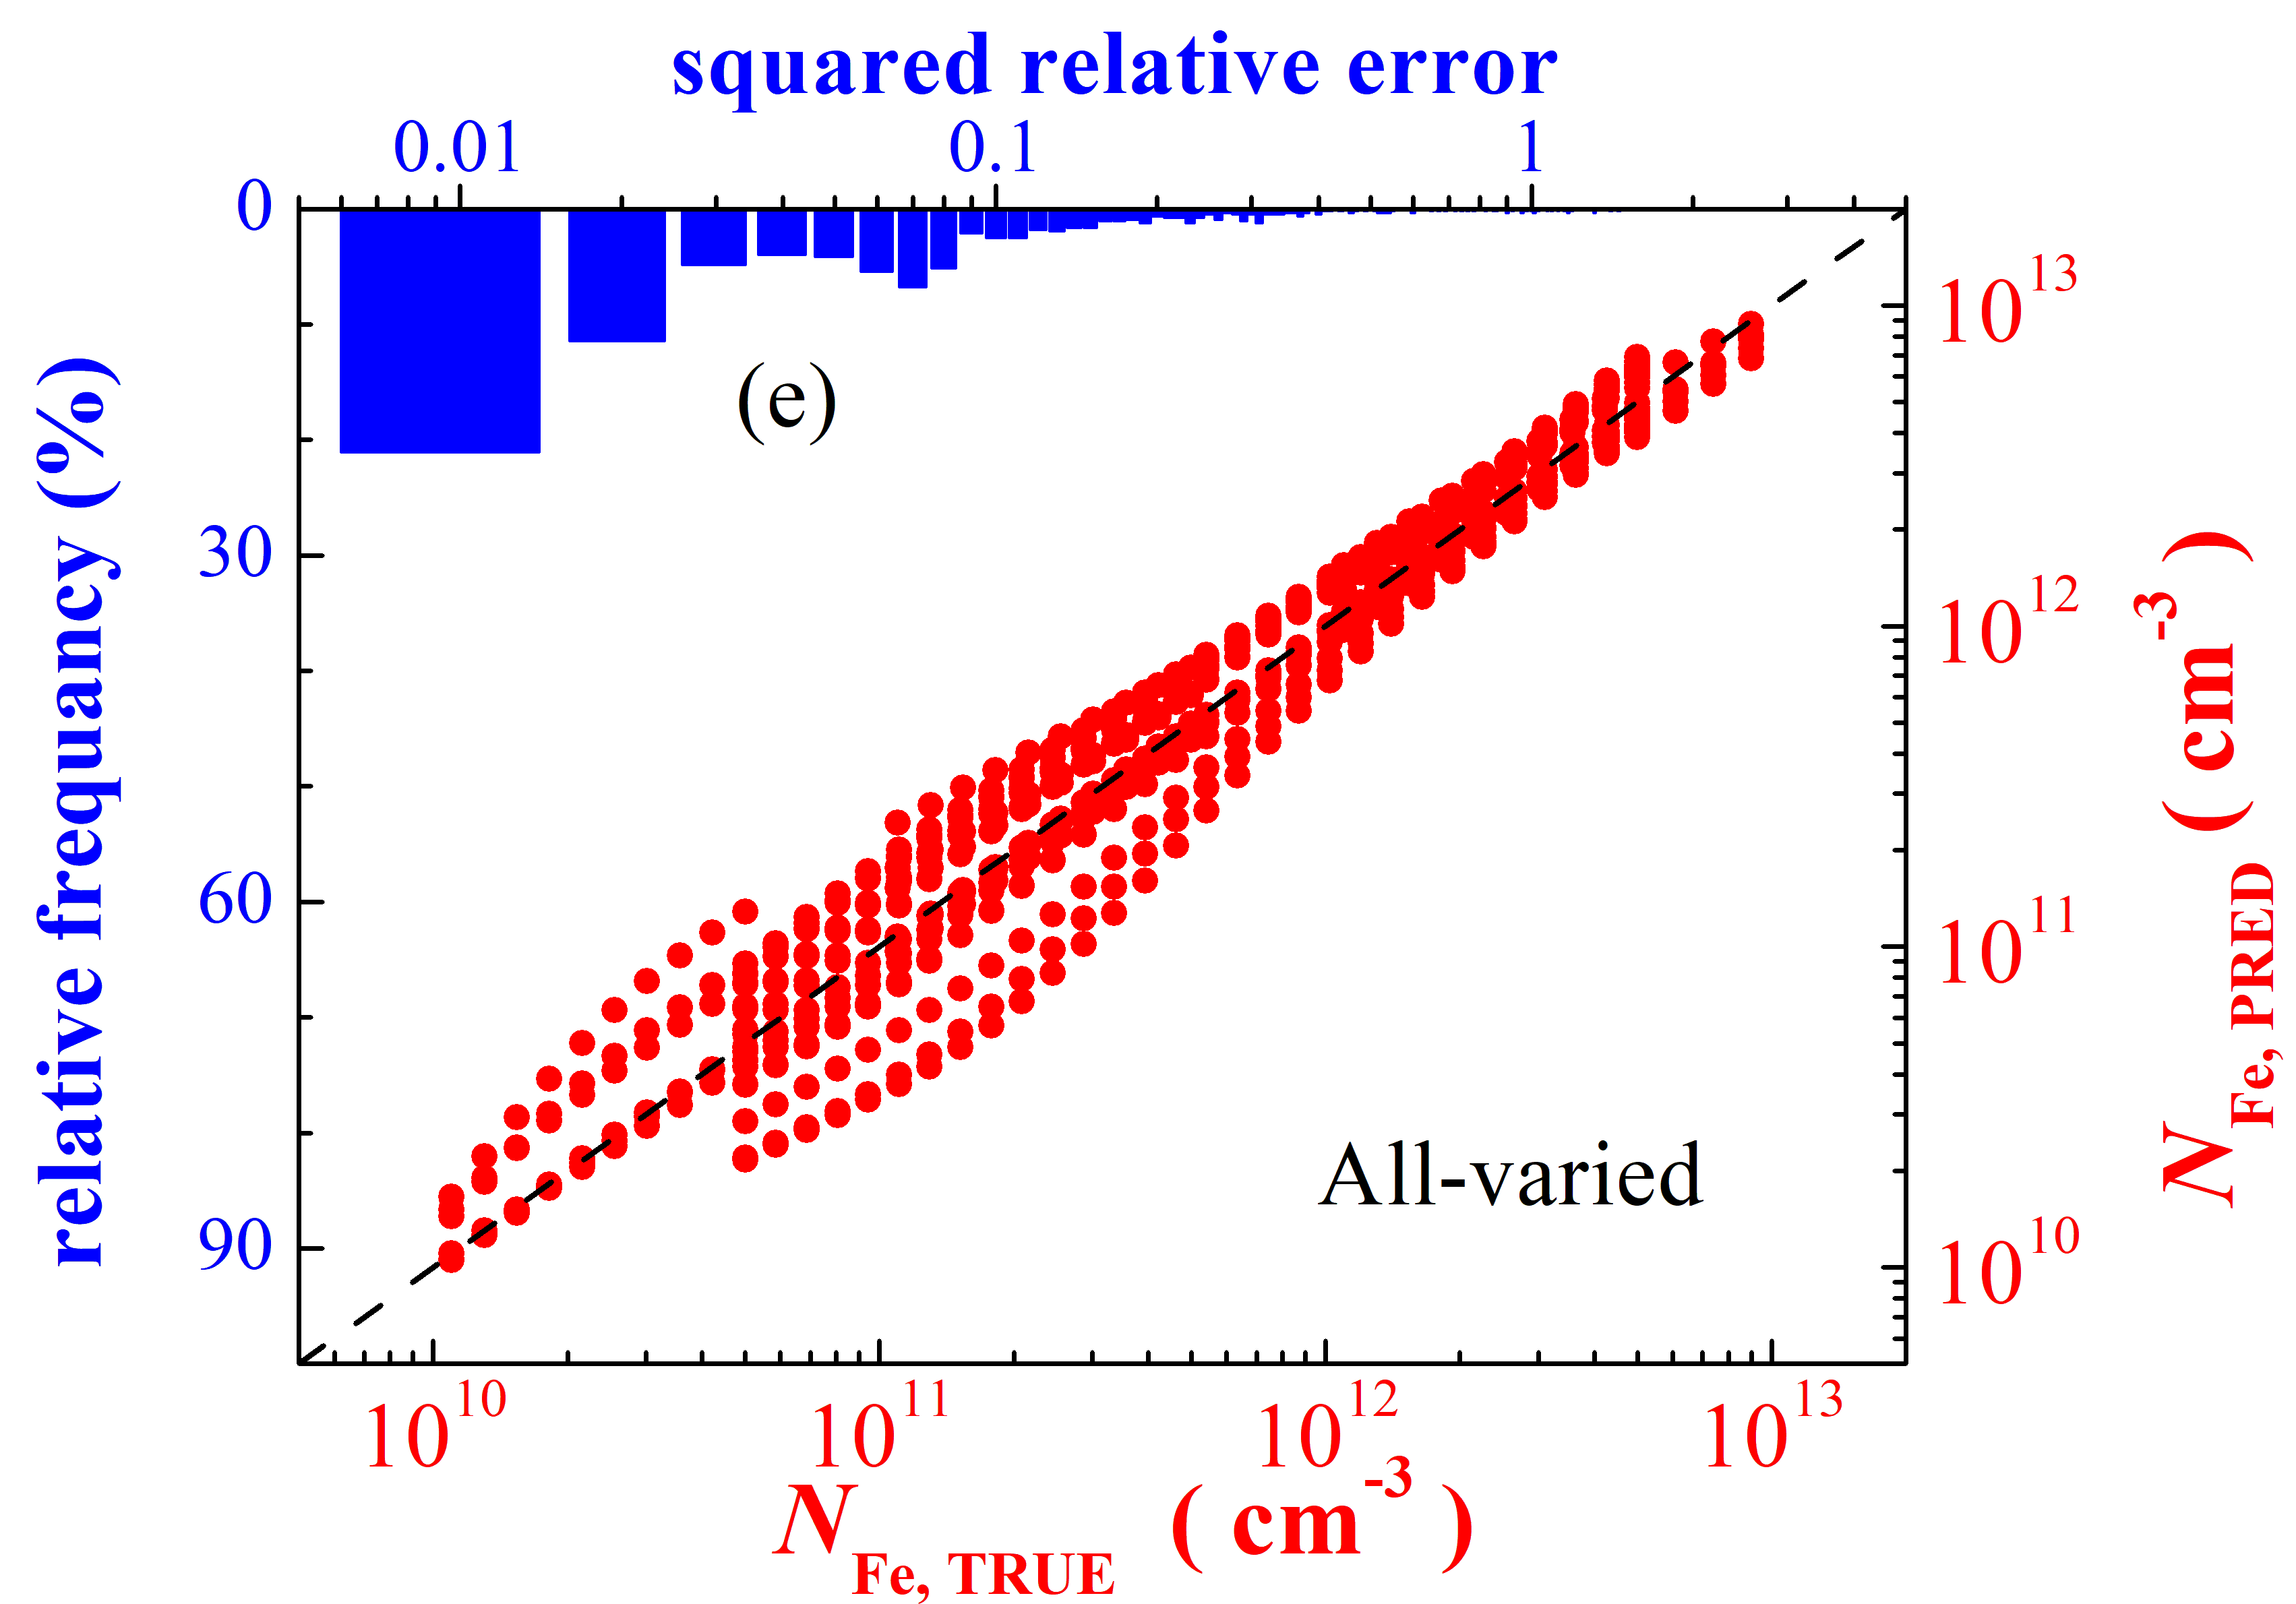
\includegraphics[width=0.32\textwidth]{F8e}
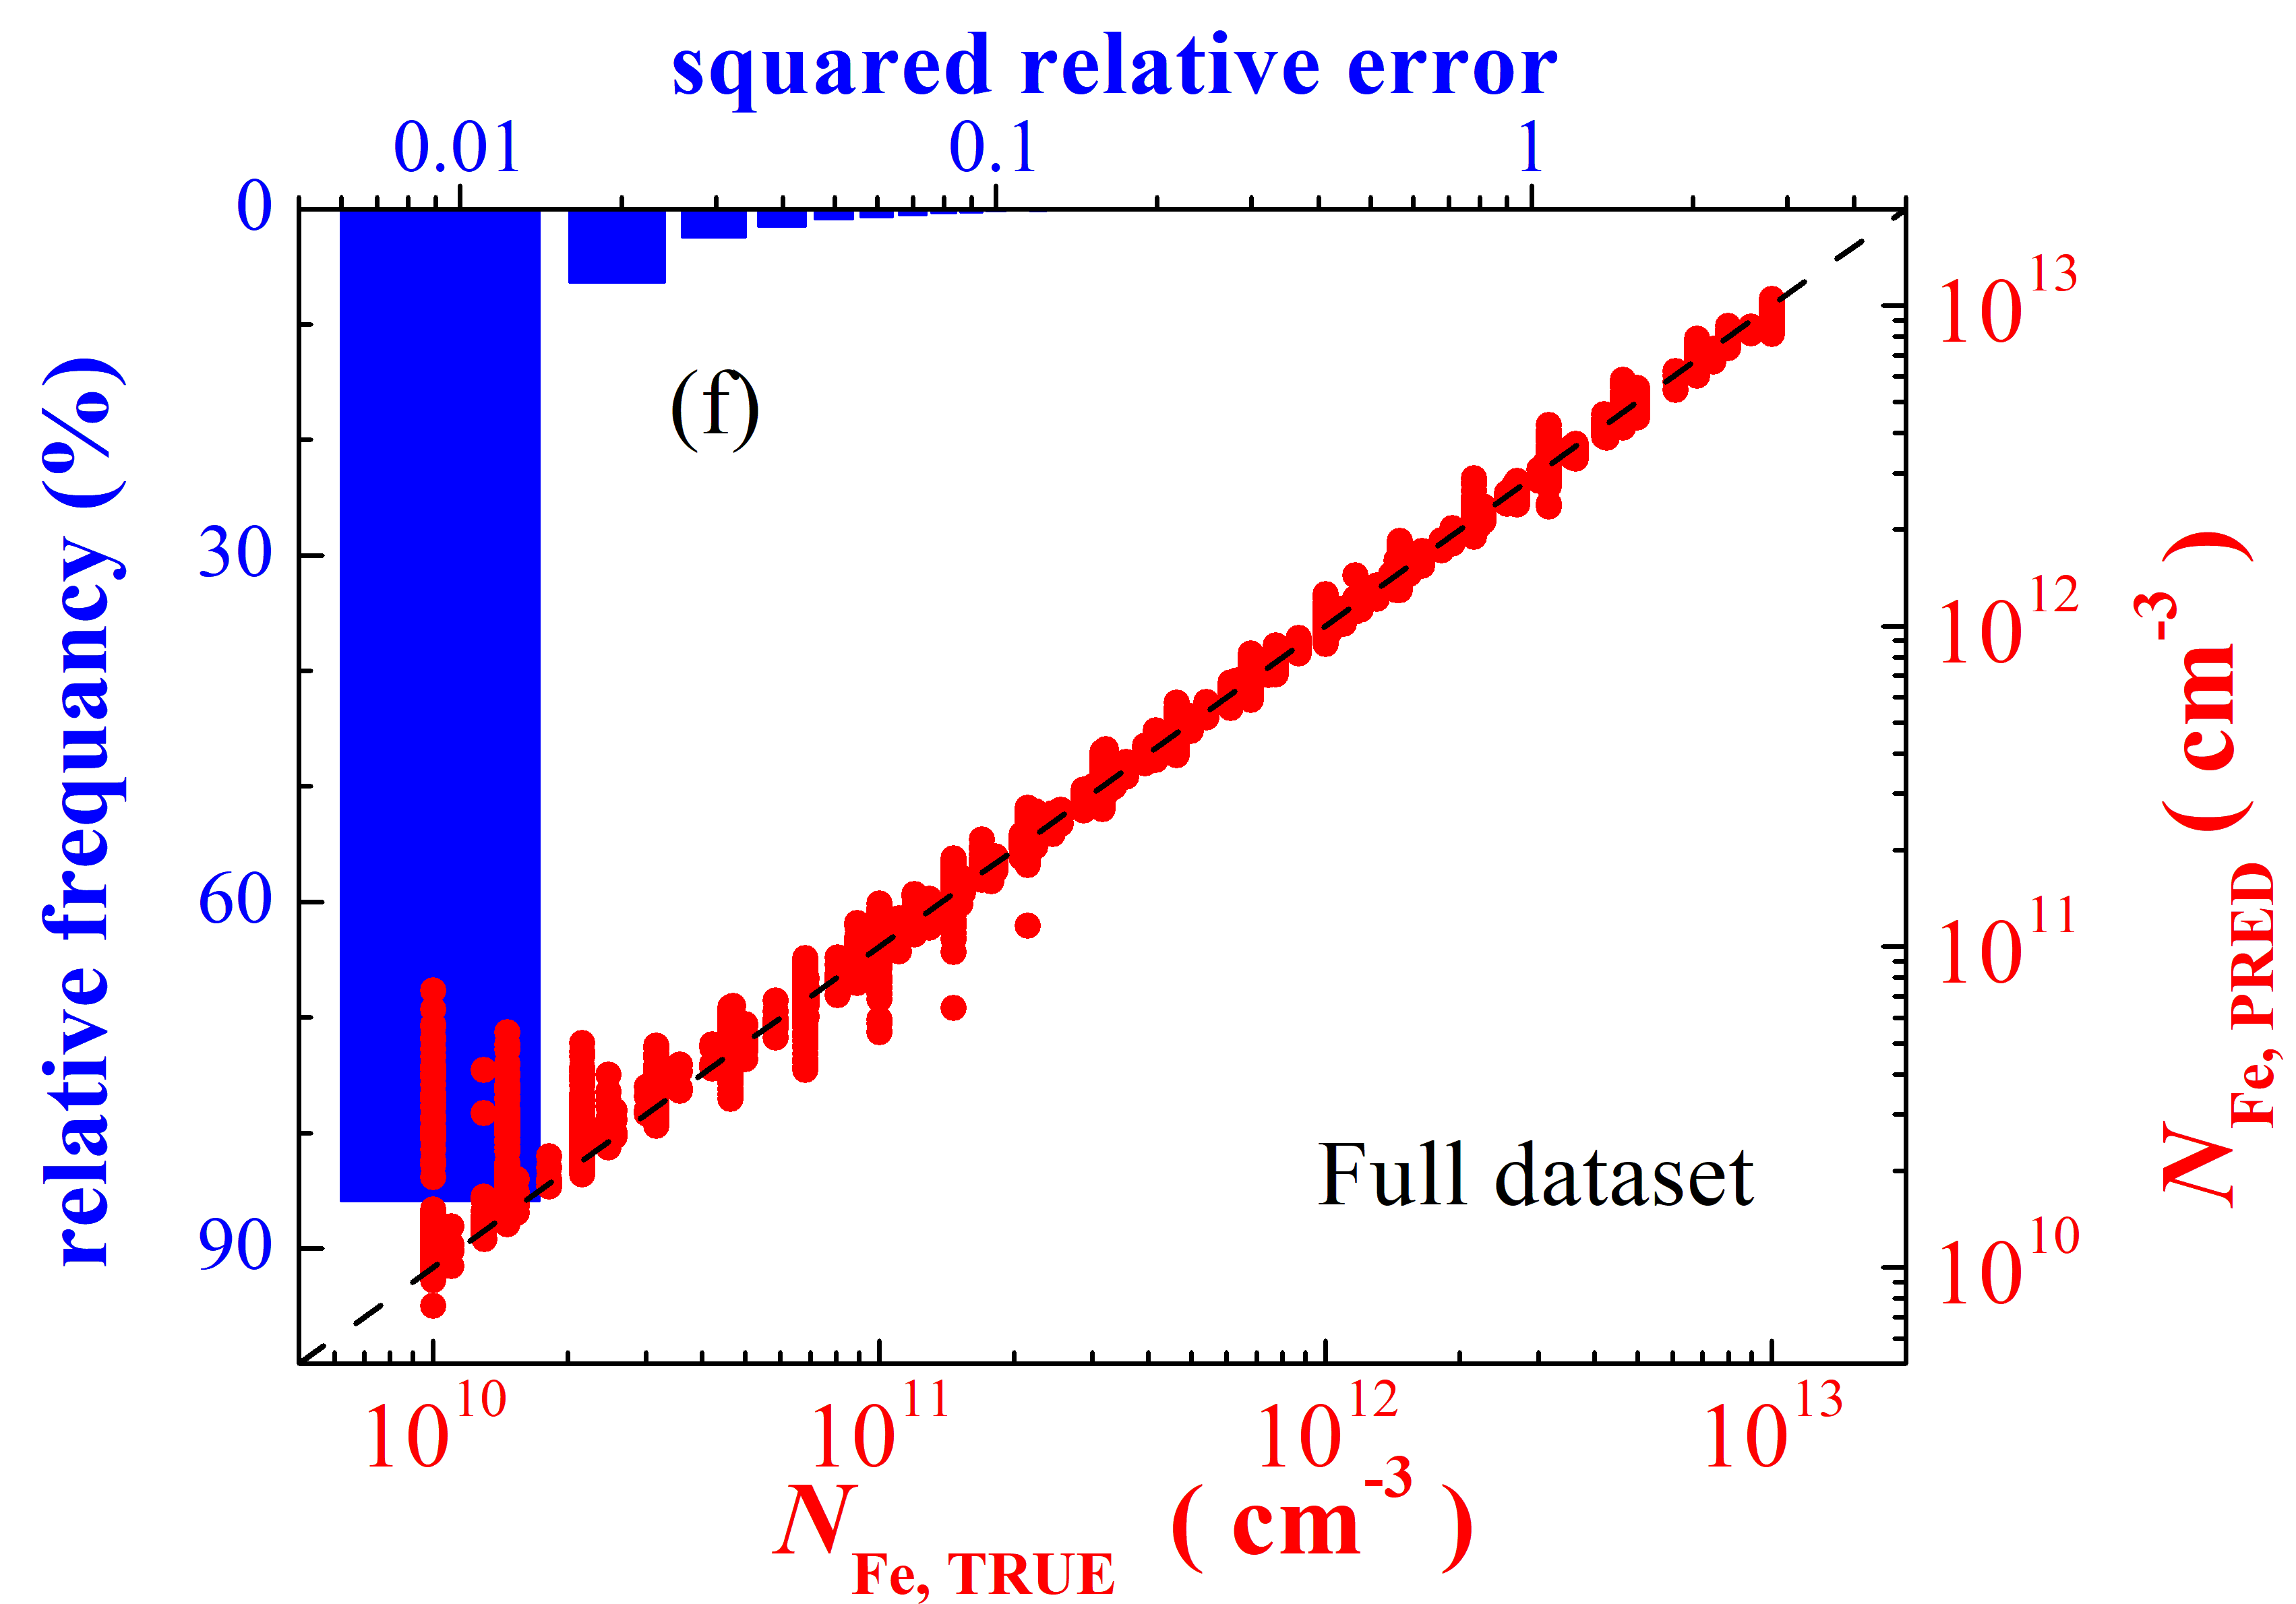
\includegraphics[width=0.32\textwidth]{F8f}
\caption{Iron concentrations are plotted against those generated by DNN$_\mathrm{FeFeB-Fe}$
on  T-varied (a),
d-varied (b),
B-varied (c),
Fe-varied (d),
All-varied (e),
and full (f) datasets (red points).
Bars represent histograms of squared relative error.
DNN was learned by training (a)--(e) or full (f) dataset.
The black dashed lines are the identify lines servings as the references.}
\label{fig_TrDNN2}
\end{figure}

Despite the difference in predicting accuracy,
DNN$_\mathrm{FeFeB-Fe}$ features are similar to DNN$_\mathrm{FeFeB}$ ones.
Thus
the DNN training with $N_\mathrm{B}$ values, which are expected in object of future research,
is important for prediction accuracy (Fig.~\ref{fig_TrDNN2});
the increase in the temperature value (Fig.~\ref{fig_Temp}) as well as decrease
in doping level (Fig.~\ref{fig_B}) or iron concentration (Fig.~\ref{fig_Fe})
results in error rise.
It should be noted that the prediction error gain with $N_\mathrm{Fe}$ increase not observed in DNN$_\mathrm{FeFeB-Fe}$ case and SRE range at $N_\mathrm{Fe}=10^{13}$~cm$^{-3}$ is more narrow then those at $N_\mathrm{Fe}=10^{10}$~cm$^{-3}$ --- see Fig.~\ref{fig_Fe}(b,c).

The results of training both DNN$_\mathrm{FeFeB}$ and DNN$_\mathrm{FeFeB-Fe}$ with full dataset
are presented in Table~\ref{table_CV}, Fig.~\ref{fig_TrDNN1}(f), and Fig.~\ref{fig_TrDNN2}(f).
One can see that the extension of the labeled dataset does not practically improve the DNN result in our case.
In our opinion, there is evidence of
i)~a good DNN configuration tuning;
ii)~a limited predictive ability of DNN$_\mathrm{FeFeB}$,
which caused by ambiguity of dependence $n_\mathrm{Fe-FeB}=f(N_\mathrm{Fe})$ .

\subsection{Experimental IV curves}

\cite{2021CMLTP,FeBAssJAP2014,FeBKin2019}

\begin{figure}[t]
\centering
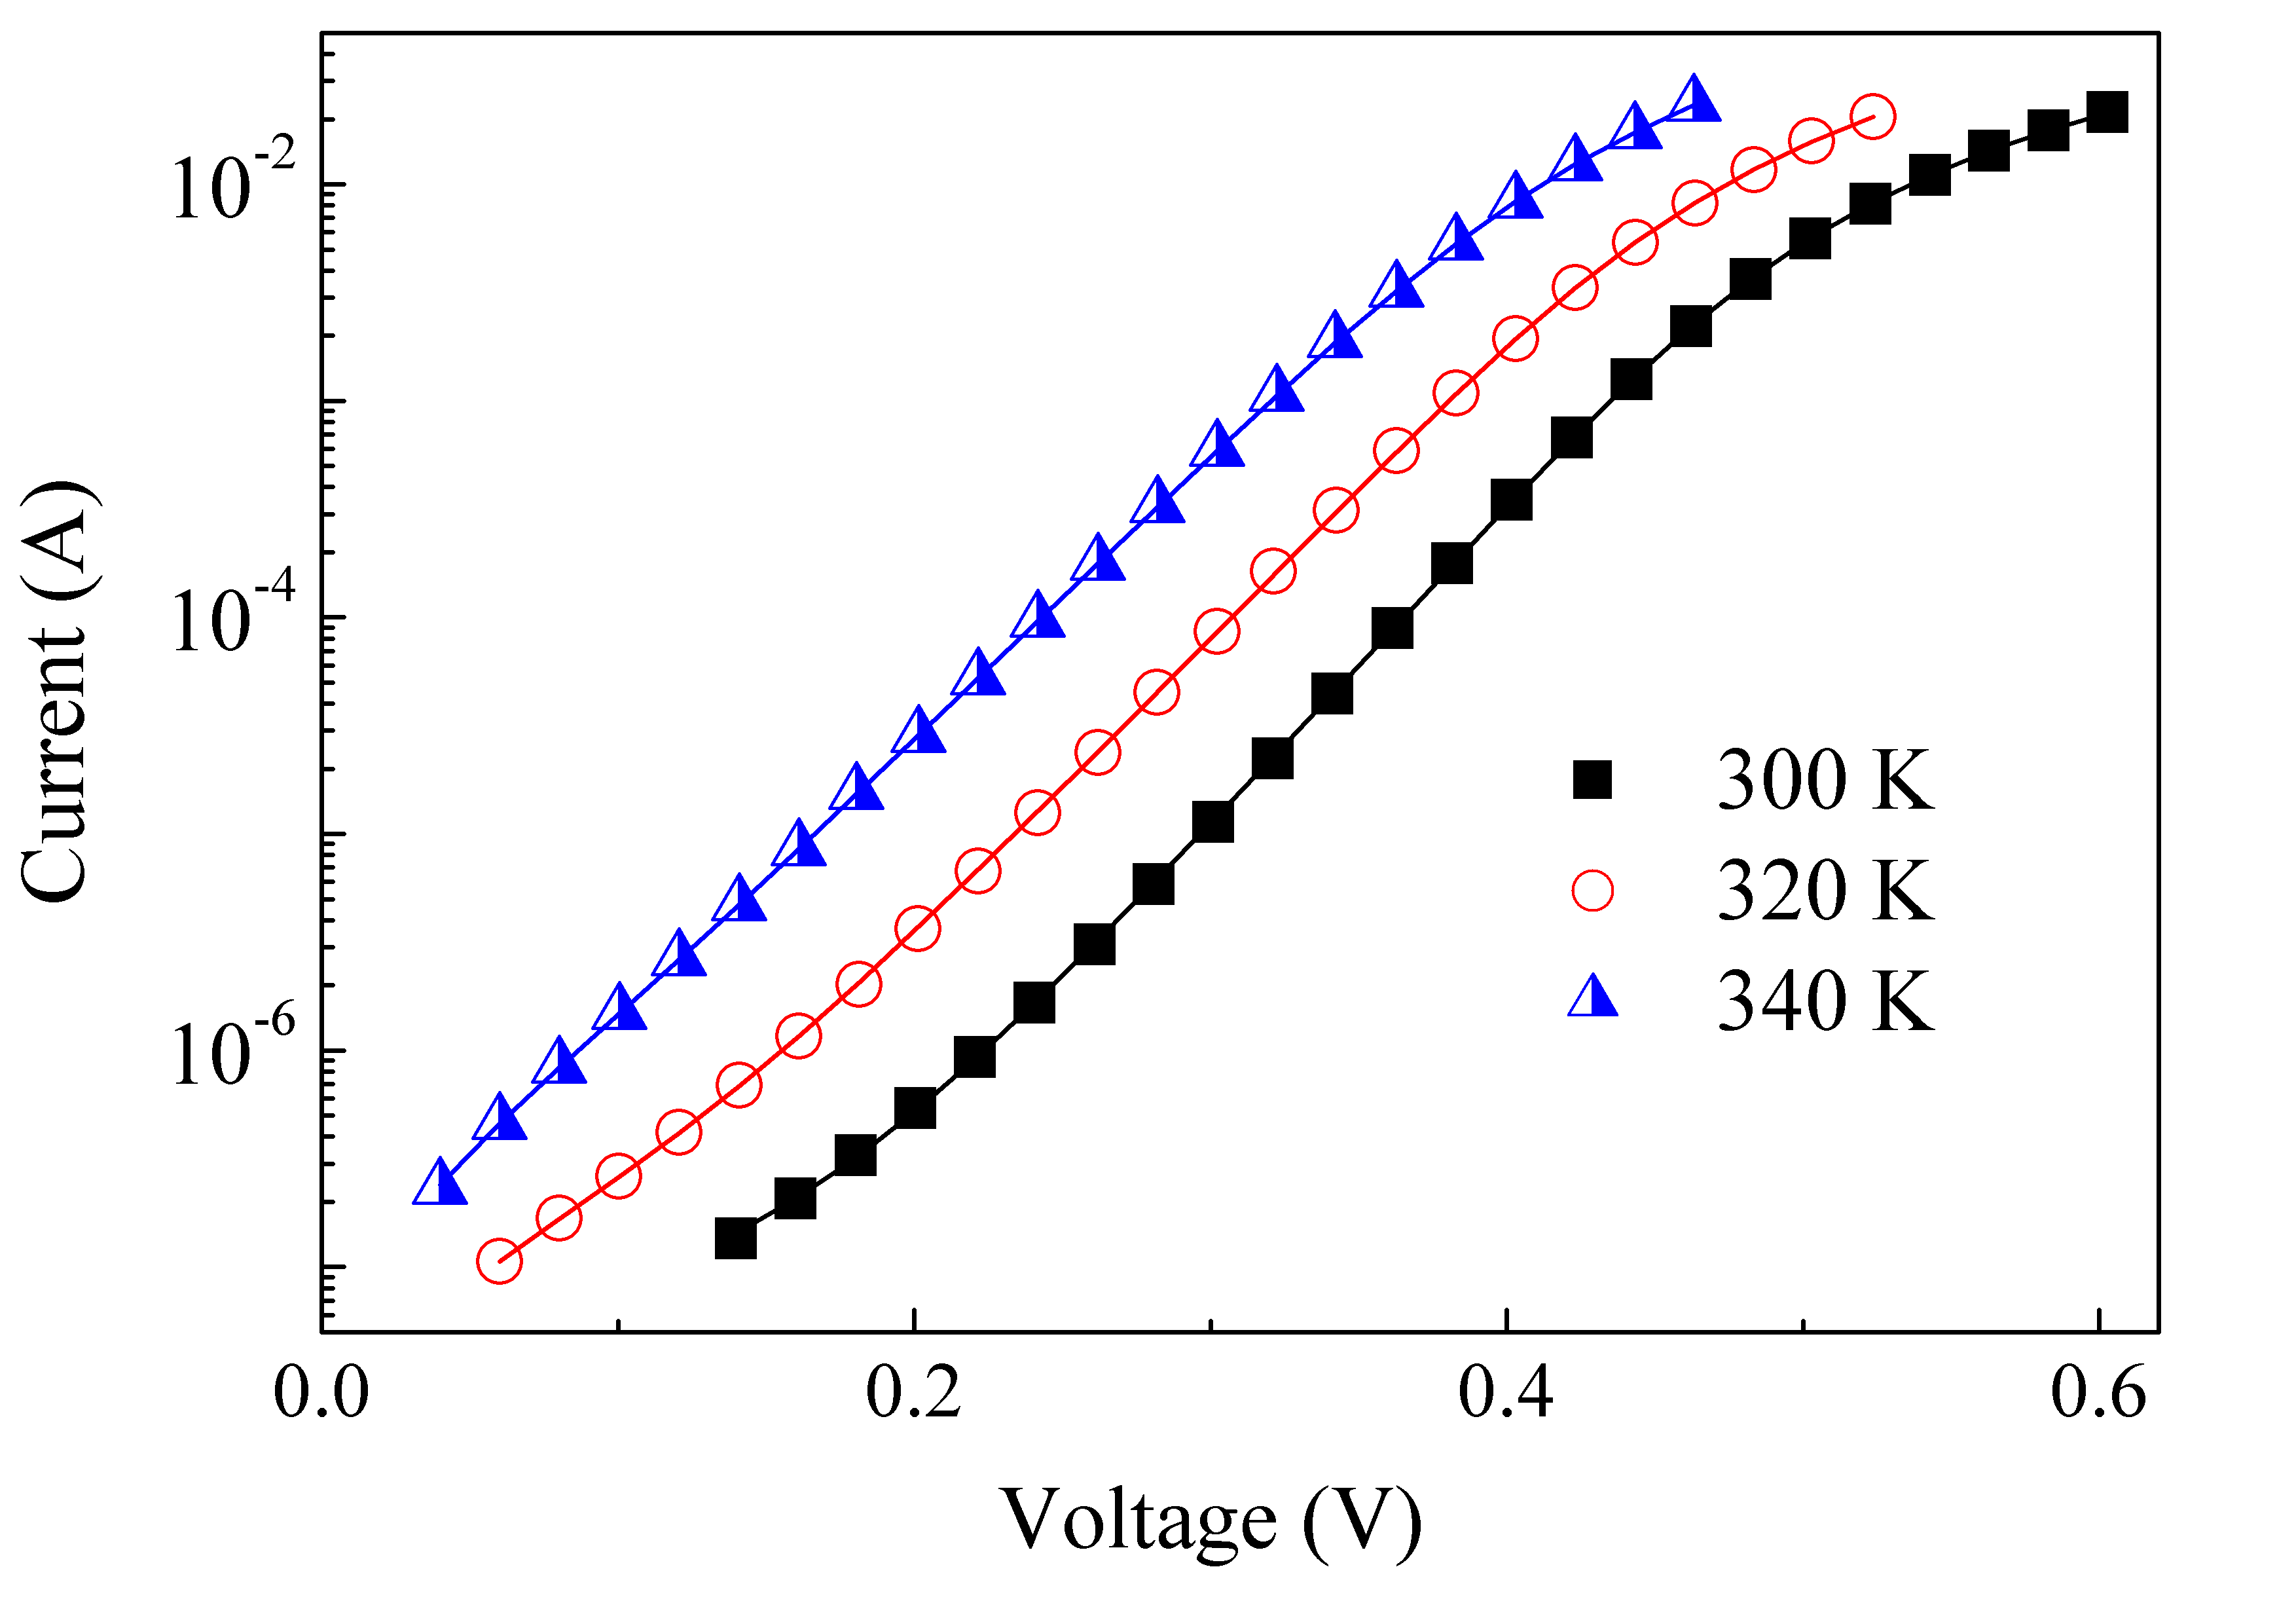
\includegraphics[width=0.5\textwidth]{F9}
\caption{
$I$–-$V$ characteristics measured at 300~K, 320~K, and 340~K for
sample SC320.
The marks are the experimental results, and
the solid lines are the curves fitted by
Eq.~(\ref{eqIVd}).
}
\label{fig_IVexp}
\end{figure}

\begin{table}
\caption{Results of experimental IV fitting and iron contamination testing}\label{table_Exp}
\begin{tabular}{lcccccccccc}%{\tblwidth}{@{} LLLLLLL@{} }
\headrow
\thead{Sample}&$N_\mathrm{Fe,MEAS}$, &$T$,&
$n_\mathrm{Fe-FeB}$&$R_{sh,\mathrm{Fe-FeB}}$,&
$n_\mathrm{Fe}$&$R_{sh,\mathrm{Fe}}$,&
\multicolumn{4}{c}{$N_\mathrm{Fe,PRED}$, $10^{12}$~cm$^{-3}$}\\
\headrow
&$10^{12}$~cm$^{-3}$&K&&Ohm&&Ohm&\multicolumn{2}{c}{DNN$_\mathrm{FeFeB}$}&\multicolumn{2}{c}{DNN$_\mathrm{FeFeB-Fe}$}\\
\headrow
&&&&&&&training&full&training&full\\
\#320&$2.0\pm0.4$&300&1.214&$1.6\cdot10^6$&1.195&$1.4\cdot10^6$&3.9&2.8&3.0&2.0\\
&&320&1.204&$8.6\cdot10^5$&1.148&$8.0\cdot10^5$&6.6&1.9&16&19\\
&&340&1.118&$4.3\cdot10^5$&1.111&$4.3\cdot10^5$&3.8&1.2&89&574\\
\#349&$6.7\pm0.7$&300&1.223&$2.9\cdot10^6$&1.222&$2.6\cdot10^6$&8.9&5.6&15&11\\
&&320&1.183&$1.7\cdot10^6$&1.182&$1.7\cdot10^6$&1.2&0.4&10&32\\
&&340&1.138&$1.3\cdot10^6$&1.173&$1.3\cdot10^6$&9.8&1.7&26&411\\
\hline
\end{tabular}
\end{table}

%N_\mathrm{Fe,PRED}

\section{Conclusion and Outlook}
In this paper,
we extracted the iron concentration in silicon BSF solar cells from an
ideality factor value and systematically studied the performance
of deep learning in this problem.
This work  is the first attempt at using deep learning for deep levels parameter retrieval from the current--voltage curve.
In this model study, we used simulation to obtain training and test labeled datasets.
Besides, a DNN was trial-tested by using the parameters of actual solar cells.
Our results showed the ability of the deep neural network
to predict iron concentration by using ideality factor values,
SC base thickness and doping level, and temperature.
MSRE was up to 0.005 for synthetic datasets.
The simulation has shown the prospects for the use of two ideality factor values  (for structure with $\mathrm{Fe}_i$ only as well as with $\mathrm{Fe}_i\mathrm{B}_s$ and $\mathrm{Fe}_i$ coexistence)
for upgrading  a prediction accuracy.
At the same time, the practical application of such an approach manifested difficulties in obtaining correct data.
It was important to train DNN with a boron concentration value,
which agreed with the doping level of investigated structures.
Moreover, the increase in iron concentration or boron concentration, as well as temperature decrease,
results in a prediction error reduction.

The proposed approach envisages
the utilization of a simple and widely applicable setup and
does not require much time.
Therefore it could be integrated into a manufacturing environment.
However, it should be noted that we have simplified the task for our purposes.
In our opinion, there are two ways of further improve the method.
The first one connects with the refining of labeled datasets and can be realized by
using 3D-simulators (e.g., SILVACO TCAD) or real IV measurements in a broad set of SCs.
The improvement of DNN operation is the second one;
and the fine-tuning is like most promising in this case.
For example,
not numerous input parameters can be multiplied and transformed to the picture and
apply a vision model (e.g., VGG16).



\section*{Acknowledgments}
This work was supported by National Research Foundation  of Ukraine
(project number 2020.02/0036)

\section*{Conflict of Interest}
The authors declare that they have no known competing financial interests or
personal relationships that could have appeared to influence the work reported
in this paper.
%You may be asked to provide a conflict of interest statement during the submission process. Please check the journal's author guidelines for details on what to include in this section. Please ensure you liaise with all co-authors to confirm agreement with the final statement.

\section*{Data availability}

The simulated IV characteristics, $n_\mathrm{Fe}$ and $n_\mathrm{Fe-FeB}$ values,
and trained DNNs are available
at \newline
\emph{https://github.com/olegolikh/IVcharacteristics.git}.

%\section*{Supporting Information}
%Supporting information is information that is not essential to the article, but provides greater depth and background. It is hosted online and appears without editing or typesetting. It may include tables, figures, videos, datasets, etc. More information can be found in the journal's author guidelines or at \url{http://www.wileyauthors.com/suppinfoFAQs}. Note: if data, scripts, or other artefacts used to generate the analyses presented in the paper are available via a publicly available data repository, authors should include a reference to the location of the material within their paper.


\bibliographystyle{rss}
%\bibliographystyle{WileyNJD-Harvard}
\bibliography{olikh}

%\begin{biography}[example-image-1x1]{F. Author}
%Please check with the journal's author guidelines whether author biographies are required. They are usually only included for review-type articles, and typically require photos and brief biographies (up to 75 words) for each author.
%\bigskip
%\bigskip
%\end{biography}
%
%\graphicalabstract{example-image-1x1}{Please check the journal's author guidelines for whether a graphical abstract, key points, new findings, or other items are required for display in the Table of Contents.}

\end{document}
